\documentclass{article} 
\usepackage[utf8]{inputenc}
\usepackage{amsmath, amssymb, systeme, mathtools, lmodern, float, graphicx, titlesec, fontawesome5, esvect}
\usepackage[most]{tcolorbox}
\usepackage[scale=.95,type1]{cabin}
\usepackage[framemethod=tikz]{mdframed}


\usepackage[legalpaper,margin=1in]{geometry}

\setlength{\parindent}{10pt}
\setlength{\parskip}{1em}
\renewcommand{\baselinestretch}{1.2}

\title{PARTIAL DERIVATIVES}
\date{}
\author{}

\makeatletter
\renewcommand*\env@matrix[1][*\c@MaxMatrixCols c]{%
  \hskip -\arraycolsep
  \let\@ifnextchar\new@ifnextchar
  \array{#1}}
\makeatother

\DeclarePairedDelimiter\abs{\lvert}{\rvert}
\DeclarePairedDelimiter\norm{\lVert}{\rVert}
\makeatletter 
\let\oldabs\abs
\def\abs{\@ifstar{\oldabs}{\oldabs*}}

\let\oldnorm\norm
\def\norm{\@ifstar{\oldnorm}{\oldnorm*}}
\makeatother

\newcommand\y{\cellcolor{blue!10}}

\usepackage{tabularray}
\SetTblrInner{colsep=5pt,rowsep=1pt}

\newcounter{Def}[section]
\newenvironment{Def}[1][]{%
  \ifstrempty{#1}%
  {\mdfsetup{%
    frametitle={%
      \tikz[baseline=(current bounding box.east),outer sep=0pt]
      \node[line width=1pt,anchor=east,rectangle,draw=blue!20,fill=white]
    {\strut \color{black}{Definition}~};}}
  }%
  {\mdfsetup{%
    frametitle={%
      \tikz[baseline=(current bounding box.east),outer sep=0pt]
      \node[line width=1pt,anchor=east,rectangle,draw=blue!20,fill=white]
    {\strut \color{black}{Definition}~:~\color{blue4}{#1}};}}%
  }%
  \mdfsetup{innertopmargin=2pt,linecolor=blue!20,%
            linewidth=1pt,topline=true,%
            frametitleaboveskip=\dimexpr-\ht\strutbox\relax,}
  \begin{mdframed}[]\relax%
  }{\end{mdframed}}
%{\fontfamily{cmtt}\selectfont }
\titleformat{\section}
  {\fontfamily{lmss}\selectfont\LARGE\bfseries\color{black}}
  {\thesection}{1em}{}
\begin{document}
\mdfdefinestyle{MyFrame}{%
    linecolor=black,
    outerlinewidth=2pt,
    %roundcorner=20pt,
    innertopmargin=4pt,
    innerbottommargin=4pt,
    innerrightmargin=4pt,
    innerleftmargin=4pt,
        leftmargin = 4pt,
        rightmargin = 4pt
    %backgroundcolor=gray!50!white}
        }

\section{Functions of Several Variables}
\subsection*{{\fontfamily{lmss}\selectfont \underline{Functions of Two Variables}}}
\begin{Def}[]
  A \textbf{function $f$ of two variables} is a rule that assigns to each ordered pair of real numbers $(x,y)$ in a set $D$ (domain  subset of $\mathbb{R}^2$) of $f(x,y)$ (range subset of $\mathbb{R}$). 
\end{Def}

\begin{minipage}[]{0.34\linewidth}
  \begin{center}
    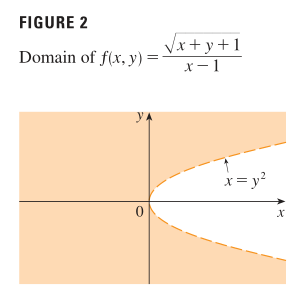
\includegraphics[width = 4.8 cm]{./images/eg1.png} 
  \end{center}
\end{minipage}
\begin{minipage}[]{0.6\linewidth}
{\fontfamily{lmtt}\selectfont \textbf{\textcolor{blue5}{EXAMPLE.}}} 

Evaluate $f(3,2)$,  find and sketch the domain of $f(x,y) = \ln{(y^2 - x)}$.
\[f(3,2) = 3 \ln{(2^2 - 3)} = 3 \ln{1} = 0\]
The domain of $f$ is $D = \{(x, y) \text{ } | \text{ } x < y^2\}$.
\end{minipage}
\subsection*{{\fontfamily{lmss}\selectfont \underline{Graph}}}
\begin{minipage}[]{0.3\linewidth}
  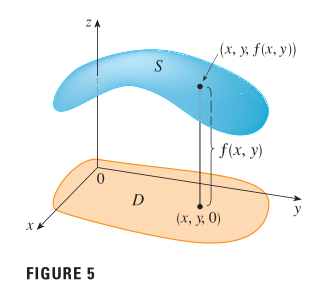
\includegraphics[width = 4 cm]{./images/graph.png}
\end{minipage}
\begin{minipage}[]{0.6\linewidth}
  The graph of $f(x,y)$ is the set of all points $(x,y,z)$ in $\mathbb{R}^3$.
\end{minipage}

{\fontfamily{lmtt}\selectfont \textbf{\textcolor{blue5}{EXAMPLE.}}} Sketch the graph of $f(x,y) = 6 - 3x - 2y$.

\begin{minipage}[]{0.3\linewidth}
  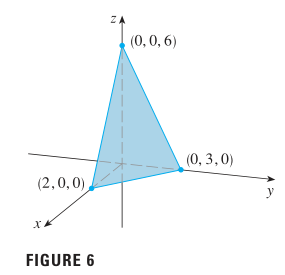
\includegraphics[width = 4 cm]{./images/eg5.png}
  
\end{minipage}
\begin{minipage}[]{0.6\linewidth}
  {\fontfamily{lmtt}\selectfont \textbf{\textcolor{blue5}{A linear function...}}} 

  The equation of the graph is $3x + 2 + z = 6$, which represents a plane. To graph it, find the \textit{intercepts} by setting 2 of the 3 variables to 0.
\end{minipage}

{\fontfamily{lmtt}\selectfont \textbf{\textcolor{blue5}{EXAMPLE.}}} Sketch the graph of $g(x,y) = \sqrt{9 - x^2 - y^2}$.

\begin{minipage}[]{0.34\linewidth}
  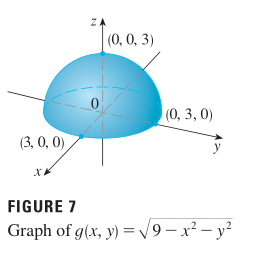
\includegraphics[width = 4 cm]{./images/eg6.png}
  
\end{minipage}
\begin{minipage}[]{0.6\linewidth}
  Square both sides of this equation to obtain $x^2 + y^2 + z^2 = 9$.

  Since $z \ge 0$, this is the upper part of a sphere whose center the origin and radius 3.
\end{minipage}

\pagebreak
Computer programs can graph functions $f(x,y)$. Traces in the vertical planes $x = k$ and $y = k$ are drawn for equally spaced values of $k$ and parts of the graph are eliminated using hidden line removal.
\begin{center}
  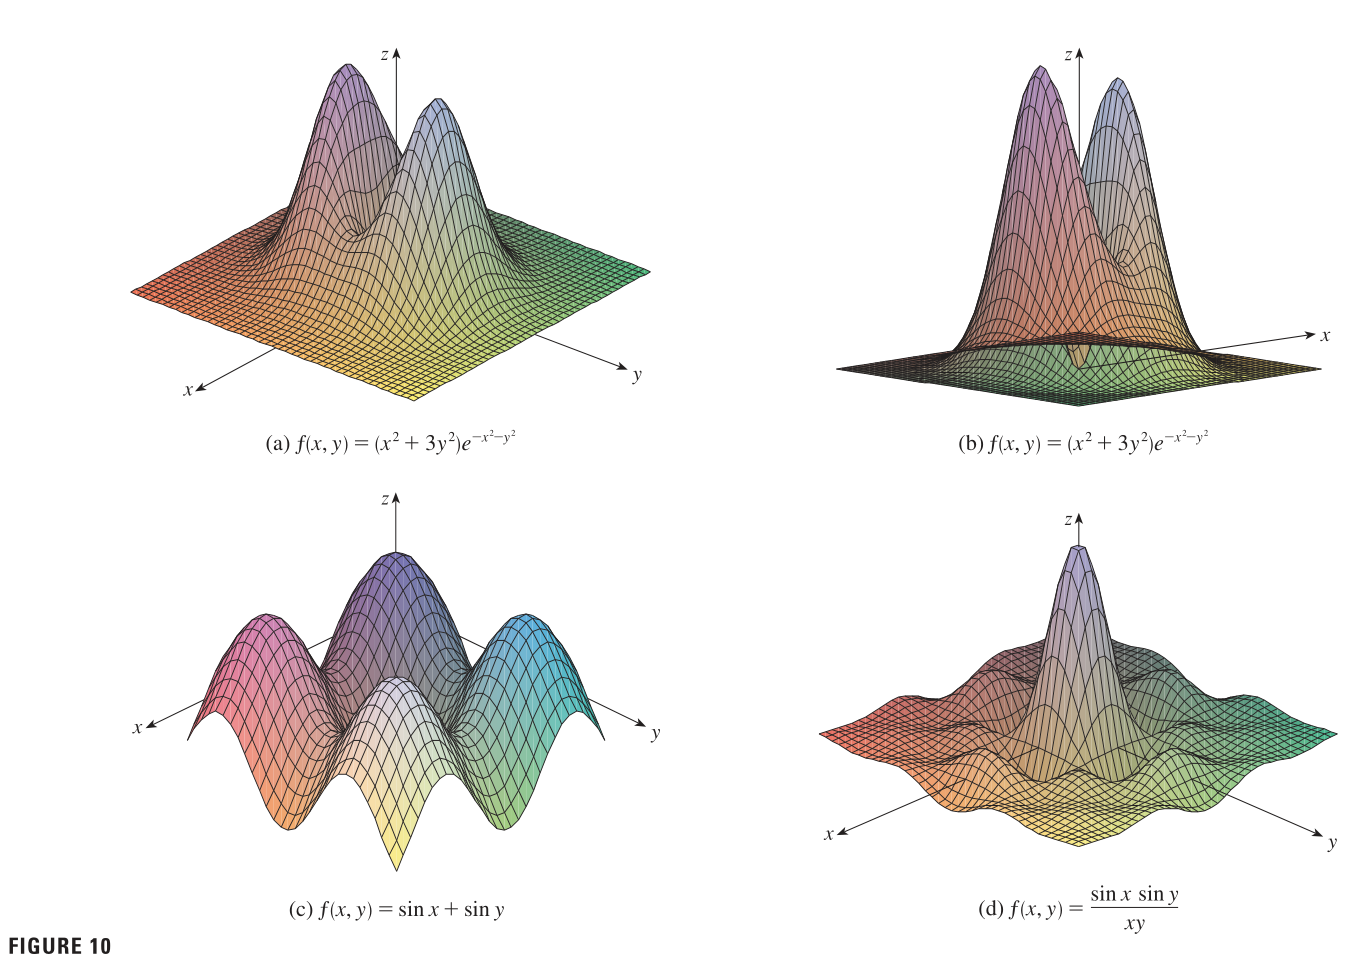
\includegraphics[width = 15 cm]{./images/blender.png} 
\end{center}

\subsection*{{\fontfamily{lmss}\selectfont \underline{Level Curves}}}
Beside arrow diagrams and graphs, we visualize a function using \textit{level curves}, or \textit{contour lines}, formed by a contour map on which points of constant elevation are joined.
\begin{center}
  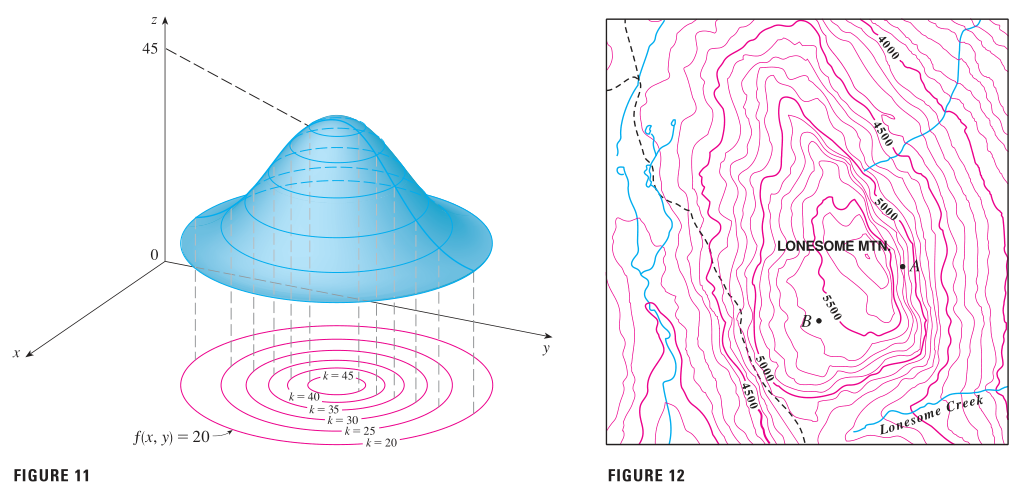
\includegraphics[width = 15 cm]{./images/contour.png} 
\end{center}
Another example of the temperature functions, the level curves are \textbf{isothermals}.
\begin{center}
  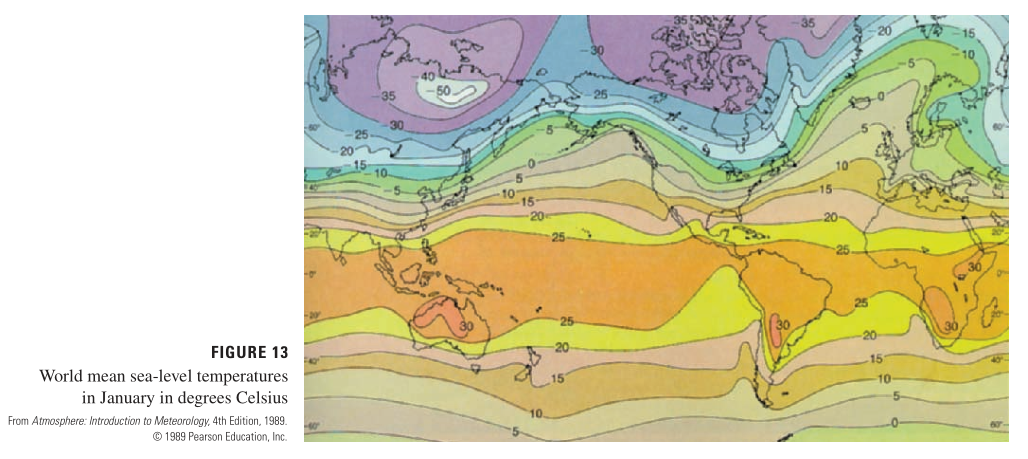
\includegraphics[width = 13.1 cm]{./images/temperature.png} 
\end{center}

For some purpuses, a contour map is more useful than a graph.
\begin{center}
  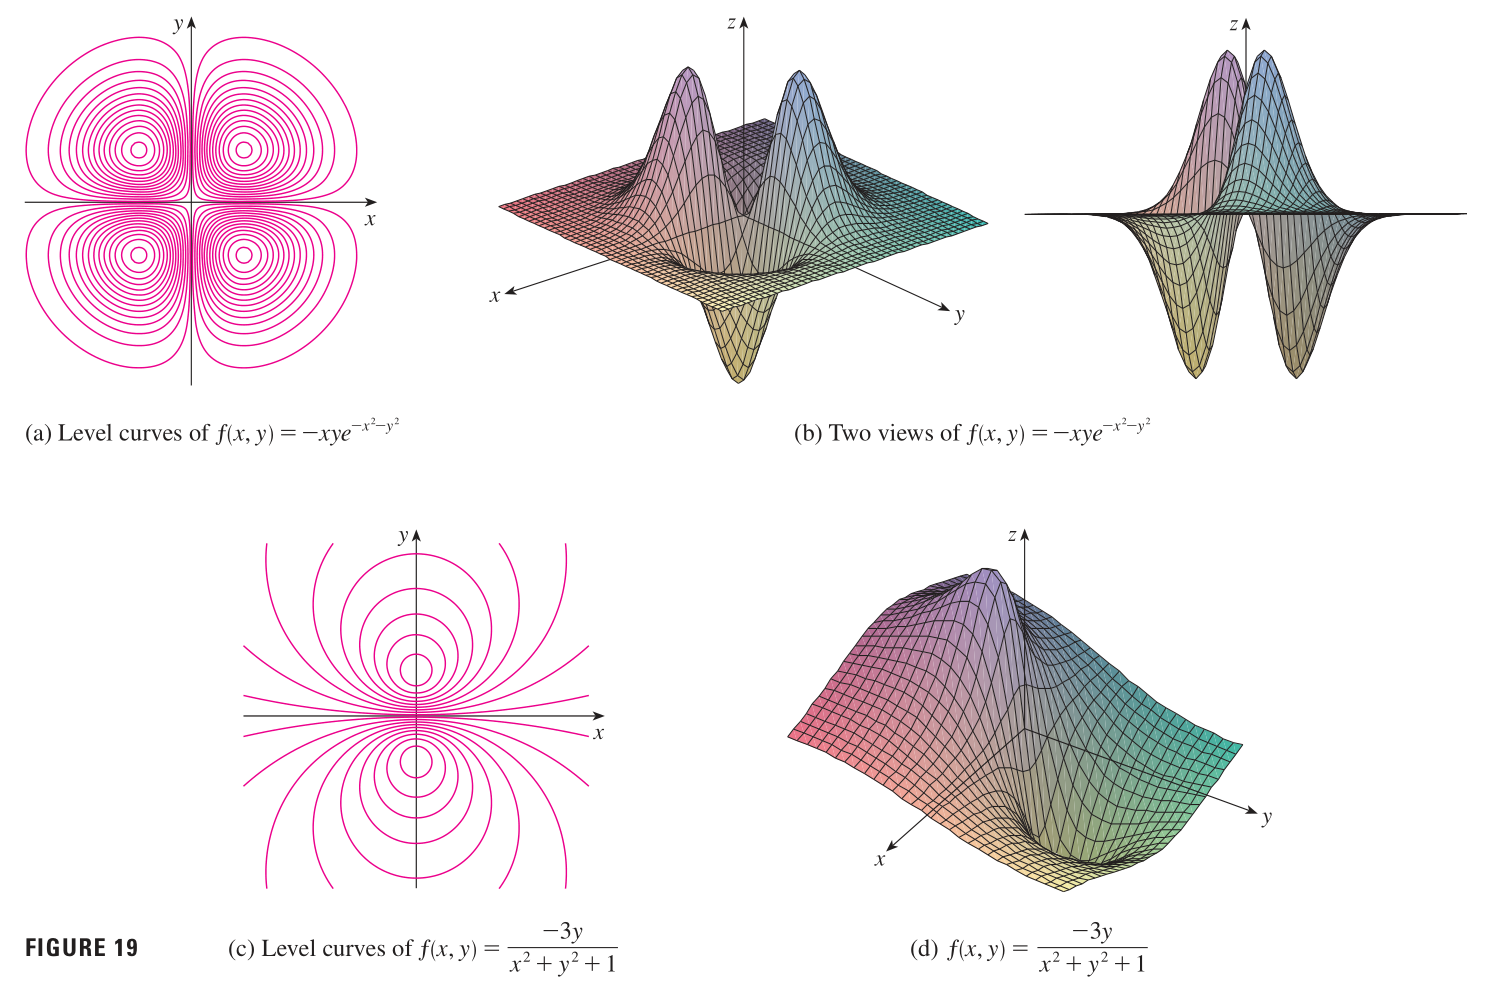
\includegraphics[width = 16 cm]{./images/levelcurves.png} 
\end{center}

\subsection*{{\fontfamily{lmss}\selectfont \underline{Functions of Three or More Variables}}}
It's hard to visualize $f(x,y,z)$ by its graph (four-dimensional space). We examine its \textbf{level surfaces}, which are the surfaces of $f(x,y,z) = k$.

{\fontfamily{lmtt}\selectfont \textbf{\textcolor{blue5}{EXAMPLE.}}} Find the level surfaces of  $f(x,y,z) = x^2 + y^2 + z^2 $.

\begin{minipage}[]{0.35\linewidth}
\begin{center}
  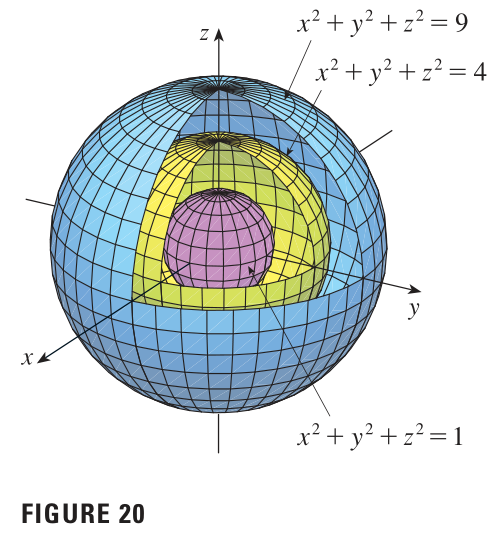
\includegraphics[width = 5 cm]{./images/eg15.png} 
\end{center}
  
\end{minipage}
\begin{minipage}[]{0.6\linewidth}
  The level surfaces are $x^2 + y^2 + z^2 = k \ge 0$, which forms a family of concentric spheres with radius $\sqrt{k}$.
\end{minipage}

\begin{Def}[]
  A \textbf{function of n variables} is a rule that assigns a number $z = f(x_1, x_2 , \cdots , x_n)$ to an $n$-tuple $(x_1, x_2, \cdots, x_n)$. The set of all $n$-tuples is $\mathbb{R}^n$. We can look at it as a function of
  \begin{itemize}
    \item $n$ real variables $x_1, x_2, \cdots, x_n$.
    \item A single point $(x_1, x_2, \cdots, x_n)$.
    \item A single vector $\textbf{x} = \langle x_1, x_2, \cdots, x_n \rangle$
  \end{itemize}
\end{Def}
\pagebreak
\section{Limits and Continuity}
Let's compare 2 functions as $(x,y)$ approach the origin.
\[f(x,y) = \frac{\sin{x^2 + y^2 }}{x^2 + y^2 }   \quad \text{and} \quad g(x,y)= \frac{x^2 - y^2 }{x^2 + y^2 }\]
\begin{center}
  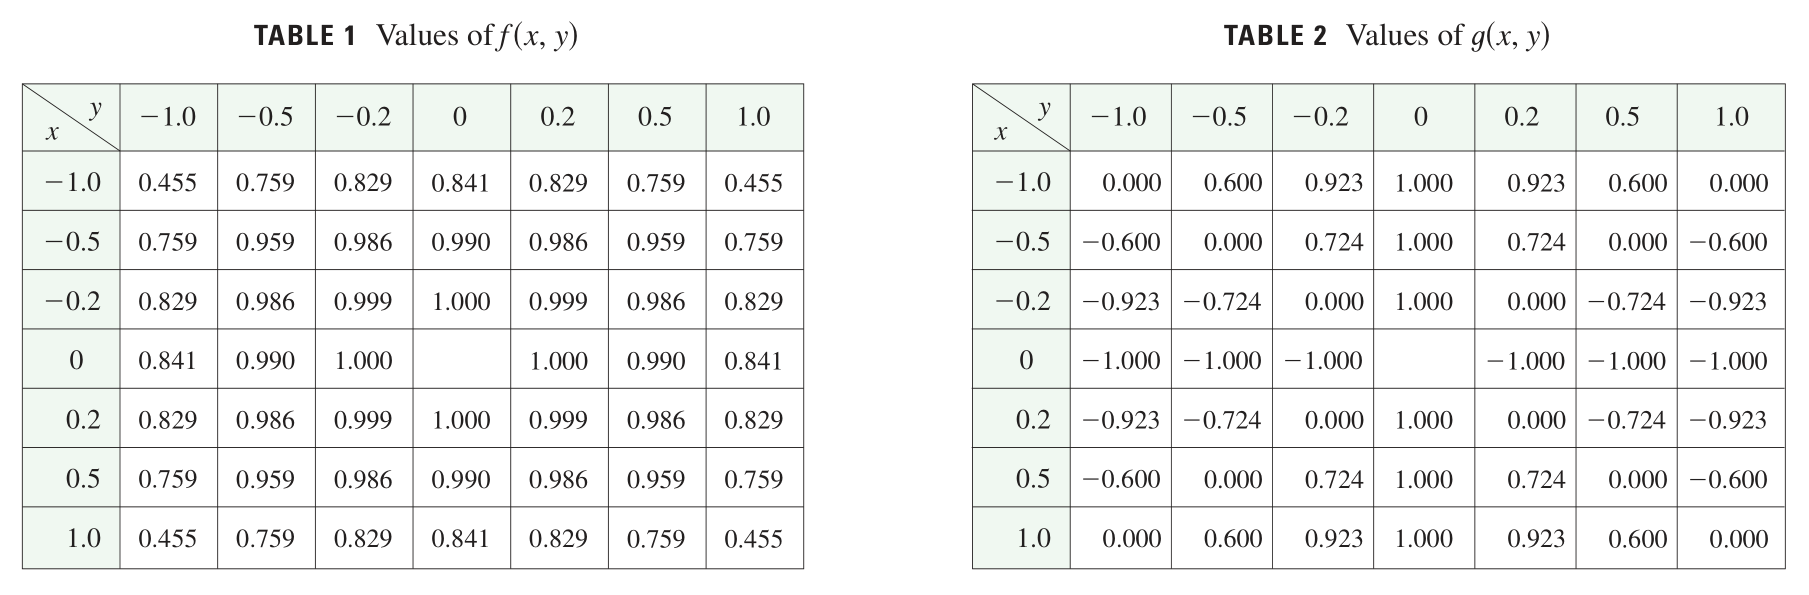
\includegraphics[width = 15 cm]{./images/cmpFG.png}
\end{center}
It appears that $f(x,y)$ are approaching 1 whereas $g(x,y)$ aren't approaching any number.
\begin{Def}[Limit]
The domain $D$ includes points arbitrarily close to $(a,b)$.
 The \textbf{limit of $f(x,y)$ as $(x,y)$ approaches $(a,b)$} is $L$. 
 \[\lim_{(x,y) \to (a,b)} f(x,y) = L\]
 if for $\forall \varepsilon > 0$, there is a corresponding $\delta > 0$ such that 
 \begin{center}
   if $(x,y) \in D$ and $0 < \sqrt{(x - a)^2 + (y - b)^2 } < \delta$ then 
   $f(x,y) - L| < \varepsilon$    
 \end{center}

\end{Def}
   {\fontfamily{lmtt}\selectfont \textbf{\textcolor{blue5}{Note.}}} $|f(x,y) - L|$ is the distance between $f(x,y)$ and $L$. 

   $\quad \sqrt{(x-a)^2 + (y-b)^2}$ is the distance between the  point $(x,y)$ and $(a,b)$ .

  If $(L - \varepsilon, L + \varepsilon     )$ is given, we can find a disk $D_\delta$ with a center $(a,b)$ and radius $\delta > 0$ such that $f$ maps all the points in $D_\delta$ (except possibly $(a,b)$) into $(L - \varepsilon, L + \varepsilon     )$.
  \begin{center}
    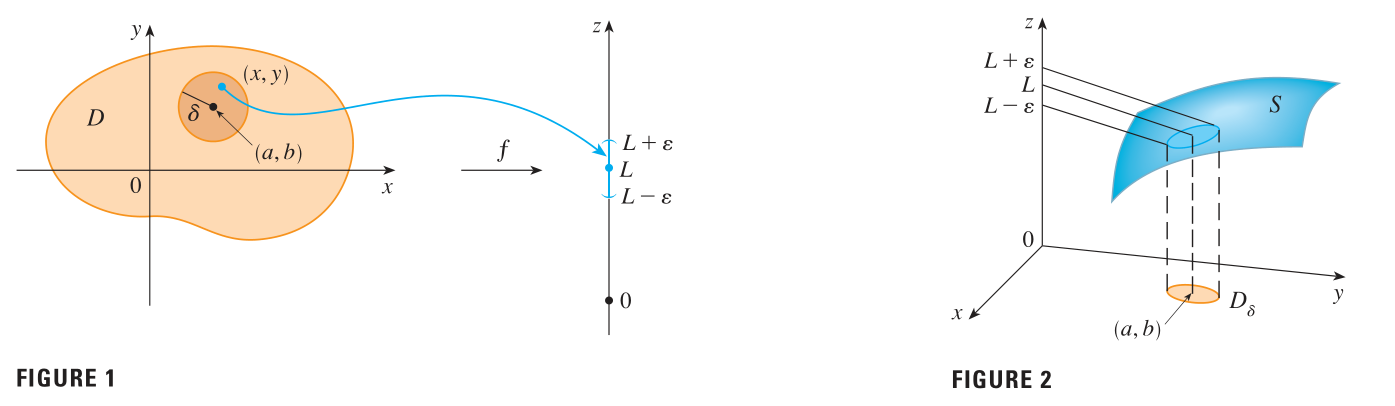
\includegraphics[width = 15 cm]{./images/limit.png} 
  \end{center}
  
  \textbf{1 variable.}   Recall that for $f(x)$, there are only 2 directions of approach, from the left \textit{or} from the right. And if $\lim_{x \to a^{-}} f(x) \ne \lim_{x \to a^{+}} f(x)$, then $lim_{x \to a} f(x)$ does not exist.

  \textbf{2 variables.} We can't just let $(x,y)$ approach $(a,b)$ from an infinite number of directions. But if the limit exists, the $f(x,y)$ must approach the \textbf{same limit} no matter how. 
  \begin{mdframed}
    If $f(x,y) \to L_1$ as $(x,y) \to (a,b)$ along a path $C_1$ and $f(x,y) \to L_2$ as $(x,y) \to (a,b)$ along a path $C_2$, where $L_1 \ne L_2$, then $\lim_{(x,y) \to (a,b)} f(x,y)$ does not exist.
  \end{mdframed}
  {\fontfamily{lmtt}\selectfont \textbf{\textcolor{blue5}{EXAMPLE.}}} Show that  this does not exist \[\lim_{(x,y) \to (0,0)} \frac{x^2 - y^2 }{x^2 + y^2 }\]

  \begin{minipage}[]{0.35\textwidth}
    \begin{center}
      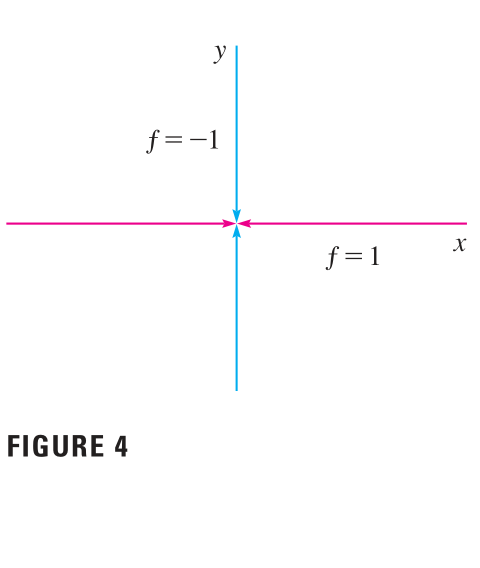
\includegraphics[width = 5 cm]{./images/limeg1.png} 
    \end{center}
  \end{minipage}
  \begin{minipage}[]{0.6\textwidth}
    Let $f(x,y) = (x^2 - y^2 )/(x^2 + y^2 )$. \\ $\square$ First, let approach $(0,0)$ along the $x$-axis.\\
    Then $\quad y = 0$ gives $f(x,0) = x^2 / x^2 = 1$ for $\forall x \ne 0$.
    \begin{center}
    $f(x,y) \to 1  \quad \text{as} \quad (x,y) \to (0,0)$ along the $x$-axis
    \end{center}  
    $\square$ Now, approach along the $y$-axis by putting $x = 0$.\\
    Then $\quad f(0,y) = -y^2 / y^2 = -1$ for $\forall y \ne 0$.
    \begin{center}
      $f(x,y) \to -1 \quad \text{as} \quad (x,y) \to (0,0)$ along the $y$-axis
    \end{center}
    Since $f$ has 2 different limits along 2 different lines, the given limit does not exist.
  \end{minipage}

  {\fontfamily{lmtt}\selectfont \textbf{\textcolor{blue5}{EXAMPLE.}}} Does this limit exist?
  \[\lim_{(x,y) \to (0,0)} f(x,y) = xy/(x^2 + y^2 )\]

    \begin{minipage}[]{0.37\linewidth}
      \begin{center}
        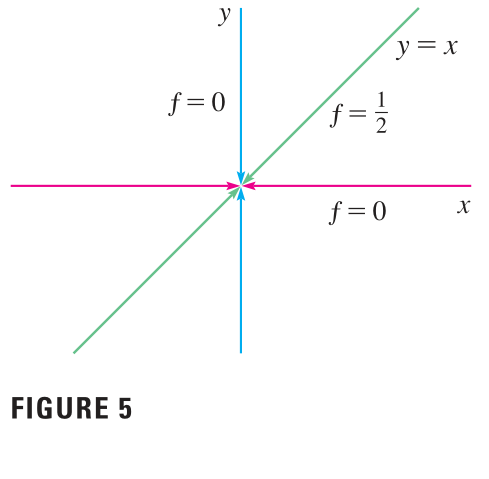
\includegraphics[width = 5 cm]{./images/lim3g2.png} 
      \end{center}
    \end{minipage}
  \begin{minipage}[]{0.6\linewidth}
    $\square$ If $y = 0$, then $f(x,0) = 0/ x^2 $
    \begin{center}
      $f(x,y) \to 0 \quad \text{as} \quad (x,y) \to (0,0)$ along the $x$-axis
    \end{center}
    $\square$ If $x = 0$, then $f(0,y) = -/ y^2 = 0$, so 
    \begin{center}
      $f(x,y) \to 0 \quad \text{as} \quad (x,y) \to (0,0)$ along the $y$-axis
    \end{center}
  \end{minipage}
Although we have obtained identical limits along the axes, that does not show the answer is 0.  \\
$\square$ Let's approach $(0,0)$ along another line, say $y = x$. For all $x \ne 0$,
\[f(x,x) = \frac{x^2 }{x^2 + x^2 } = \frac{1}{2}\]
Therefore $\quad f(x,y) \to \frac{1 }{2 } \quad \text{as} \quad (x,y) \to (0,0)$  along $y = x$. The given limit \textbf{does not exist}. 

The ridge that occurs above the line $y = x$ correspond to the fact that $f(x,y) = \frac{1 }{2 }$ for all points $(x,y)$ on that line \textbf{except the origin}.
\begin{center}
  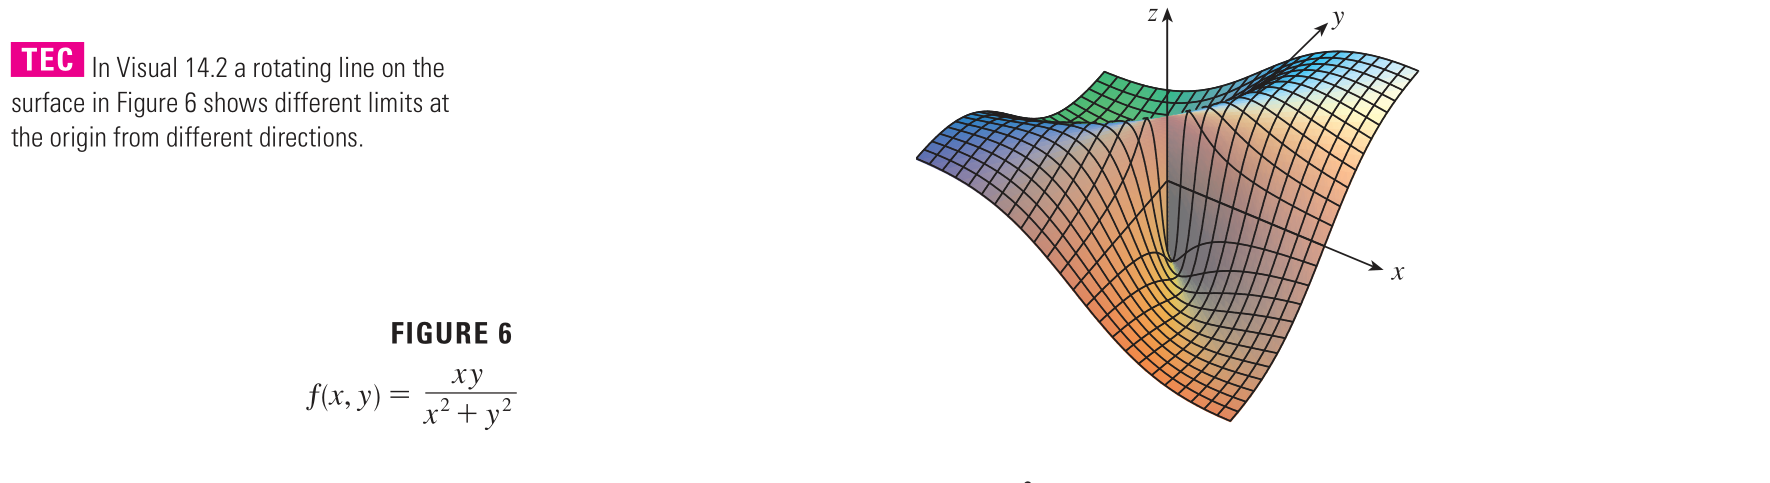
\includegraphics[width = \linewidth]{./images/limeg2.png} 
\end{center}
{\fontfamily{lmtt}\selectfont \textbf{\textcolor{blue5}{EXAMPLE.}}} Find the limit.
\[\lim_{(x,y) \to (0,0)} \frac{x y^2 }{x^2 + y^4}\]
Let's approach along any nonvertical line through the origin. Then $y = mx$, where $m$ is the slope, then
\[f(x,y) = f(x, mx) = \frac{x(mx)^2}{x^2 + (mx)^4} = \frac{m^2 x^3}{x^2 + m^4 x^4} = \frac{m^2 x}{1 + m^4 x^2}\]
So $\quad f(x,y) \to 0 \quad \text{as} \quad (x,y) \to (0,0)$ along $y = mx$.\\
Thus $f$ has the same limiting value along \textit{every nonvertical line} through the origin. But that does not show that the answer is 0, if we now let $(x,y) \to (0,0)$ along the parabola $x = y^2$, we have 
\[f(x,y) = f(y^2, y) = \frac{y^2 \cdot y^2 }{(y^2 )^2 + y^4} = \frac{y^4}{2y^4} = \frac{1 }{2 }\]
Hence, the limit \textbf{does not exist}.

\begin{mdframed}
 \textbf{What limits that do exist then?} 

 The limit of a \textbf{sum} the sum of the limits, so does a \textbf{product}. These equations are true.
 \begin{align*}
   \lim_{(x,y) \to (a,b)} x = a & \quad & \lim_{(x,y) \to (a,b)} y = b & \quad & \lim_{(x,y) \to (a,b)} c = c 
 \end{align*}
 The Squeeze Theorem also holds.
\end{mdframed}
{\fontfamily{lmtt}\selectfont \textbf{\textcolor{blue5}{EXAMPLE.}}} Find the limit.
\[\lim_{(x,y) \to (0,0)}\frac{3 x^2 y }{x^2 + y^2 }\]
$\square$ As the previous example, we see that the limit along any line through the origin is 0. Plus, the limits along the parabolas $y = x^2$ and $x = y^2$ are also 0, so we suspect the limit exist and equal to 0.\\
$\square$ Let $\varepsilon > 0$. We want to find $\delta > 0 $ such that 
\[\text{if } \quad 0 < \sqrt{x^2 + y^2 } < \delta \quad \text{ then } \quad \abs{ \frac{3x^2 y }{x^2 + y^2 } - 0  } < \varepsilon \]
That is, 
\[\text{if } \quad 0 < \sqrt{x^2 + y^2 } < \delta \quad   \text{ then } \quad  \frac{3x^2 |y| }{x^2 + y^2   } < \varepsilon \]
Since $ x^2 \le x^2 + y^2 $, so $x^2 / (x^2 + y^2 ) \le 1$ and therefore 
\[\frac{3 x^2 |y| }{x^2 + y^2 } \le 3 |y| = 3 \sqrt{y^2 } \le 3 \sqrt{x^2 + y^2 } < 3 \delta \]
Thus we choose $\delta = \varepsilon / 3 $ and let $0 < \sqrt{x^2 + y^2 } < \delta $, then 
\[\frac{3 x^2 |y| }{x^2 + y^2 } \le 3 \sqrt{x^2 + y^2 } < 3 \delta = 3 \left(\frac{\varepsilon }{3 }\right) = \varepsilon   \]
Hence, by the \textbf{Definition: Limit}, 
\[\lim_{(x,y) \to (0,0)} \frac{3 x^2 y }{x^2 + y^2 } = 0 \]

\subsection*{{\fontfamily{lmss}\selectfont \underline{Continuity}}}
Limits of \textit{continuous} functions is easy evaluated by direct substitution.
\begin{Def}[Continuity]
  A function $f$ is \textbf{continuous at $(a,b)$} if 
  \[\lim_{(x,y) \to (a,b)} f(x,y) = f(a,b)\]
  We say $f$ is \textbf{continuous on $D$} if $f$ is continuous at \textit{every} point $(a,b)$ in $D$.
\end{Def}
A \textbf{polynomial function of 2 variables} is a sum of terms $c x^m y^n$, and a \textbf{rational function} is a ratio of polynomials. For instance,
\[f(x,y) = x^4 + 5x^3 y^2 + 6xy^4 - 7y + 6  \]
is a polynomial, whereas 
\[g(x,y) = \frac{2xy + 1 }{x^2 + y^2 }\]
is a  rational function. A rational function is $continuous$ on its domain because it's a quotient of continuous functions (polynomial).\\
{\fontfamily{lmtt}\selectfont \textbf{\textcolor{blue5}{EXAMPLE.}}} 
\[ \lim_{(x,y) \to (1,2)} (x^2 y^3 - x^3 y^2 + 3x + 2y) = 1^2 \cdot 2^3  - 1^3 \cdot 2^2 + 3 \cdot 1 + 2 \cdot 2 = 11 \]
{\fontfamily{lmtt}\selectfont \textbf{\textcolor{blue5}{EXAMPLE.}}} Let 
\[ g(x,y) = 
\begin{cases}
  \frac{x^2 -y^2 }{x^2 + y^2 } \quad \text{if} \quad (x,y) \ne (0,0) \\
  0 \quad \quad \text{ if } \quad (x,y) = (0,0)
\end{cases}\]
Here $g$ is defined at $(0,0)$ but still discontinuous because $\lim_{(x,y) \to  (0,0)} g(x,y)$ does not exist.
\pagebreak 
\begin{mdframed}
{\fontfamily{lmtt}\selectfont \textbf{\textcolor{blue5}{Composition.}}} If $f(x,y)$ is continuous, and so is $g(x)$, then the composite function $h = g \circ f$, defined by $h(x,y) = g(f(x,y))$ is continuous.
  
\end{mdframed}

\begin{minipage}[]{0.34\linewidth}
  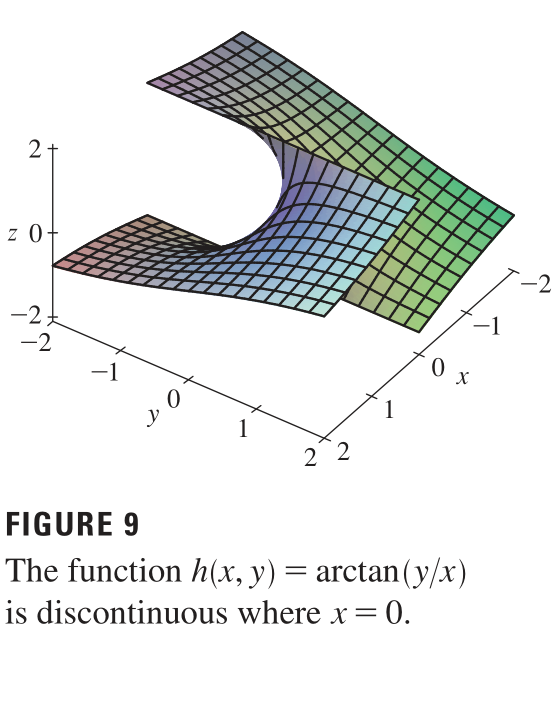
\includegraphics[width = 4.6 cm]{./images/arctanyx.png}
  
\end{minipage}
\begin{minipage}[]{0.57\linewidth}
{\fontfamily{lmtt}\selectfont \textbf{\textcolor{blue5}{EXAMPLE.}}} Where is the function $h(x,y) = \arctan(y/x)$ continuous?

The function $f(x,y) = y/x$ is a rational function, and therefore continuous except on the line $x = 0$. The function $g(t) = \arctan{t}$ is continuous everywhere. So the composite function $g(f(x,y))$ is continuous except where $x = 0$.
  
\end{minipage}

\subsection*{{\fontfamily{lmss}\selectfont \underline{Functions of Three or More Variables}}}
It's just the same. For every number $\varepsilon > 0$, there is a corresponding number $\delta > 0$ such that 
\begin{center}
  if $\quad (x,y,z) $ is in the domain of $f\quad $ and $\quad 0 < \sqrt{(x- a)^2 + (y - b)^2 + (z-c)^2 } < \delta $ \\
  then $\quad \abs{f(x,y,z) - L} < \varepsilon $
\end{center}

The function $f$ is \textbf{continuous} at $(a,b,c)$ if 
\[\lim_{(x,y,z) \to (a,b,c)} f(x,y,z) = f(a,b,c )\]
{\fontfamily{lmtt}\selectfont \textbf{\textcolor{blue5}{EXAMPLE.}}} The function \[f(x,y,z) = \frac{1 }{x^2 + y^2 + z^2 - 1 }\] is a rational function, so it's continuous at every point of $\mathbb{R}^3$ except where $x^2 + y^2 + z^2 = 1 $.  In other words, it's discontinuous on the sphere with center the origin and radius 1.

\begin{Def}[Limit in $\mathbb{R}^n$]
  If $\lim_{x \to a } f (\textbf{x}) = L$, then it means that for every number $\varepsilon > 0 $ there is a corresponding $\delta > 0$ such that 
  \[\text{if } \quad x \in D \quad \text{and } \quad 0 < \abs{\textbf{x} - \textbf{a}} < \delta \quad \text{then } \quad \abs{f(\textbf{x}) - L} < \varepsilon \]
\end{Def}


\section{Partial Derivatives}
Suppose we let $x$ vary while keeping $y$ fixed ($y = b$) in $f(x,y)$, we got a function $g(x) = f(x,b)$. If $g$ has a derivative at $a$, we call it the \textbf{partial derivative of \textit{f} with respect to \textit{x} at \textit{(a,b)}}. We have 
\[g'(a) = \lim_{h \to  0 }\frac{g(a + h) - g(a)}{h }\]
and so it become $\quad$
\begin{minipage}[]{0.6\linewidth}
\begin{mdframed}
\[f_x (x,y) = \lim_{h \to 0} \frac{f(x + h, b) - f(x,y)}{h }\]
\[f_y (x,y) = \lim_{h \to 0} \frac{f(x , y + h) - f(x,y)}{h }\]
  \end{mdframed}
\end{minipage}

To compute partial derivatives, we have the following rule.
\begin{mdframed}
  {\fontfamily{lmtt}\selectfont \textbf{\textcolor{blue5}{\small $\blacksquare$ Rule for Finding Partial Derivatives of $z = f(x,y)$}}} \\
{\fontfamily{lmtt}\selectfont \textbf{\small 1.}} To find $f_x$, regard $y$ as a constant and differentiate $f(x,y)$ with respect to $x$.\\
{\fontfamily{lmtt}\selectfont \textbf{\small 2.}} To find $f_y$, regard $x$ as a constant and differentiate $f(x,y)$ with respect to $y$.
\end{mdframed}
{\fontfamily{lmtt}\selectfont \textbf{\textcolor{blue5}{{\small \faIcon{map-marker-alt}} EXAMPLE.}}} If $f(x,y) = x^3 + x^2 y^3 - 2y^2$, find $f_x(2,1)$ and $f_y(2,1)$.
Holding $y$ constant and differentiating with respect to $x$, we get 
\begin{equation*}
  \begin{split}
 &   f_x(x,y) = 3 x^2 + 2x y^3 \\
 &  f_x(2,1) = 3 \cdot 2^2 + 2 \cdot 2 \cdot 1^3 = 16
  \end{split}
\end{equation*}
Do the same with $y$
\begin{equation*}
  \begin{split}
    & f_y (x,y) = 3 x^2 y^2 - 4y \\
    & f_y (2,1) = 3 \cdot 2^2 \cdot 1^2 - 4 \cdot 1 = 8       
  \end{split}
\end{equation*}

\subsection*{{\fontfamily{lmss}\selectfont \underline{Interpretations of Partial Derivatives}}}

\begin{minipage}[]{0.34\linewidth}
  \begin{center}
    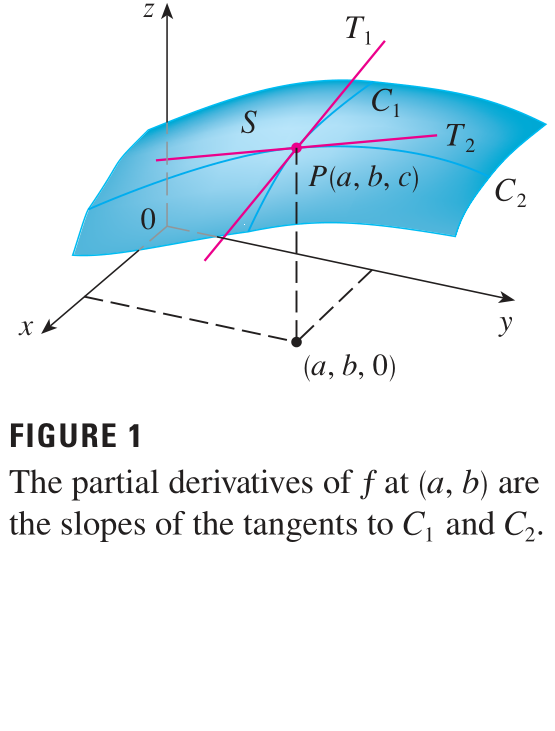
\includegraphics[width = 4.3 cm]{./images/interpretation.png} 
  \end{center}
\end{minipage}
\begin{minipage}[]{0.6\linewidth}
\textcolor{blue5}{\small $\blacksquare$}  The equation $f(x,y)$ represent a surface $S$. By fixing $y = b$, we got the curve $C_1$ (the trace of $S$ in the pane $y = b $).

\textcolor{blue5}{\small $\blacksquare$}  Notice that $C_1 $ is the graph of $g(x) = f(x, b )$, so the slope of its tangent $T_1$ is $g'(a) = f_x(a,b)$.
\end{minipage}

\begin{minipage}[]{0.34\linewidth}
  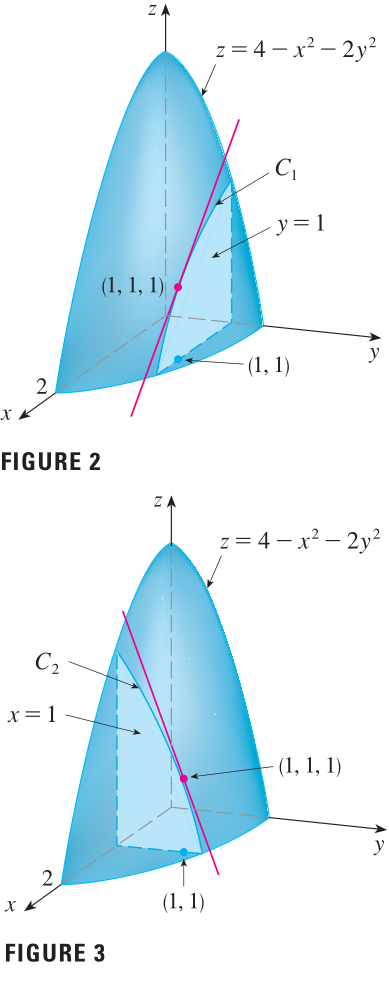
\includegraphics[width = 4  cm]{./images/pareg2.png}
  
\end{minipage}
\begin{minipage}[b]{0.63\linewidth}

 {\fontfamily{lmtt}\selectfont \textbf{\textcolor{blue5}{{\small \faIcon{map-marker-alt}} EXAMPLE.}}} If $f(x,y) = x^3 + x^2 y^3 - 2 y^2 $, find $f_x (1,1)$ and $f_y (1,1)$ and interpret these numbers as slopes.

 We have 
 \begin{equation*}
   \begin{split}
      f_x (x,y) = -2x & \quad \text{ } \quad f_y (x.y) = -4y \\
      f_x(1,1) = -2 & \quad  \text{ } \quad f_y(1,1) = -4  
   \end{split}
 \end{equation*}
 
 The vertical plane $y = 1 $ intersects $f(x,y)$ in the parabola $z = 2 - x^2 $, $y = 1$ ($C_1$). The slope of the tangent line to this parabola at the point $(1,1,1)$ is $f_x (1,1) = -2 $.
\end{minipage}\\
{\fontfamily{lmtt}\selectfont \textbf{\textcolor{blue5}{{\small \faIcon{map-marker-alt}} EXAMPLE.}}} If $f(x,y) = \sin{\left(\cfrac{x }{1 + y }\right)}$, calculate $\cfrac{\delta f }{\partial x }$ and $\cfrac{\delta f}{\partial y}$.

\textcolor{blue5}{\small $ \blacksquare$} Using the Chain Rule for functions of one variable, we have 
\begin{equation*}
  \begin{split}
    & \frac{\partial f }{\partial x } = \cos{\left( \frac{x }{ 1 + y }  \right)} \cdot \frac{\partial}{\partial x } \left( \frac{x }{1 + y }  \right) = \cos{ \left( \frac{x }{1 + y }\right)} \cdot \frac{1 }{1 + y } \\ 
    & \frac{\delta f }{\partial y } = \cos{\left( \frac{x }{ 1 + y }  \right)} \cdot \frac{\partial }{\partial y } \left( \frac{x }{1 + y }  \right) = -  \cos{ \left( \frac{x }{1 + y }\right)} \cdot \frac{x }{(1 + y)^2 } 
  \end{split}
\end{equation*}
{\fontfamily{lmtt}\selectfont \textbf{\textcolor{blue5}{{\small \faIcon{map-marker-alt}} EXAMPLE.}}} Find $\partial z / \partial x $ and $ \partial z / \partial y $ of $z $ is defined as follow 
\[x ^ 3 + y ^ 3 + z ^ 3 + 6 xyz = 1 \]


\begin{minipage}[b]{0.28\linewidth}
  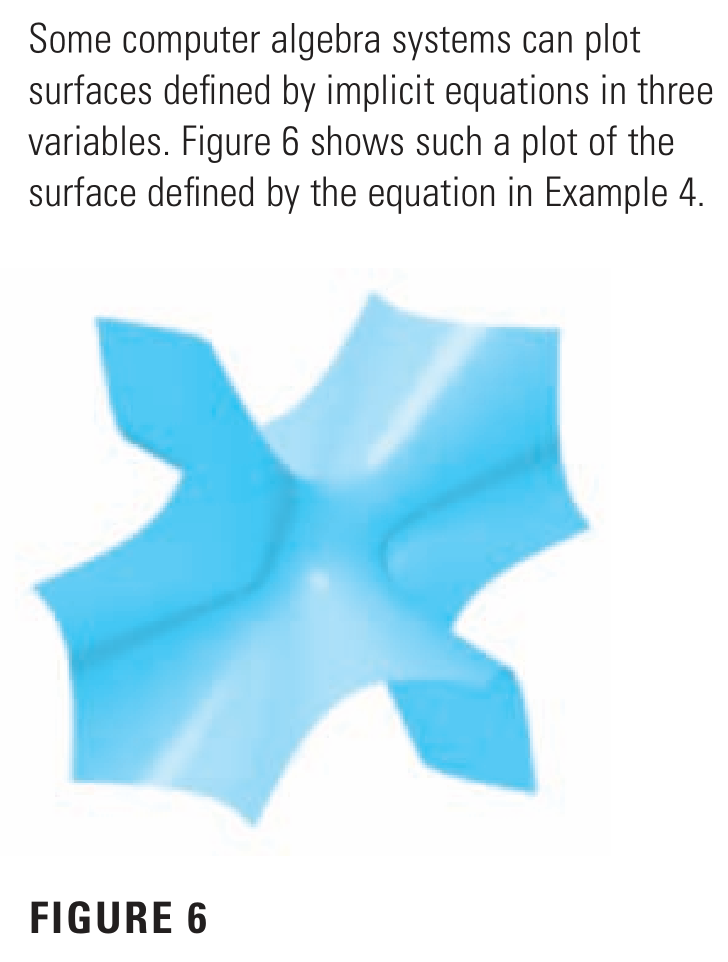
\includegraphics[width = 4.3 cm]{./images/partialeg4.png}
  \end{minipage}
\begin{minipage}[b]{0.67\linewidth}
\textcolor{blue9}{\small $\blacksquare$} First differentiate implicitly with respect to $x $, treat $y $ as a constant.
\[3 x^2 + 3 z^2 \frac{\partial z }{ \partial x } + 6yz + 6xy \frac{\partial z }{ \partial x }= 0\]
Solving this for $\partial z / \partial x $, we obtain 
\[ \frac{\partial z }{\partial x } = - \frac{y^2 + 2xz }{z^2 + 2xy }\]
Similarly, implicit differentiation with respect to $y $ gives 
\[\frac{\partial z }{\partial y } = - \frac{y^2 + 2xz }{z^2 + 2xy }\]
\end{minipage}

\subsection*{{\fontfamily{lmss}\selectfont \underline{Functions of More Than Two Variables }}}  
Regarding $y$ and $z$ as constants and differentiating with respect to $x$.
\[f_x (x, y, z) = \lim_{h \to 0 } \frac{f(x + h, y, z) - f(x,y,z)}{h }\]
{\fontfamily{lmtt}\selectfont \textbf{\textcolor{blue5}{{\small \faIcon{map-marker-alt}} EXAMPLE.}}}  Find $f_x, f _ y $, and $f _ z $ if $f(x,y,z) = e^{xy} \ln{z}$.

Holding $y$ and $z $ constant and differentiating with respect to $x $, we have 
\[f_x = y e^{xy} \ln{z}\]

Similarly, \[f_y = x e^{xy} \ln {z} \quad  \text{and} \quad f_z = \cfrac{e^{xy}}{z }\]

\subsection*{{\fontfamily{lmss}\selectfont \underline{Higher Derivatives}}}

If $f$ is a function of 2 variables, then $f_x$ and $f _ y $ are also functions of 2 variables.  So we can consider the \textbf{second partial derivatives} of $f$, that is $(f_x)_x$, $(f_x)_y $, $(f_y)_x $, and $(f_y)_y $.
\begin{equation*}
  \begin{split}
    & (f _ x ) _ x = f _ {xx} = f _ {11} = \frac{\partial }{\partial x } \left( \frac{\partial f }{ \partial x }\right) = \frac{\partial ^2 f }{\partial  x^2 } = \frac{\partial ^2 z }{\partial x^2 } \\
    & (f _ x ) _ y = f _ {xy} = f _ {12} = \frac{\partial }{\partial y } \left( \frac{\partial f }{ \partial x }\right) = \frac{\partial ^2 f }{\partial  y \text{ } \partial x } = \frac{\partial ^2 z }{\partial y \text{ }\partial x } \\
    & (f _ y ) _ x = f _ {yx} = f _ {21} = \frac{\partial }{\partial x } \left( \frac{\partial f }{ \partial y }\right) = \frac{\partial ^2 f }{\partial  x \text{ } \partial y } = \frac{\partial ^2 z }{\partial x \text{ }\partial y } \\
& (f _ y ) _ y = f _ {yy} = f _ {22} = \frac{\partial }{\partial y } \left( \frac{\partial f }{ \partial y }\right) = \frac{\partial ^2 f }{\partial  y^2 } = \frac{\partial ^2 z }{\partial y^2 }
  \end{split}
\end{equation*}
Thus $f_{xy}$ (or $\partial ^2 f / \partial y \text{ } \partial x $) means that we first differentiate with respect to $x $ and then with respect to $y $.\\
{\fontfamily{lmtt}\selectfont \textbf{\textcolor{blue5}{{\small \faIcon{map-marker-alt}} EXAMPLE.}}} Find the second partial derivatives of 
\[f(x,y) = x ^ 3 + x^2 y^3 - 2 y^2 \]
{\fontfamily{lmss}\selectfont \textcolor{blue5}{\small SOLUTION}} We find that 
\[f_x(x,y) = 3 x^2 + 2x y^3 \quad \text{ } \quad f_y(x,y) = 3 x^2 y^2 - 4y \]
Therefore 
\begin{equation*}
  \begin{split}
    f _ {xx} = \frac{\partial }{\partial x } (3 x^2 + 2xy^3)  = 6x + 2 y^3 & \quad \text{ }  \quad f _ {xy} = \frac{\partial }{ \partial y } (3 x^2 + 2 x y^3) = 6x y^2 \\
    f _ {yx} = \frac{\partial }{\partial x } (3 x^2 y^2 - 4y) = 6x y^2 & \quad \text{ } \quad f_{yy} = \frac{\partial }{\partial y } (3 x^2 y^2 - 4y ) = 6 x^2 y - 4 
  \end{split}
\end{equation*}
\begin{mdframed}
  \textbf{\textcolor{pink}{\fontfamily{lmss}\selectfont Clairaut's Theorem}} $\quad$ Suppose $f $ is defined on a disk $D $ that contains the point $(a, b )$. If the functions $f _ {xy}$ and $f _ {yx }$ are both continuous in $D $, then 
  \[f _ {xy} (a, b) = f _ {yx} (a, b )\]
\end{mdframed}
Partial derivatives of order 3 or higher can also be defined
\[f _ {xyy} = (f _ {xy}) _ y = \frac{\partial }{ \partial y } \left( \frac{\partial ^2 f }{\partial x \text{ } \partial y }\right) = \frac{\partial ^3 f }{\partial y^2 \text{ } \partial x}\]
and using Clairaut's Theorem it can be shown that $f _ {xyy} = f _ {y xy} = f _ {yy x }$. \\
{\fontfamily{lmtt}\selectfont \textbf{\textcolor{blue5}{{\small \faIcon{map-marker-alt}} EXAMPLE.}}} Calculate $f _ {xxyz}$ if $f(x,y,z) = \sin{3x + yz}$. \\
\textbf{\textcolor{blue5}{\fontfamily{lmss}\selectfont \small SOLUTION.}} $\quad $ 
\begin{equation*}
  \begin{split}
     f _ {x} & = 3 \cos{(3x + yz) } \\
     f _ {xx} & = -9 \sin{(3x + yz)} \\
     f _ {xxy} & = -9z \cos{(3x + yz)} \\
     f _ {xxyz} & = -9 \cos{(3x + yz)} + 9yz \sin{(3x + yz)}
  \end{split}
\end{equation*}

\subsection*{{\fontfamily{lmss}\selectfont \underline{Partial Differential Equations}}}
\textbf{Laplace's equation.}
$$\cfrac{\partial ^2 u }{\partial x^2 } + \cfrac{\partial ^2 u }{\partial y^2 } = 0 $$

\section{Tangent Planes and Linear Approximations}
As we zoom in toward a point on a surface of a differentiable function, the surface looks more and more like a plane (its tangent plane) and we can approximate it by a linear function of 2 variables.

\begin{minipage}[b]{0.34\linewidth}
  \begin{center}
    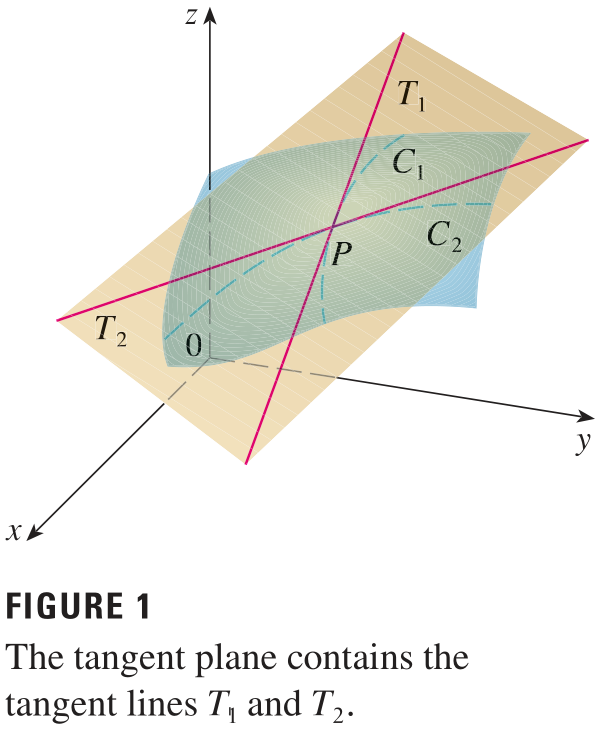
\includegraphics[width = 4.3 cm]{./images/tangentplane.png} 
  \end{center}
  
\end{minipage}
\begin{minipage}[b]{0.63\linewidth}
  \subsection*{{\fontfamily{lmss}\selectfont \underline{Tangent Planes}}}
  Suppose surface $S$ of $z = f(x,y)$ has continuous first partial derivatives, let $P(x _ 0,  y _ 0, z _ 0 ) \in S$. \\
  \textcolor{blue5}{$\blacksquare$} $C _ 1 $ and $C _ 2 $ be the curves obtained by intersecting the vertical planes $y = y _ 0 $ and $ x = x0 $ with $S $.\\
 \textcolor{blue5}{$\blacksquare$} Let $T _ 1 $  and $T _ 2 $ be the tangent lines to the curves  $C _ 1 $ and $ C _ 2$ at $P$. 
 Then the \textbf{tangent plane} to the surface $S $ at the point $P $ contains $T _ 1 $ and $T _ 2 $. In fact, it consists of \textit{all possible} tangent lines at $P $.\\
\textcolor{blue5}{$\blacksquare$} We know the plane has an equation of the form 
\[A(x - x _ 0) + B(y - y _ 0) + C(z - z _ 0 ) = 0 \]
By dividing this by $C $ and letting $a = -A/C $ and $b = -B/C $, 
\[z - z _ 0 =  a(x - x _ 0 ) + b (y - y _ 0 )\]
\end{minipage}

The tangent plane's intersection with the plane $y = y _ 0 $ must be the tangent line $T _ 1 $.
\[z - z _ 0 = a(x - x _ 0 ) \quad \text{ where } y = y _ 0\]

This is a line with slope $a = f _ x (x _ 0, y _ 0  )$. Similarly, $z - z _ 0 = b ( y - y _ 0 )$, and $b = f _ y (x _ 0, y _ 0 )$.

\begin{Def}[Equation of Tangent Plane]
  Suppose $f $ has continuous partial derivatives. An equation of the tangent plane to the surface $z = f(x,y) $ at the point $P(x _ 0, y _ 0, z  _ 0 )$ is 
  \[z - z _ 0 = f_x(x _ 0, y _ 0) (x - x _ 0) + f_y (x _ 0, y _ 0) (y - y _ 0 )\]
\end{Def}
{\fontfamily{lmtt}\selectfont \textbf{\textcolor{blue5}{{\small \faIcon{map-marker-alt}} EXAMPLE.}}} Find the tangent plane to the elliptic paraboloid $z = 2 x^2  + y^2 $ at the point (1, 1, 3).
\begin{align*}
  &f_x(x,y) = 4x & & f_y(x,y) = 2y \\ 
  &f_x(1,1) = 4 & & f_y(1,1) = 2 
\end{align*}    
Then the equation of the tangent plane at (1, 1, 3) is 
\begin{equation*}
  \begin{split}
    z - 3 & = 4(x-1) + 2(y - 1) \\
    z & = 4x + 2y - 3 
  \end{split}
\end{equation*}
\begin{center}
  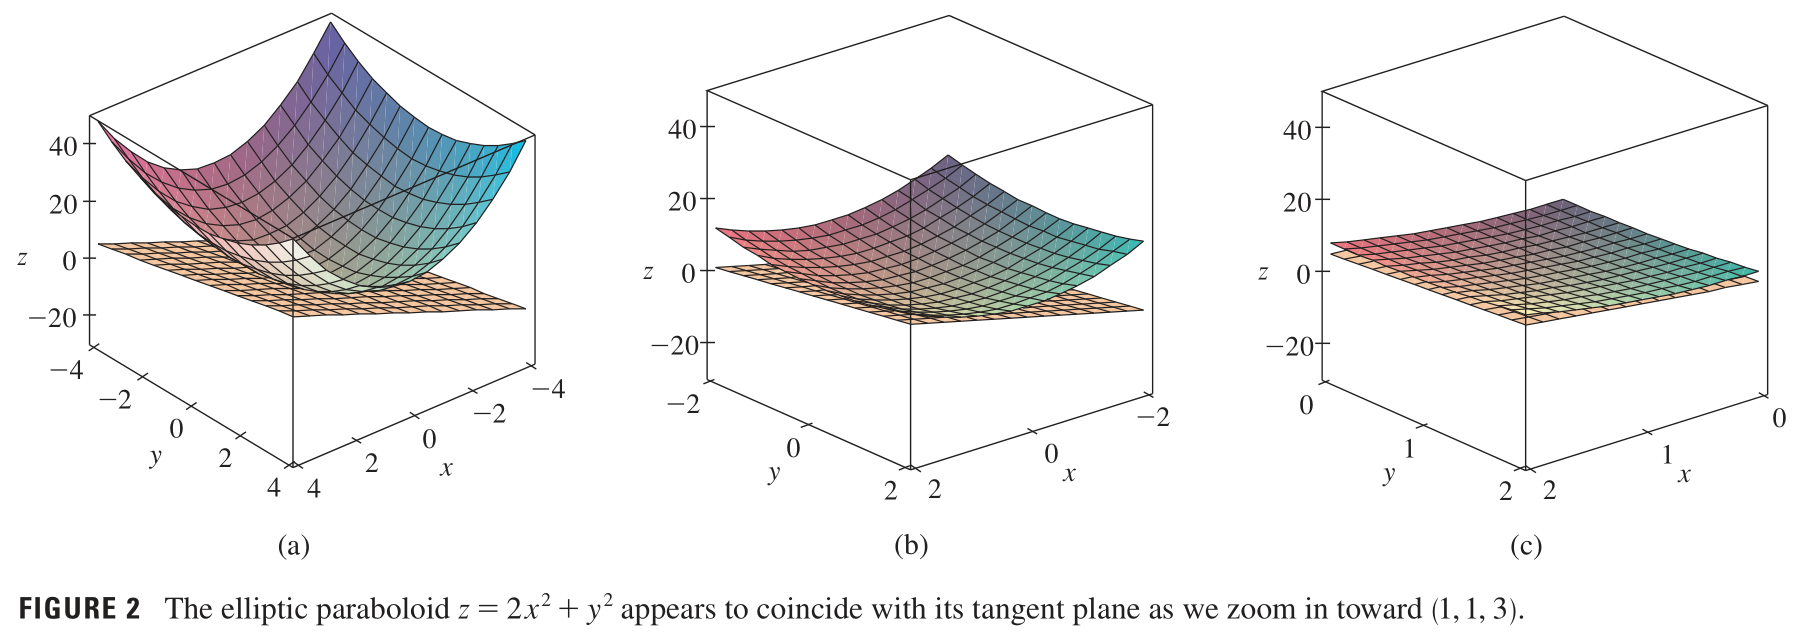
\includegraphics[width = 16 cm]{./images/tangent1.png} 
\end{center}

\begin{minipage}[]{0.34\linewidth}
\hfill  
\end{minipage}
\begin{minipage}[]{0.63\linewidth}
  By zooming toward the point $(1, 1)$ on a contour map, we see that the more we zoom in, the more the level curves look like equally spaced parallel lines.
\end{minipage}

\begin{center}
  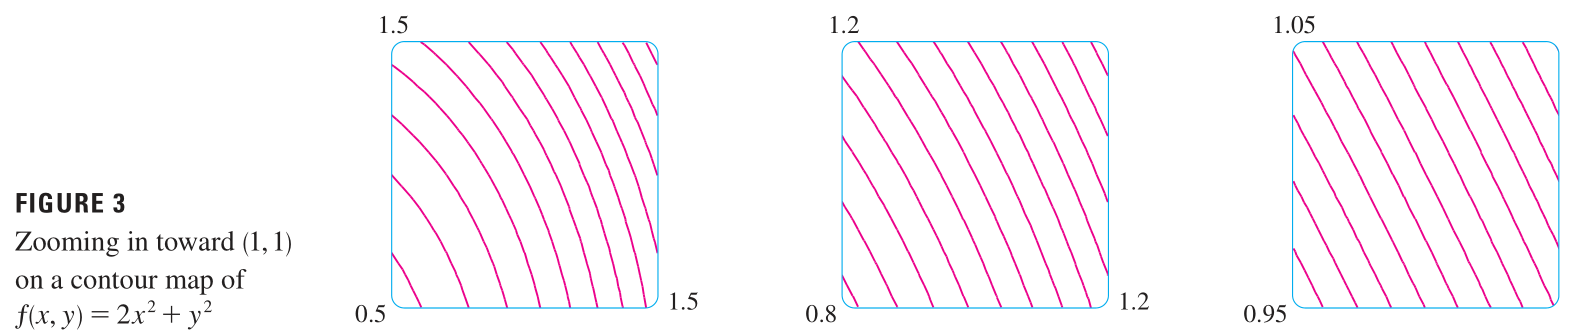
\includegraphics[width = 16 cm]{./images/tangent2.png } 
\end{center}

\begin{minipage}[]{0.54\linewidth}
\subsection*{{\fontfamily{lmss}\selectfont \underline{Linear Approximations}}}
The equation of the tangent plane of $f(x,y) = 2 x^2 + y^2 $ at the point (1, 1, 3) is $z = 4x + 2y - 3 $. Therefore, the linear function of 2 variables 
\[L(x,y) = 4x + 2y - 3 \]
is the \textit{linearization of f} at (1, 1) and the approximation 
\[f(x,y) \approx 4x + 2y - 3 \]
is the \textit{linear approximation} or \textit{tangent plane approximation} of $f$ at (1, 1).
\end{minipage} \hfill
\begin{minipage}[]{0.42\linewidth}
  \begin{mdframed}
Eg: At the point $(1.1,0.95)$, the linear approximation gives 
\[f(1.1,0.95) \approx 4(1.1) + 2(0.95) - 3 = 3.3\]
True value: $f(1.1, 0.95) = 2(1.1)^2 + (0.95)^2 = 3.3225$.
  \end{mdframed}
\end{minipage}

\begin{Def}[]
\textbf{\textcolor{blue5}{\fontfamily{lmss}\selectfont The linearization of $f$ at $(a,b)$.}} $L(x,y) = f(a,b) + f _ x (a,b) (x-a) + f _ y (a,b)(y-b)$\\
\textbf{\textcolor{blue5}{\fontfamily{lmss}\selectfont The linear approximation of $f$ at $(a,b)$.}} $f(x,y) \approx f(a,b) + f _ x (a,b) (x-a) + f _ y (a,b)(y-b)$
\end{Def}

\begin{minipage}[]{0.34\linewidth}
  \begin{center}
    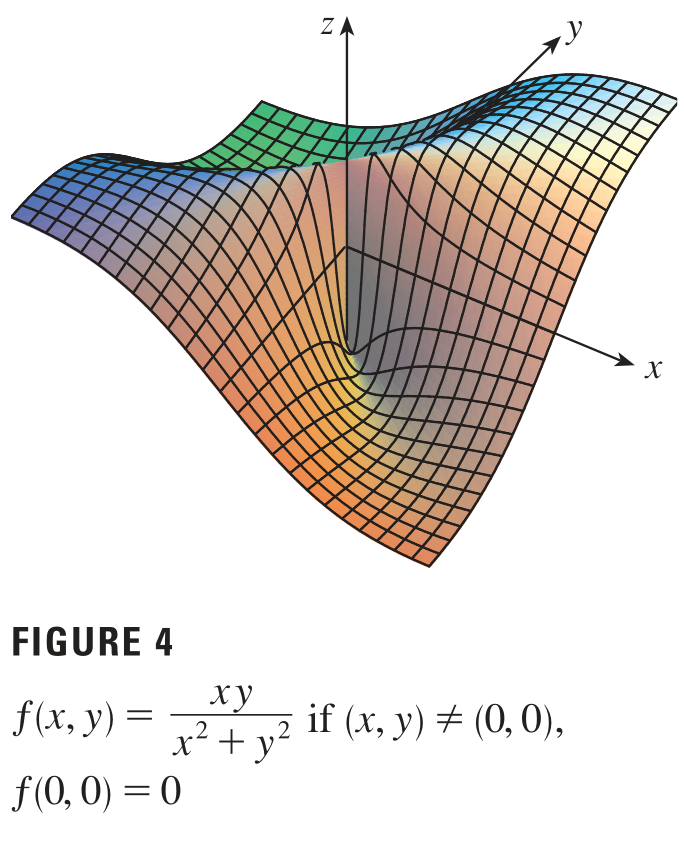
\includegraphics[width = 4.3 cm]{./images/linear.png}
    
  \end{center}
  
\end{minipage}
\begin{minipage}[]{0.63\linewidth}
What if $f _ x $ and $ f _ y $ are not continuous? 
\[f(x,y) = \begin{cases}
  \cfrac{xy }{x^2 + y^2 }& \text{ if } (x,y) \ne (0,0) \\
  0 & \text{ if } (x,y) = (0,0)
\end{cases}\]
Even though $f_x (0,0) = f_y (0,0) = 0$, but they are not continuous.
The linear approximation would be $f(x,y) \approx 0 $, but $f(x,y) = \frac{1 }{2 }$ at all points on the line $y = x $. So we define it as follow.
\end{minipage}

\pagebreak
\begin{Def}[Differentiable]
  If $z = f(x,y)$, then $f $ is \textbf{differentiable} at $(a,b)$ if $\Delta z $ can be expressed as 
  \[\Delta z = f_x (a,b) \Delta x + f_y(a,b) \Delta y + \varepsilon _1 \Delta x + \varepsilon _2 \Delta y \]
  where $\varepsilon _ 1 $ and $ \varepsilon _ 2 \to 0$ as $(\Delta x, \Delta y) \to (0,0)$ .
\end{Def}

\begin{mdframed}
  \textbf{\textcolor{blue5}{\fontfamily{lmss}\selectfont Theorem.}} If $f_x$ and $f_y $ exist near $(a,b)$ and are continuous at $(a,b)$, then $f $ is differentiable at $(a,b)$.
\end{mdframed}
\begin{minipage}[]{0.28\linewidth}
  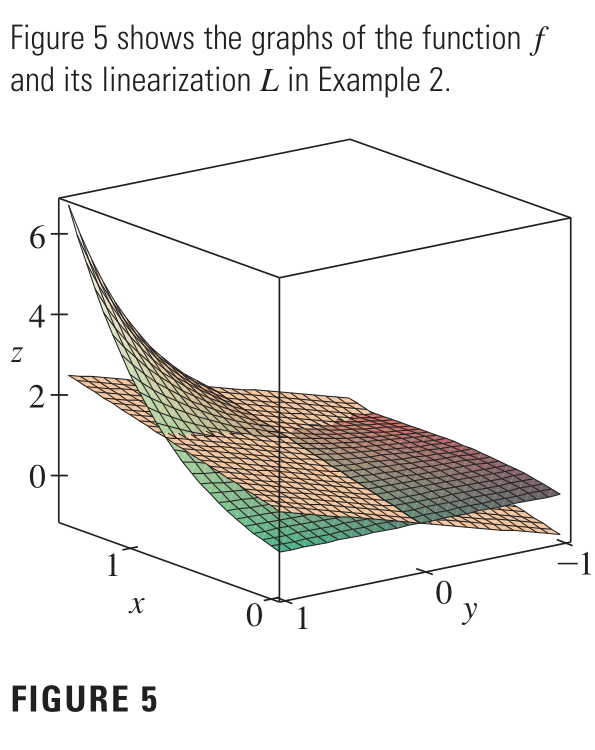
\includegraphics[width = 4.3 cm]{./images/leg2.png}
  
\end{minipage}\hfill
\begin{minipage}[]{0.69\linewidth}
  {\fontfamily{lmtt}\selectfont \textbf{\textcolor{blue5}{{\small \faIcon{map-marker-alt}} EXAMPLE.}}} Show that $f(x,y) = xe^{xy}$ is differentiable at  (1,0) and find its linearization there. Approximate f(1.1, -0.1).

  The partial derivatives are 
  \begin{align*}
    & f_x(x,y) = e^{xy} + x y e^{xy} & & f_x(x,y) = x^2 e^{xy} \\
    & f_x(1,0)  = 1 & & f_y(1,0) = 1
  \end{align*}  
  Both $f_x$ and $f_y $ are continuous, so by the above Theorem, we got $f$ differentiable. The linearization is 
  \begin{align*}
    L(x,y) & = f(1,0) + f_x (1,0)(x-1) + f _ y (1,0)(y - 0) \\
           & = x + y 
  \end{align*}
  So $f(1.1, -0,1) \approx 1.1 - 0.1 = 1 $, actual value: $0.98542 $.
\end{minipage}

\begin{minipage}[]{0.3\linewidth}
  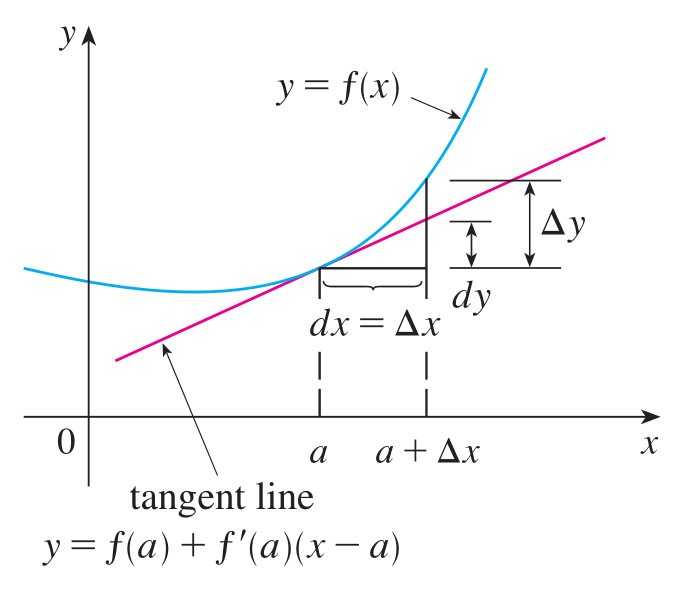
\includegraphics[width = 4.3 cm]{./images/tangentline.png}
\end{minipage}
\begin{minipage}[b]{0.67\linewidth}
\subsection*{{\fontfamily{lmss}\selectfont \underline{\textcolor{blue5}{Differentials}}}}
\textcolor{blue5}{$\blacksquare$} For $y = f(x)$, we define $dx$ an independent variable. And $dy = f'(x)\,dx$, represents the change in height when $x$ changes $dx$. 

\textcolor{blue5}{$\blacksquare$} For a differentiable $z  = f(x,y )$, we define the \textbf{differentials} $dx $ and $dy $ to be independent variables.


\end{minipage}

\begin{Def}[Total differential]
  
Then the \textbf{differential} $dz$ (the \textbf{total differential}), is defined as follow.
  \[dz = f_x(x,y)\,dx + f_y(x,y)\,dy = \cfrac{\partial z }{\partial x }\, dx + \cfrac{\partial z }{ \partial y }\, dy \]
\end{Def}
If we take $dx = \Delta x = x - a $ and $dy = \Delta y = y - b $, then $f(x,y) \approx f(a,b) + dz $.

\begin{center}
  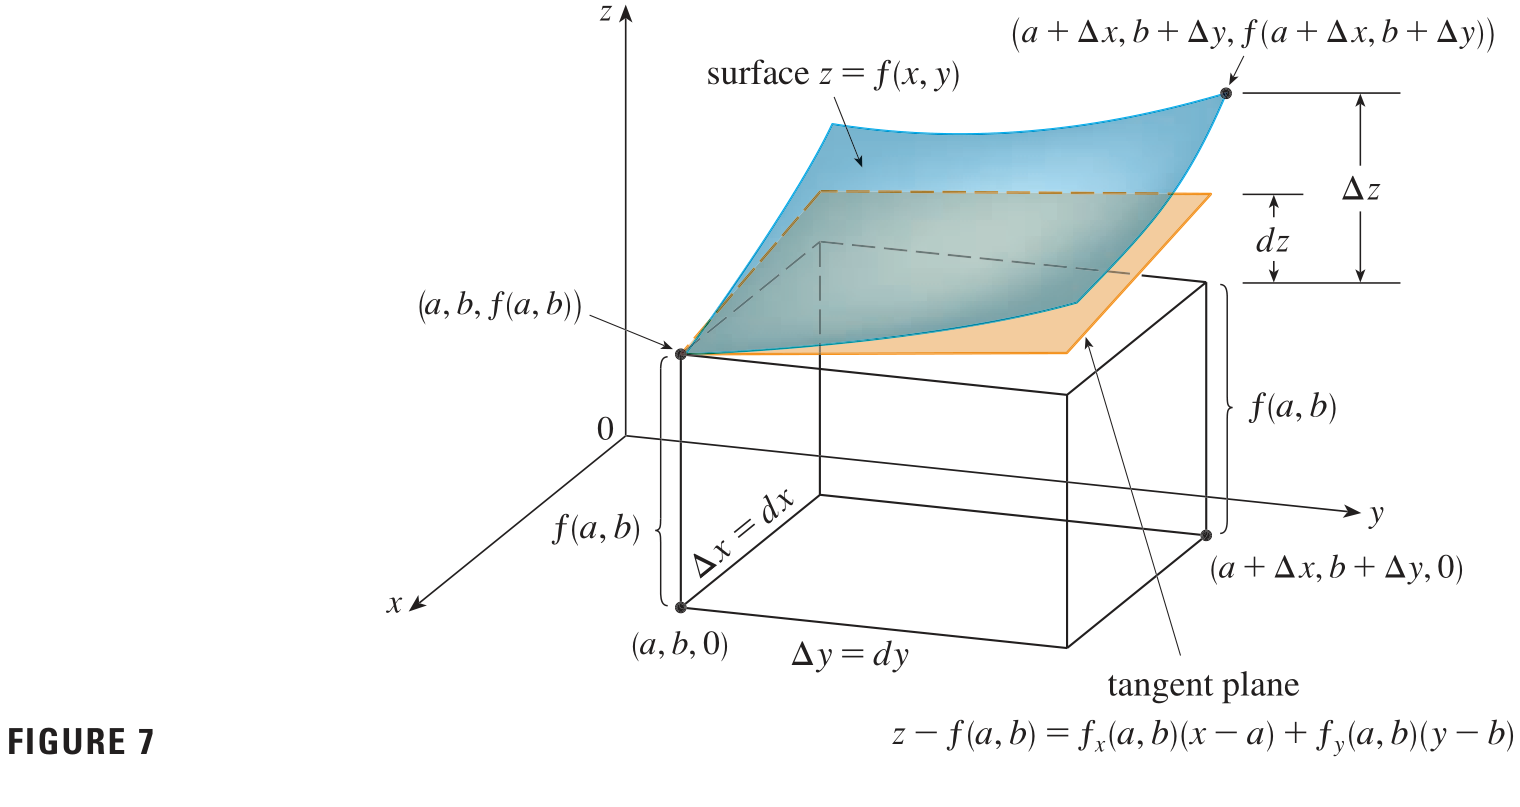
\includegraphics[width = 13 cm]{./images/tangentplaneapp.png} 
\end{center}

\begin{minipage}[]{0.3\linewidth}
  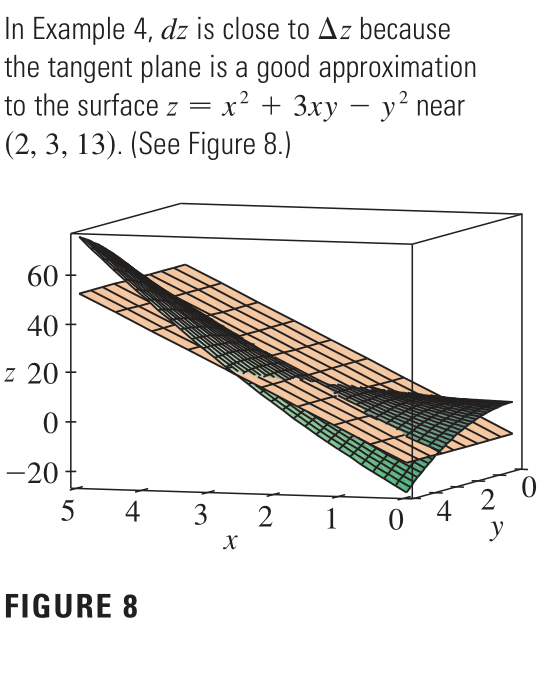
\includegraphics[width = 4.3 cm]{./images/fig8.png}
\end{minipage}
\begin{minipage}[]{0.64\linewidth}
  {\fontfamily{lmtt}\selectfont \textbf{\textcolor{blue5}{{\small \faIcon{map-marker-alt}} EXAMPLE.}}} \\
  (a) If $z = f(x,y) = x^2 + 3xy - y^2 $, find the differential $dz $.\\
  (b) If $x $ changes from 2 to 2.05 and $y $ changes from 3 to 2.96, comppare the values of $\Delta z $ and $dz$.

  \noindent
  {\fontfamily{lmtt}\selectfont \textbf{\textcolor{blue5}{SOLUTION}}} \\
  (a) Applying the formula, \[dz = \,dy = \cfrac{\partial z }{\partial x }\, dx + \cfrac{\partial z }{ \partial y }\, dy = (2x + 3y) \,dx + (3x - 2y)\,dy\]
  (b) Putting $x = 2, \,dx = \Delta x = 0.05, y = 3, dy = \Delta y = -0.04$, we get
  \[dz = [2(2) + 3 (3)]0.05 + [3(2) - 2(3)](-0.04) = 0.65\]
  The increment of $z $ is 
  \begin{align*}
    \Delta z & = f(2.05, 2.96) - f(2,3) \\
             & = [(2.05)^2 + 3(2.05)(2.96) - (2.96)^2] - [2^2 + 3(2)(3) - 3^2] \\
             &= 0.6449
  \end{align*}
{\small \faIcon{greater-than}}
Notice that $\Delta z \approx dz$ but $dz $ is easier to compute.

\end{minipage}

\subsection*{{\fontfamily{lmss}\selectfont \underline{Functions of Three or More Variables}}}
\textbf{Linear approximation.} $f(x,y,z) \approx f(a,b,c) + \Sigma f_x (a,b,c)(x-a)$ \\
\textbf{Total differential.} $dw = \cfrac{\partial w }{\partial x }\, dx + \cfrac{\partial w }{ \partial y }\, dy + \cfrac{\partial w }{\partial z } \,dz$

\section{The Chain Rule}
\begin{Def}[The Chain Rule (Case 1)]
  Suppose that $z = f(x,y)$ is differentiable, where $x = g(t)$ and $y = h(t)$ are both differentiable. Then $z $ is a differentiable function of $t $ and 
  \[\cfrac{dz}{dt } = \cfrac{\partial f }{ \partial x } \, \cfrac{dx }{dt } + 
  \cfrac{\partial f }{\partial y }\, \cfrac{dy }{ dt }\]
\end{Def}

\begin{minipage}[]{0.3\linewidth}
  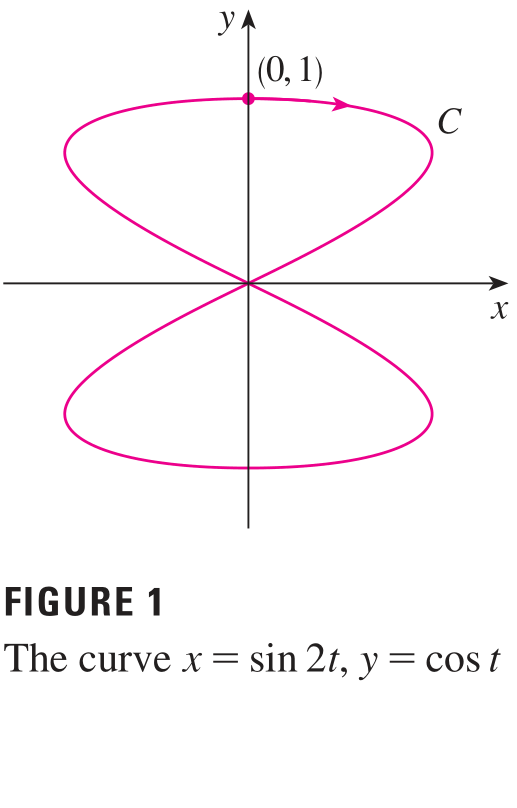
\includegraphics[width = 4.0 cm]{./images/sin2tcost.png}
  
\end{minipage}
\begin{minipage}[]{0.65\linewidth}
{\fontfamily{lmtt}\selectfont \textbf{\textcolor{blue5}{\faIcon{map-marker-alt} EXAMPLE.}}} 
If $z = x^2 y + 3x y^4 $, where $x = \sin{2t}$ and $y = \cos{t}$, find $dz/dt $ when $t = 0 $.

The Chain Rule gives 
\begin{align*}
  \cfrac{dz }{dt } & = \cfrac{\partial f }{ \partial x } \, \cfrac{dx }{dt } + \cfrac{\partial f }{\partial y }\, \cfrac{dy }{ dt } \\
                   & = (2xy + 3y^4)(2\cos{2t}) + (x^2 + 12xy^3)(-\sin{t})
\end{align*}
When $t = 0 $, $x = \sin{0} = 0$ and $y = \cos{0} = 1 $. Therefore 
\[\cfrac{dz }{dt } \Bigg|_{t = 0} = (0 + 3)(2 \cos{0}) + (0 + 0)(-0) = 6 \]
  
\end{minipage}

\begin{Def}[The Chain Rule (Case 2)]
  Suppose that $z = f(x,y)$ is differentiable, where $x = g(s,t)$ and $y = h(s,t)$ are differentiable. We can hold the the other variable fixed.
  \[\cfrac{dz}{ds } = \cfrac{\partial f }{ \partial x } \, \cfrac{dx }{ds } + \cfrac{\partial f }{\partial y }\, \cfrac{dy }{ ds } \quad \text{ } \quad \cfrac{dz}{dt } = \cfrac{\partial f }{ \partial x } \, \cfrac{dx }{dt } + 
  \cfrac{\partial f }{\partial y }\, \cfrac{dy }{ dt }\]
\end{Def}
{\fontfamily{lmtt}\selectfont \textbf{\textcolor{blue5}{\faIcon{map-marker-alt} EXAMPLE.}}} If $z = e^x \sin{y}$, where $x = st^2$, and $y = s^2 t $, find $\partial z/ \partial s $ and $ \partial z / \partial t $.

Applying Case 2 of the Chain Rule, we get 
\begin{align*}
  \cfrac{\partial z }{\partial s } & = \cfrac{\partial f }{ \partial x } \, \cfrac{\partial x }{\partial s } + \cfrac{\partial f }{\partial y }\, \cfrac{\partial y }{ \partial s } = (e^x \sin{y})(t^2) + (e^x \cos{y})(2st) \\
                                   & = t^2 e^{st^2} \sin{(s^2t)} + 2ste^{st^2}\cos{(s^2t)} \\
  \cfrac{\partial z }{\partial t } & = \cfrac{\partial f }{ \partial x } \, \cfrac{\partial x }{\partial t } + \cfrac{\partial f }{\partial y }\, \cfrac{\partial y }{ \partial t } = (e^x \sin{y})(2st) + (e^x \cos{y})(s^2) \\
                                   & = 2ste^{st^2} + s^2 e^{st^2}\cos{s^2t}
\end{align*}

\begin{minipage}[]{0.28\linewidth}
 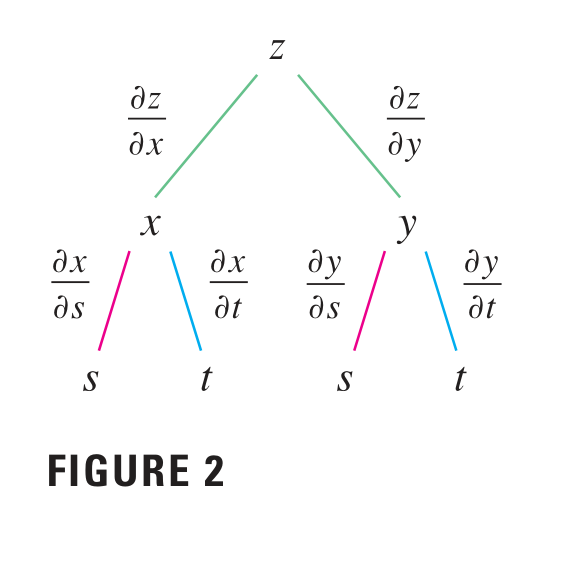
\includegraphics[width = 4 cm]{./images/dxyzt.png}
  
\end{minipage}
\begin{minipage}[]{0.69\linewidth}
\textcolor{purple}{\faIcon{greater-than} \textbf{{\fontfamily{lmtt}\selectfont Note.}}}
 $s, t $ are \textbf{independent} variables, $x, y $ are \textbf{intermediate} variables, and $z $ is the \textbf{dependent} variable.

 For the gemeral version of $n$ variables, it's similar.

  
\end{minipage}\\
{\fontfamily{lmtt}\selectfont \textbf{\textcolor{blue5}{\faIcon{map-marker-alt} EXAMPLE.}}} If $g(s,t) = f(s^2 - t^2, t^2 - s^2 )$ and $f $ is differentiable, show that $g $ satisfies the equation  \[t \,\cfrac{\partial g }{ \partial s } + s \, \cfrac{\partial g }{ \partial t } = 0\]
{\fontfamily{lmtt}\selectfont \textbf{\textcolor{blue5}{\faIcon{map-marker-alt} EXAMPLE.}}} If $z = f(x,y)$ has continuous second-order partial derivatives and $x = r^2 + s^2 $ and $ y = 2 rs $, find \\
\textbf{a.} $\partial z / \partial r$ \\
\textbf{b.} $\partial ^2 z / \partial r^2 $ \\
{\fontfamily{lmtt}\selectfont \textbf{\textcolor{blue5}{SOLUTION.}}} \\
\textbf{a.} The Chain Rule gives 
\[ \cfrac{\partial z }{\partial r }  = \cfrac{\partial f }{ \partial x } \, \cfrac{\partial x }{\partial r } + \cfrac{\partial f }{\partial y }\, \cfrac{\partial y }{ \partial r } = \cfrac{\partial z }{ \partial x } (2r) + \cfrac{\partial  z }{ \partial y } (2s )\]

\textbf{b.} Applying the Product Rule, we get 
\begin{align*}
  \cfrac{\partial ^2 z }{\partial r^2 } & = \cfrac{\partial }{\partial r } \left( 2r \cfrac{\partial z }{\partial x } + 2s \cfrac{\partial z }{\partial y } \right) \\
  & = 2 \cfrac{\partial z }{\partial x } + 2r \cfrac{\partial }{\partial r } \left( \cfrac{\partial z }{\partial x } \right) + 2s \cfrac{\partial }{\partial r } \left( \cfrac{\partial z }{\partial y } \right)
\end{align*}

\begin{minipage}[]{0.26\linewidth}
  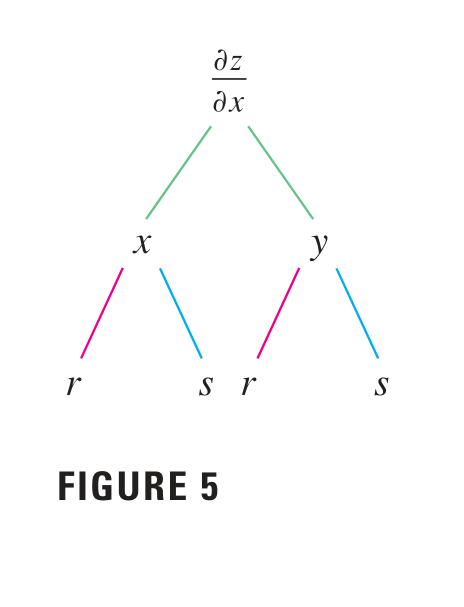
\includegraphics[width = 4 cm]{./images/chainrulefig5.png}
  
\end{minipage}
\begin{minipage}[]{0.69\linewidth}

Using the Chain Rule again (Figure 5), we have 
\begin{align*}
  \cfrac{\partial  }{\partial r  } \left( \cfrac{\partial z }{ \partial x } \right) = \cfrac{\partial }{ \partial x } \left( \cfrac{\partial z }{ \partial x } \right) \cfrac{\partial x }{ \partial r } + \cfrac{\partial }{ \partial y } \left( \cfrac{\partial z }{ \partial x } \right) \cfrac{\partial y }{\partial r }= \cfrac{\partial ^2 z }{\partial x^2 } (2r) + \cfrac{\partial ^2 z }{\partial y \partial x } (2s) \\
  \cfrac{\partial }{ \partial r } \left( \cfrac{\partial z }{ \partial y } \right) = \cfrac{\partial ^2 z }{\partial x \partial y } (2r) + \cfrac{\partial ^2 z }{ \partial y^2 }(2s) 
\end{align*} 
\end{minipage}\\
Putting these into the previous equation, 
\[\cfrac{\partial ^2 z }{\partial r^2 } = 2 \cfrac{\partial z }{\partial x } + 4 r^2 \cfrac{dd^2 z }{\partial x^2 } + 8rs \cfrac{\partial ^2 z }{\partial x \partial y } + 4s^2 \cfrac{\partial ^2 z }{\partial y^2 }\]

\subsection*{{\fontfamily{lmss}\selectfont \underline{Implicit Differentiation}}}
Suppose $F(x,y) = 0 $, $y = f(x)$ is differentiable. If $F $ is differentiable, apply Case 1 of the Chain Rule to differentiate both sides with respect to $x $.
\[\cfrac{\partial F }{\partial x } \cfrac{dx }{ dx } + \cfrac{\partial F }{ \partial y } \cfrac{dy }{dx } = 0\]
\begin{center}
  \begin{minipage}[]{0.3\linewidth}
    \begin{mdframed}
      \[\cfrac{dy }{dx } = - \cfrac{\cfrac{\partial F }{\partial x }}{\cfrac{\partial F }{ \partial y }} = - \cfrac{F_x }{F_y}\]
    \end{mdframed}
  \end{minipage}
\end{center}
{\fontfamily{lmtt}\selectfont \textbf{\textcolor{blue5}{\faIcon{map-marker-alt} EXAMPLE.}}} Find $y' $ if $x^3 + y^3 = 6xy $.

{\fontfamily{lmtt}\selectfont \textbf{\textcolor{blue5}{SOLUTION.}}} $F(x,y) = x^3 + y^3 - 6xy = 0 $ which gives 
\[\cfrac{dy }{dx } = -\cfrac{F_x }{F_y } = - \cfrac{3x^2 - 6y }{3y^2 - 6x } = - \cfrac{x^2 - 2y }{y^2 - 2x }\]

\begin{Def}[Implicit Function Theorem]
  \[\cfrac{\partial z }{\partial x } = - \cfrac{\cfrac{\partial F }{ \partial x }}{\cfrac{\partial F }{\partial z }} \quad \text{ } \quad \cfrac{\partial z }{\partial y } = - \cfrac{\cfrac{\partial F }{\partial y }}{\cfrac{\partial F }{\partial z }}\]
\end{Def}
{\fontfamily{lmtt}\selectfont \textbf{\textcolor{blue5}{\faIcon{map-marker-alt} EXAMPLE.}}} Find $\cfrac{\partial z }{ \partial x }$ and $ \cfrac{\partial z }{\partial y }$ if $x^3 + y ^3 + z^3 + 6xyz = 1 $.

{\fontfamily{lmtt}\selectfont \textbf{\textcolor{blue5}{SOLUTION.}}} 
Let $f(x,y,z) = x^3 + y^3 + z^3 + 6xyz - 1 $, then we have 
\begin{align*}
  \cfrac{\partial z }{ \partial x } = - \cfrac{F_x }{F_z } = - \cfrac{x^2 + 2yz }{z^2 + 2xy } \\
  \cfrac{\partial z }{ \partial y } = - \cfrac{F_y }{F_z } = - \cfrac{y^2 + 2xz }{z^2 + 2xy }
\end{align*}

\section{Directional Derivatives and the Gradient Vector}

\begin{minipage}[]{0.5\linewidth}
  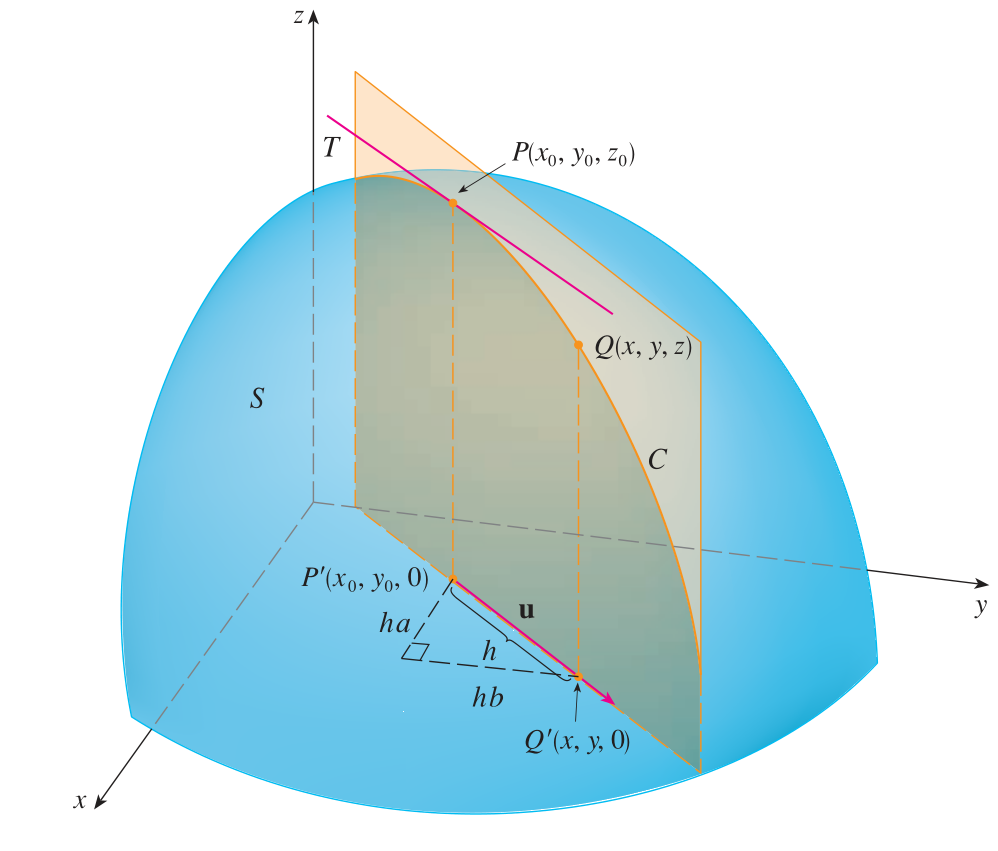
\includegraphics[width = 8 cm]{./images/grad.png}
  
\end{minipage}
\begin{minipage}[]{0.47\linewidth}
\subsection*{{\fontfamily{lmss}\selectfont \textcolor{blue5}{\faIcon{anchor} \underline{Directional Derivatives}}}}
We want the rate of change of $z$ at $(x _ 0, y _ 0 )$ in the direction of an unit vector \textbf{u} = $\langle a, b  \rangle$. 

\textcolor{blue5}{\faIcon{caret-right}} Consider the surface $S$ of $z = f(x,y)$, the vertical plane that passes through $P(x_0, y_0, z_0)$  in the direction of \textbf{u} intersects $S$ a curve $C$. 

\textcolor{blue5}{\faIcon{caret-right}} The slope of tangent line $T$ to $C$ at $P$ is what we need.
\end{minipage}

If $Q(x,y,z)$ is another point on $C$ and $P', Q'$ are the projections of $P, Q$ onto the $xy$-plane, then the vector $\vv{P'Q'}$ is parallel to \textbf{u}, 
\[\vv{P'Q'} = h \textbf{u} = \langle ha, hb  \rangle  \]
Therefore $x - x_0 = ha$, $y - y_0 = hb $.
\[ \cfrac{\Delta z }{h } = \cfrac{z - z_0 }{h } = \cfrac{f(x_0 + ha, y_0 + hb ) - f(x_0, y_0)}{h}\]
If we take limit as $h \to 0 $, we obtain the rate of change of $z $ (with respect to distance) in the direction of \textbf{u}.
\begin{Def}[Directional Derivatives]
  The \textbf{directional derivative} of $f $ at $(x_0, y_0 )$ in the direction of a unit vector \textbf{u} = $\langle a, b  \rangle$ is 
  \begin{align*}
    D_u f(x_0, y_0 ) & = \lim_{h \to 0 }\cfrac{f(x_0 + ha, y_0 + hb ) - f(x_0, y_0)}{h} \\
                     & = f_x(x,y) a + f_y (x,y) b \\
                     & = f_x(x,y) \cos{\theta} + f_y(x,y) \sin{\theta}  \quad \text{(\textbf{u} makes an angle $\theta$ with the $x^{+}$-axis)} 
  \end{align*}    
\end{Def}

\begin{minipage}[]{0.3\linewidth}
  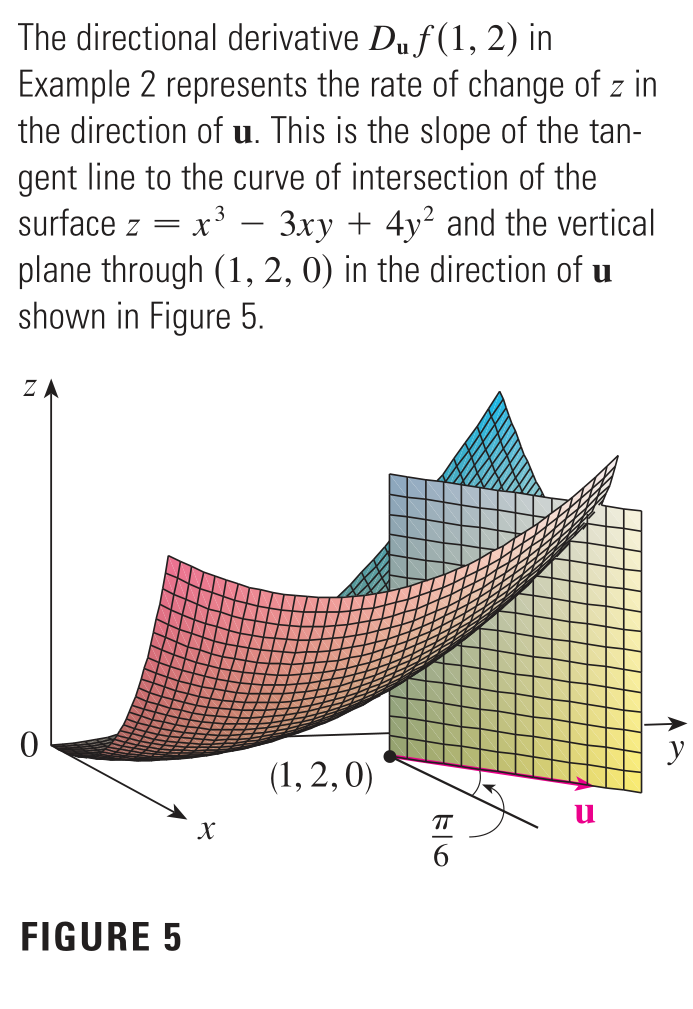
\includegraphics[width = 4.7 cm]{./images/grad2.png}
  
\end{minipage}
\begin{minipage}[]{0.67\linewidth}
{\fontfamily{lmtt}\selectfont \textbf{\textcolor{blue5}{\faIcon{map-marker-alt} EXAMPLE.}}} Find the directional derivative $D_uf(x,y)$ if \[f(x,y) = x^3 - 3xy + 4 y^2 \]
and \textbf{u} is given by $\theta = \pi/6$. What is $D_ \textbf{u} f(1,2)$?
 
{\fontfamily{lmtt}\selectfont \textbf{\textcolor{blue5}{SOLUTION.}}}  
$  f_x(x,y) = 3 x^2 - 3y \quad \text{ } \quad  f_y(x,y) = 8y -3 $

Therefore, 
\begin{equation*}
  \begin{split}
D_u f(x,y)  & = \cfrac{\sqrt{3 }}{2}(3 x^2 - 3y) + \cfrac{1 }{2 } (8y - 3)  \\
& = \cfrac{3 \sqrt{3 }}{2 } x^2 + \cfrac{4 - 3 \sqrt{3 }}{2 } y - \cfrac{3 }{ 2 }
  \end{split}
\end{equation*}
Hence $D_u f(1,2) = \cfrac{13 - 3 \sqrt{3 }}{2 }$
\end{minipage}
\pagebreak
\subsection*{{\fontfamily{lmss}\selectfont \textcolor{blue5}{\faIcon{anchor} \underline{The Gradient Vector}}}}
Notice that $D_ \textbf{u} = \langle f_x(x,y) , f_y(x,y) \rangle \cdot \textbf{u}$.
\begin{Def}[Gradient]
  The \textbf{gradient} of $f(x,y)$ is the vector function $\nabla f$ defined by 
  \[\nabla f(x,y) = \langle f_x (x,y) , f_y(x,y) \rangle = \cfrac{\partial f }{ \partial x } \textbf{i} + \cfrac{\partial f }{\partial y } \textbf{j}\]
  The directional derivative of $f(x,y)$ is $\quad D_ \textbf{u} f(x,y) = \nabla f(x,y) \cdot \textbf{u}$
\end{Def}
{\fontfamily{lmtt}\selectfont \textbf{\textcolor{blue5}{\faIcon{map-marker-alt} EXAMPLE.}}} If $f(x,y) = \sin{x} + e^{xy}$, then 
\begin{align*}
  & \nabla f(x,y) = \langle f_x, f_y  \rangle = \langle \cos{x} + y e^{xy}, xe^{xy} \rangle \\
  & \nabla f(0,1) = \langle 2, 0  \rangle
\end{align*}

\begin{minipage}[]{0.3\linewidth}
  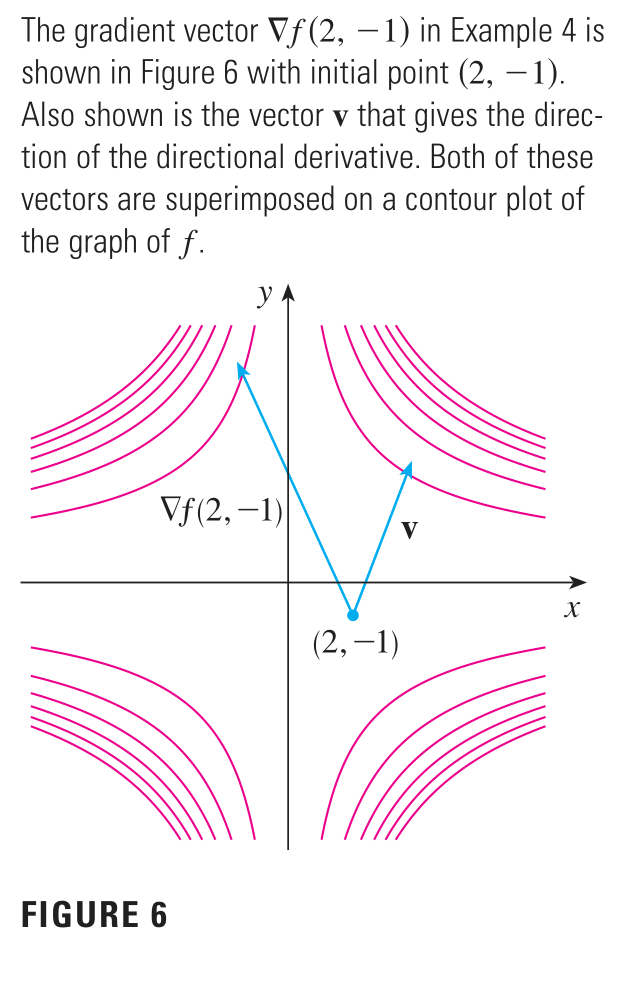
\includegraphics[width = 4.3 cm]{./images/grad4.png}
  
\end{minipage}
\begin{minipage}[]{0.67\linewidth}
  {\fontfamily{lmtt}\selectfont \textbf{\textcolor{blue5}{\faIcon{map-marker-alt} EXAMPLE.}}} Find the directional derivative of $f(x,y) = x^2 y^3 - 4y$ at $(2, -1 )$ in the direction of $\textbf{v} = 2 \textbf{i} + 5 \textbf{j}$.

  {\fontfamily{lmtt}\selectfont \textbf{\textcolor{blue5}{SOLUTION.}}} We first compute the gradient vector at $(2,-1)$: 
  \begin{align*}
    \nabla f(x,y) & = 2xy^3 \textbf{i} + (3 x^2 y^2 - 4 ) \textbf{i} \\
    \nabla f(2, -1) & = -4 \textbf{i} + 8 \textbf{j}
  \end{align*}
  The unit vector in the direction of \textbf{v} is $\textbf{u} = \cfrac{\textbf{v}}{|\textbf{v}|} = \cfrac{2 }{\sqrt{29 }} \textbf{ i} + \cfrac{5 }{\sqrt{29 }} \textbf{ j}$

  Therefore we have 
  \begin{align*}
    D_ \textbf{u} f(2,-1) & = \nabla f(2,-1) \cdot \textbf{u} = (-4 \textbf{i} + 8 \textbf{j}) \cdot \left( \cfrac{2 }{\sqrt{29 }} \textbf{ i} + \cfrac{5 }{\sqrt{29 }} \textbf{ j}  \right)\\
    & = \cfrac{-4 \cdot 2 + 8 \cdot 5  }{\sqrt{29}} = \cfrac{32 }{\sqrt{29 }}
  \end{align*}
\end{minipage}

\subsection*{{\fontfamily{lmss}\selectfont \textcolor{blue5}{\faIcon{anchor} \underline{Functions of Three Variables}}}}
\begin{Def}[Directional Derivatives]
  The \textbf{directional derivative} of $f$ at $(x_0, y_0, z_0)$ in the direction of a unit vector \textbf{u} $= \langle a, b, c  \rangle$ is 
  \[D_ \textbf{u} f(x_0, y_0, z_0) = \lim_{h \to 0 } \cfrac{f(x_0 + ha, y_0 + hb, z_0 + hc ) - f(x_0, y_0, z_0)}{h}\]
  The \textbf{gradient vector} is 
  \[\nabla f = \langle f_x, f_y, f_z  \rangle = \cfrac{\partial f }{ \partial x } \textbf{ i} + \cfrac{\partial f }{\partial y } \textbf{ j} + \cfrac{\partial f }{\partial z } \textbf{ k}  \]
  And the directional derivative is $\quad D_ \textbf{u} f(x,y,z) = \nabla f(x,y,z) \cdot \textbf{u}$
\end{Def} 
{\fontfamily{lmtt}\selectfont \textbf{\textcolor{blue5}{\faIcon{map-marker-alt} EXAMPLE.}}} If $f(x,y,z) = x \sin{yz}$, (a) find $\nabla f$ and (b) find $D_ \textbf{u} f(1,3,0)$ in the direction of $\textbf{v} = \textbf{i} + 2 \textbf{j}  - \textbf{k}$.

{\fontfamily{lmtt}\selectfont \textbf{\textcolor{blue5}{SOLUTION.}}} 
\[\nabla f = \sin{yz} \cdot \textbf{i} + xz\cos{yz} \cdot \textbf{j} + xy\cos{xz} \cdot \textbf{k}\]
The unit vector in the direction of \textbf{v} is 
\[\textbf{u} = \cfrac{1 }{\sqrt{6 }} \textbf{i} + \cfrac{2 }{\sqrt{6 }} \textbf{j} - \cfrac{1 }{\sqrt{6 }} \textbf{k}\]
Therefore 
\begin{align*}
  D _ \textbf{u} & = \nabla f(1,3,0) \cdot \textbf{u} \\
  & = 3 \textbf{k} \cdot \cfrac{1 }{\sqrt{6 }} \textbf{i} + \cfrac{2 }{\sqrt{6 }} \textbf{j} - \cfrac{1 }{\sqrt{6 }} \textbf{k} \\
  & = - \sqrt{\cfrac{3 }{2 }}
\end{align*}

\subsection{Maximizing the Directional Derivative}
\begin{Def}[Maximum Value of the Directional Derivative]
 The maximum value of $D_ \textbf{u} f(\textbf{x})$ is $|\nabla f(\textbf{x})|$, when \textbf{u} has the same direction as the gradient vector $\nabla f(\textbf{x})$.
\end{Def}

\begin{minipage}[]{0.3\linewidth}
  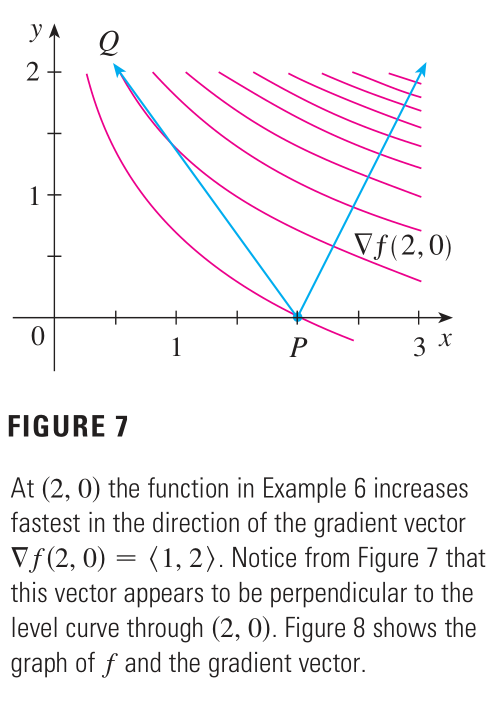
\includegraphics[width = 4.3 cm]{./images/maxeg6.png}
  
\end{minipage}
\begin{minipage}[]{0.67\linewidth}
  {\fontfamily{lmtt}\selectfont \textbf{\textcolor{blue5}{\faIcon{map-marker-alt} EXAMPLE.}}} 

  (a) If $f(x,y) = xe^y $, find the rate of change of $f$ at $P(2,0)$ in the direction from $P$ to $Q(\frac{1}{2}, 2 )$.

  (b) In what direction, $f$ has max $D _ \textbf{u} f$ and what's it?

  {\fontfamily{lmtt}\selectfont \textbf{\textcolor{blue5}{SOLUTION.}}} 

  (a) \begin{align*}
    \nabla f(x,y) & = \langle f_x, f_y  \rangle = \langle e^y, xe^y  \rangle \\
    \nabla f(2,0) & = \langle 1,2  \rangle
  \end{align*}
  The unit vector in the direction $\overrightarrow{PQ}$ is \textbf{u} $= \left< -\frac{3 }{5 }, \frac{4 }{5 }  \right>$, so we have 
  \begin{align*}
    D _ \textbf{u} f(2,0) & = \nabla f(2,0) \cdot \textbf{u} = \langle 1,2 \rangle \cdot  \left< -\frac{3 }{5 }, \frac{4 }{5 }  \right>  \\
    & = 1 \left( - \frac{3 }{5 } \right) + 2 \left( \frac{4 }{ 5 } \right) = 1
  \end{align*}

  (b) $f$ increases fastest in the direction of $\nabla f(2,0) = \langle 1, 2  \rangle$.
  \[|\nabla f(2,0)| = |\langle 1,2 \rangle  | = \sqrt{5 }\]
\end{minipage}

\subsection*{{\fontfamily{lmss}\selectfont \textcolor{blue5}{\faIcon{anchor} \underline{Tangent Planes to Level Surfaces}}}}

Suppose $S$ of $F(x,y,z) = k $, and $P(x_0, y_0, z_0) \in S$. We can write $\nabla F \cdot \textbf{r}'(t) = 0$ 
\[\nabla F (x_0, y_0, z_0) \cdot \textbf{r}'(t_0) = 0 \]
We see that the \textit{gradient vector} $\nabla F(x_0, y_0, z_0)$ is \textbf{perpendicular} to the tangent vector to any curve $C$ on $S$ that pass through $P$.

\begin{Def}[Tangent plane]
  If $\nabla F(x_0, y_0, z_0) \ne \textbf{0} $, there is a \textbf{tangent plane to the level surface $F(x,y,z) = k$ at $P(x_0, y_0, z_0)$} 
  \[F_x (x_0, y_0, z_0)(x - x_0) + F_y (x_0, y_0, z_0) ( y - y_0)  + F_z (x_0, y_0, z_0)(z - z_0)  = 0 \]
  The \textbf{normal line} to $S$ at $P$ is the line passing through $P$ and perpendicular to the tangent plane. The direction of it is given by $\nabla F(x_0, y_0, z_0)$ and its symmetric equation*s are 
  \[\cfrac{x - x_0 }{F_x (x_0, y_0, z_0)} = \cfrac{y - y_0 }{F_y (x_0, y_0, z_0)} = \cfrac{z - z_0 }{F_z (x_0, y_0, z_0)}\]
\end{Def}
{\fontfamily{lmtt}\selectfont \textbf{\textcolor{blue5}{{\small \faIcon{chevron-circle-right}} Special case.}}} When $z = f(x,y)$, then $F(x,y,z) = f(x,y) - z = 0$, we have 
\[f_x(x_0, y_0)(x - x_0) + f_y(x_0, y_0)(y - y_0) - (z - z_0) = 0\]
{\fontfamily{lmtt}\selectfont \textbf{\textcolor{blue5}{\faIcon{map-marker-alt} EXAMPLE.}}} Find the tangent plane and normal line at $(-2,1,-3)$ to the ellipsoid
\[\cfrac{x^2 }{4} + y^2 + \cfrac{z^2 }{9 } = 3 \]
{\fontfamily{lmtt}\selectfont \textbf{\textcolor{blue5}{SOLUTION.}}} The ellipsoid is the level surface ($k = 3 $) of the function 
\[F(x,y,z) = \cfrac{x^2 }{4 } + y^2 + \cfrac{z^2 }{9 }\]
Therefore we have 
\begin{align*}
  F_x(x,y,z) = \cfrac{x }{ 2 } & \quad & F_y(x,y,z) = 2y & \quad & F_z(x,y,z) = \cfrac{2z }{9 } \\
  F_x(-2, 1, -3 ) = -1 & \quad & F_y(-2, 1, -3)  = 2 & \quad & F_z(-2,1,-3) = - \cfrac{2 }{3 }
\end{align*}

\begin{minipage}[]{0.3\linewidth}
  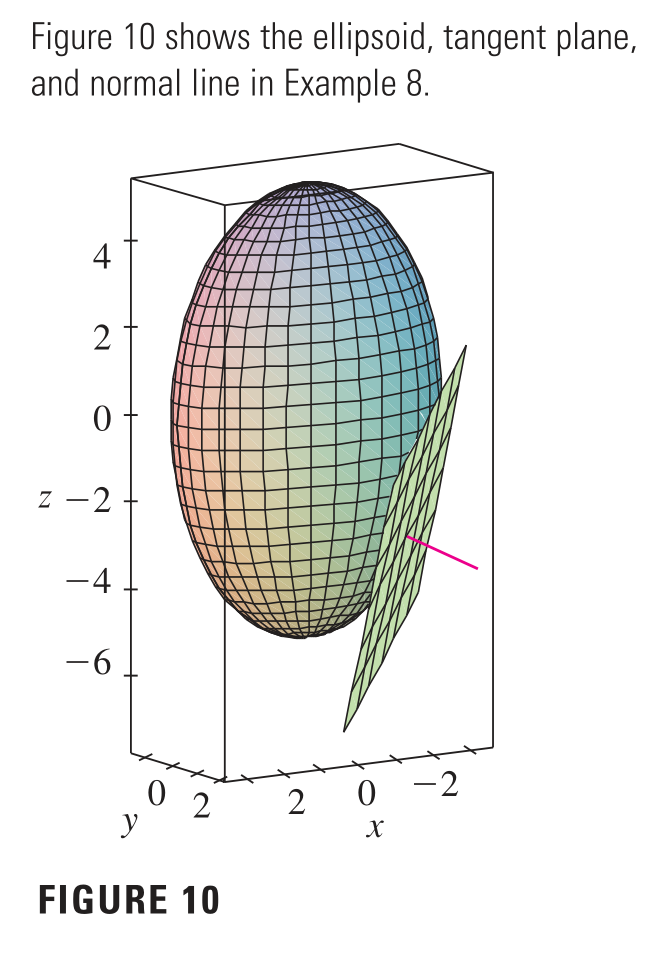
\includegraphics[width = 4.3 cm]{./images/fig10.png}
  
\end{minipage}
\begin{minipage}[]{0.67\linewidth}
The equation of the tangent plane at (-2, 1, -3) is 
\[-1(x + 2) + 2(y-1) - \cfrac{2}{3} (z + 3  ) = 0\]
The symmetric equations of the normal line are 
\[\cfrac{x + 2 }{ -1 } =  \cfrac{y - 1 }{2 } = \cfrac{z + 3 }{- \frac{2 }{3 }}\]
  
\end{minipage}

% \subsection*{{\fontfamily{lmss}\selectfont \textcolor{blue5}{\faIcon{anchor} \underline{Significance of the Gradient Vector}}}}
% Consider $f(x,y)$ and $P(x_0,y_0)$. Again $\nabla f(x_0, y_0)$ gives the direction of fastest increase of $f$. 

  \begin{minipage}[]{0.67\linewidth}
\subsection*{{\fontfamily{lmss}\selectfont \textcolor{blue5}{\faIcon{anchor} \underline{Maximum and Minimum Values}}}}
\begin{Def}[Local extrema]
\textbf{Local maximum} $f(a,b)$ if $f(x,y) \le f(a,b)$ when $(x,y)$ is near $(a,b)$.And the first-order partial derivatives of $f$ exists there, then $f_x(a,b) = 0$ and $f_y(a,b) = 0 $. 
\end{Def}
  
\end{minipage}
\begin{minipage}[]{0.3\linewidth}
  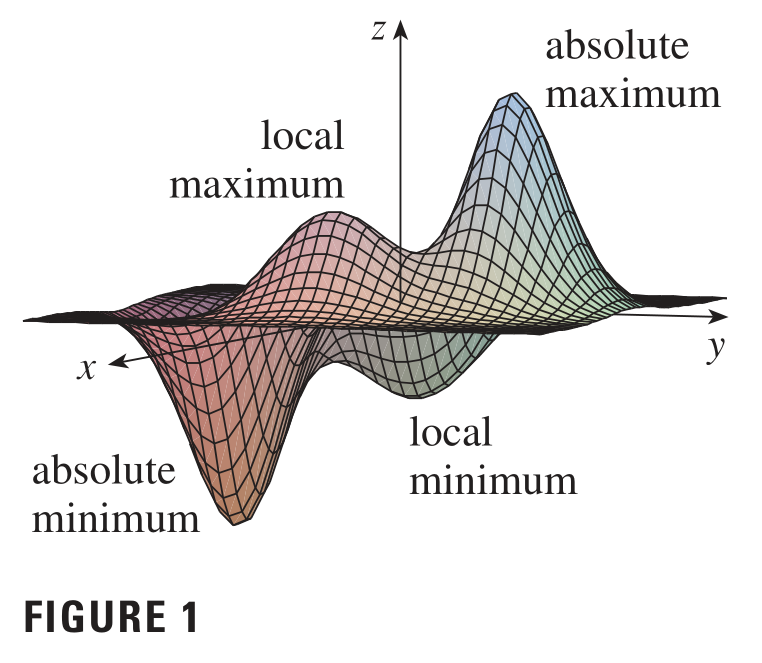
\includegraphics[width = 4.3 cm]{./images/localextrema.png}
  
\end{minipage}

If we put $f_x(a,b) = 0  $ and $f_y(a,b) = 0 $ in the equation of a tangent plane, we get $z = z_0$. So the tangent plane at a local extrema must be \textit{horizontal}.
A point $(a,b)$ is a \textbf{critical point} (or \textit{stationary point})  of $f$ if $f_x(a,b) = f_y(a,b) = 0$, or if one of these does not exist.

\begin{minipage}[]{0.3\linewidth}
  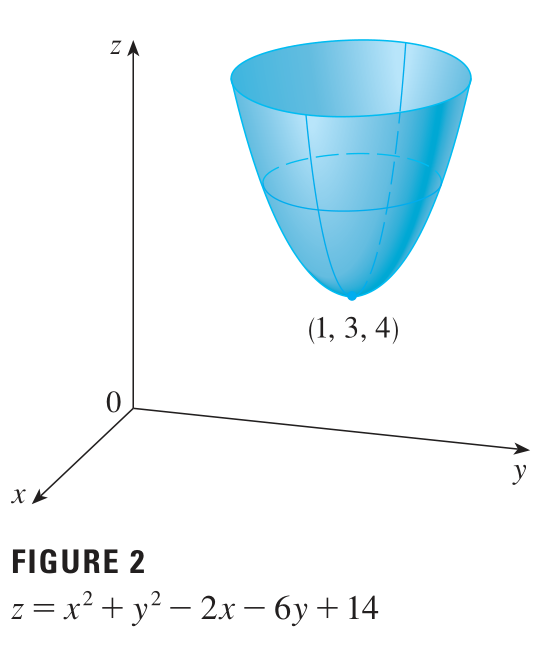
\includegraphics[width = 4.3 cm]{./images/min1}
  
\end{minipage}
\begin{minipage}[]{0.67\linewidth}

{\fontfamily{lmtt}\selectfont \textbf{\textcolor{blue5}{\faIcon{map-marker-alt} EXAMPLE.}}} Let $f(x,y) = x^2 + y^2 -2x - 6y + 14 $. Then 
\[f_x(x,y) = 2x - 2 \quad \text{ } \quad f_y(x,y) = 2y - 6 \]
These derivatives are equal to 0 when $x = 1, y = 3$. So the only critical point is $(1,3)$. 
\[f(x,y) = 4 + (x-1)^2 + (y-3)^2\]
We have $f(x,y) \ge 4 $. Therefore $f(1,3) = 4$ is a local minimum, and in fact it is the \textbf{absolute minimum} of $f$.
  
\end{minipage}

\begin{minipage}[]{0.3\linewidth}
  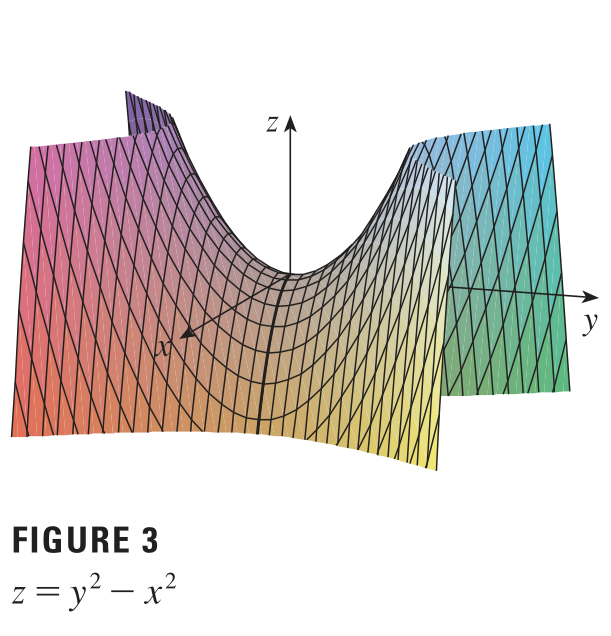
\includegraphics[width = 4.3 cm]{./images/saddle.png}
  
\end{minipage}
\begin{minipage}[]{0.67\linewidth}
  {\fontfamily{lmtt}\selectfont \textbf{\textcolor{blue5}{\faIcon{map-marker-alt} EXAMPLE.}}} Find the extreme values of $f(x,y) = x^2 + y^2 $.

 $f(x,y)$ is either maxima or minima depends on directions. So $(0,0)$ is a \textit{saddle point} of $f$. Then how to determine?
\end{minipage}

\begin{Def}[Second Derivatives Test]
  Suppose $f_x(a,b) = f_y(a,b) = 0 $. Let 
  \begin{align*}
  D & = D(a,b) = f_{xx}(a,b)f_{yy}(a,b) - [f_{xy}(a,b)]^2 \\
    & = \begin{vmatrix}
      f_{xx} & f_{xy} \\ 
      f_{yx} & f_{yy}
    \end{vmatrix} = f_{xx}f_{yy} - (f_{xy})^2
  \end{align*}
  (a) \textbf{Local minimum:} $D > 0, f_{xx}(a,b) > 0$.\\
  (b) \textbf{Local maximum:} $D > 0, f_{xx}(a,b) < 0$.\\
  (c) \textbf{Neither:} $D < 0$.
\end{Def}
{\fontfamily{lmtt}\selectfont \textbf{\textcolor{blue5}{\faIcon{greater-than} Note.}}} If $D = 0$, we have no idea.

\pagebreak

\begin{minipage}[]{0.3\linewidth}
  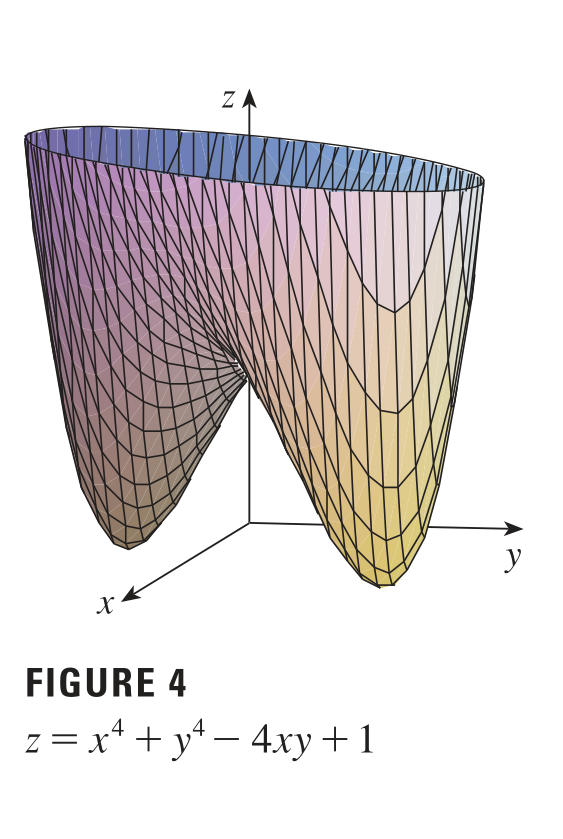
\includegraphics[width = 4.3 cm]{./images/min4.png}
  
\end{minipage}
\begin{minipage}[]{0.67\linewidth}
{\fontfamily{lmtt}\selectfont \textbf{\textcolor{blue5}{\faIcon{map-marker-alt} EXAMPLE.}}} Find the local maximum and minimum ad saddle points of $f(x,y) = x^4 + y^4 - 4xy + 1$.

First we have 
\begin{align*}
  f_x = 4x^3 - 4y & \quad & f_y = 4y^3 - 4x \\
  x^3 - y = 0 & \quad & y^3 - x = 0 
\end{align*}
which implies $0 = x^9 - x = x(x^2 - 1)(x^2 + 1)(x^4  + 1 )$, so there're 3 roots: 0, 1, -1. The 3 critical points are $(0,0), (1,1), (-1, -1)$.

Next we calculate the second partial derivatives and $D(x,y)$
\begin{align*}
  f_{xx} = 12x^2 & \quad & f_{xy} = -4 & \quad & f_yy = 12y^2 
\end{align*}
\[D(x,y) = f_{xx}f_{yy} - (f_{xy})^2 = 144 x^2 y^2 - 16 \]
Since $D(0,0) = -16 < 0$, it follows that (0,0) is a saddle point. And $D(1,1) = 128 >0, f_{xx}(1,1) = 12 > 0$, so it's a local minimum. Similarly, $(-1,-1)$ is a local minimum.
  
\end{minipage}\\
{\fontfamily{lmtt}\selectfont \textbf{\textcolor{blue5}{\faIcon{map-marker-alt} EXAMPLE.}}} Find the shortest distance from $(1,0,-2)$ to the plane $x + 2y + z = 4 $.

The distance from $(x,y,z )$ to $(1,0,-2 )$ is 
\[d^2 = f(x,y) = (x - 1)^2 + y^2 + (6-x-2y)^2   \]
By solving the equation 
\begin{align*}
  f_x = 4x + 4y -  14 = 0 \\
  f_y = 4x + 10y - 24 = 0 
\end{align*}
we find that the only critical point is $\left( \frac{11 }{6 }, \frac{5 }{3 } \right)$. Since $f_{xx} = 4, f_{xy} = 4, f_{yy} = 10 , D(x,y) = f_{xx}f_{yy} - (f_{xy})^2 = 24 > 0 $, so $f$ has a local minimum at $\left( \frac{11 }{6 }, \frac{5 }{3 } \right)$. There must be a point on the given plane that is closest to (1,0,-2). We also find that $d = \frac{5 }{6 } \sqrt{6 }$.


\subsection*{{\fontfamily{lmss}\selectfont \textcolor{blue5}{\faIcon{anchor} \underline{Absolute Maximum and Minimum Values}}}}
\begin{Def}[Extreme Value Theorem]
  If $f$ is continuous on a closed, bounded set $D \in \mathbb{R}^2$  then $f$ attains an absolute maximum value $f(x_1, y_1)$ and an absolute minimum value $f(x_2, y_2)$. 
  To find it, \\
  \textbf{\textcolor{blue5}{\fontfamily{lmss}\selectfont 1.}} Find the values of $f$ at the critical points of $f$ in $D$.\\
\textbf{\textcolor{blue5}{\fontfamily{lmss}\selectfont 2.}}  Find the extreme values of $f$ on the boundary of $D$.\\
\textbf{\textcolor{blue5}{\fontfamily{lmss}\selectfont 3.}}  Determine the largest and smallest ones.
\end{Def}

{\fontfamily{lmtt}\selectfont \textbf{\textcolor{blue5}{\faIcon{map-marker-alt} EXAMPLE.}}} Find the absolute maximum and minimum of $f(x,y) = x^2 - 2xy + 2y $ on the rectangle $D = \{(x,y) | \text{ }0 \le x \le 3, 0 \le y \le 2\}$.\\
Since $f$ is a polynominal, it's continuous on $D$. First find the critical points
\[f_x = 2x - 2y = 0 \quad \text{ } \quad f_y = -2x + 2 = 0 \]
So the only critical point is (1,1), and $f(1,1) = 1 $.

Now we look at the values of $f$ on the boundary of $D$, which consists of the four line segments $L_1, L_2, L_3, L_4$.

\begin{center}
  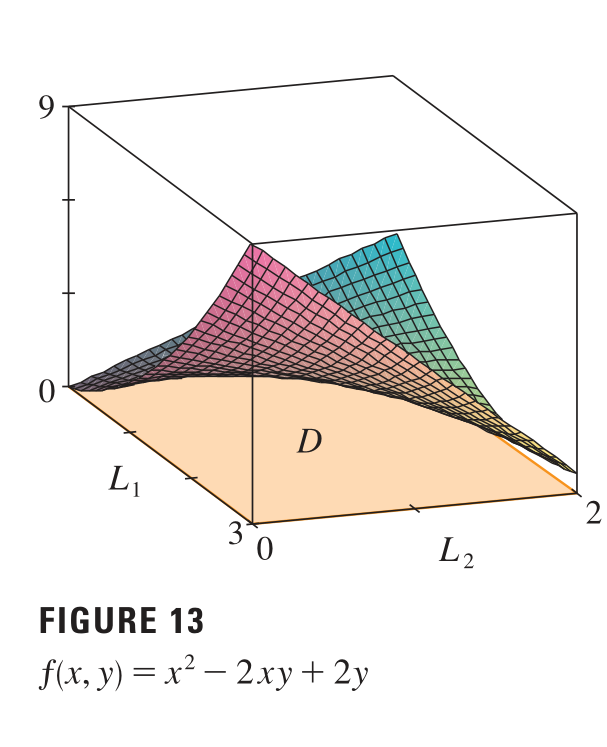
\includegraphics[width = 4.3 cm]{./images/fig13.png}
  
\end{center}

\begin{minipage}[]{0.3\linewidth}
  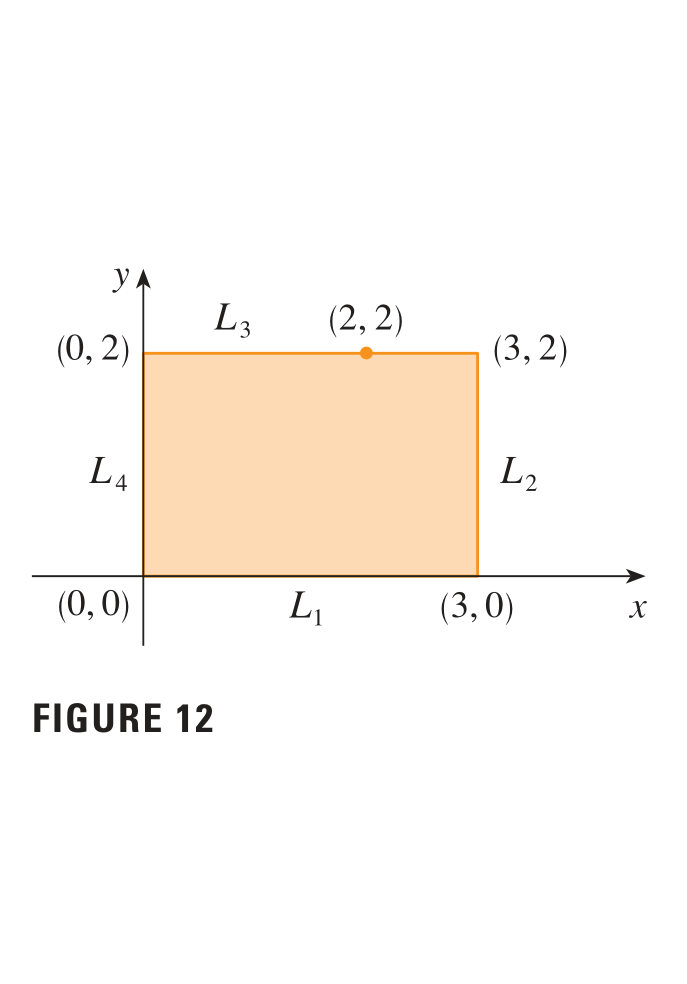
\includegraphics[width = 4.3 cm]{./images/rec12.png}
  
\end{minipage}
\begin{minipage}[]{0.67\linewidth}
 
\textcolor{blue5}{\small $\blacksquare$} On $L_1$, we have $y = 0 $ and 
\[f(x,0) = x^2 \quad \text{ } \quad 0 \le x \le 3 \]
Its minimum value is $f(0,0) = 0$ and maximum value is $f(3,0) = 9$.\\
\textcolor{blue5}{\small $\blacksquare$} On $L_2$, we have $x = 3$ and  
\[f(3, y) = 9  - 4y \quad \text{ } \quad 0 \le y \le 2   \]
The maximum value is $f(3,0) = 9 $ and the minimum value is $f(3,2) = 1$.\\
\textcolor{blue5}{\small $\blacksquare$} On $L_3$ we have $y = 2$ and 
\[f(x,2) = x^2 - 4x + 4 = (x- 2) ^2 \quad \text{ } \quad 0 \le x \le 3\]
The minimum value is $f(2,2) = 0$ and the maximum value is $f(0,2) = 4$.\\
\textcolor{blue5}{\small $\blacksquare$} On $L_4$ we have $x = 0$ and 
\[f(0,y) = 2y \quad \text{ } \quad 0 \le y \le 2 \]
with maximum value $f(0,2) = 4$ and minimum valye $f(0,0) = 0$.

Thus, on the boundary, the minimum value is 0 and the maximum is 9.

\end{minipage}

\begin{minipage}[]{0.3\linewidth}
  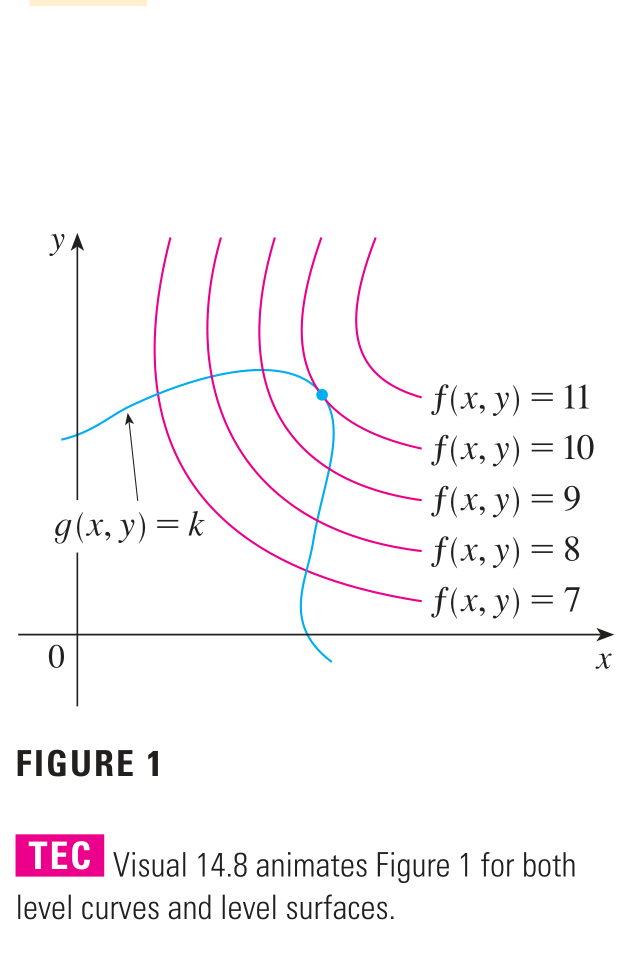
\includegraphics[width = 4.3 cm]{./images/lagrange.png}
  
\end{minipage}
\begin{minipage}[]{0.67\linewidth}
\subsection*{{\fontfamily{lmss}\selectfont \textcolor{blue5}{\faIcon{anchor} \underline{Lagrange Multipliers}}}}
We will discover Lagrange's methods for maximizing or minimizing a general function $f(x,y,z)$ to a constraint (or side contidition) of the form $g(x,y,z) = k$.
\end{minipage}

\begin{Def}[Method of Lagrange Multipliers]
  To find the maximum and minimum values of $f(x,y,z)$ to the constraint $g(x,y,z) = k$ (assume they exist and $\nabla g \ne \textbf{0}$ on the surface $g(x,y,z) = k$):\\
  (a) Find all $x,y,z$ and $\lambda $ (\textbf{Lagrange multiplier}) such that 
  \begin{align*}
    \nabla f(x,y,z) & = \lambda \nabla g(x,y,z) \\
    g(x,y,z) & = k 
  \end{align*}
  (b) Evaluate $f$ at all these points and find the largest and smallest ones.
\end{Def}  
Write (a) in terms of components 
\[f_x = \lambda g_x \quad \text{ } \quad f_y = \lambda g_y \quad \text{ } \quad f_z = \lambda g_z \quad \text{ } \quad g(x,y,z) = k\]
It's not necessary to find explicit values for $\lambda $.\\
{\fontfamily{lmtt}\selectfont \textbf{\textcolor{blue5}{\faIcon{map-marker-alt} EXAMPLE.}}} A rectangular box without a lid is to be made from 12 m$^2$ of cardboard. Find the maximum volume.

{\fontfamily{lmtt}\selectfont \textbf{\textcolor{blue5}{SOLUTION.}}}  We wish to maximize $V = xyz$, where $x,y,z$ are the length, width and height of the box, subject to the constraint 
\[g(x,y,z) = 2xz + 2yz + xy = 12\]
We look for $x,y,z, \lambda $ that $\nabla V = \lambda \nabla g$ and $g(x,y,z) = 12$. 
\begin{align*}
  V_x = \lambda g_x \\
  V_y = \lambda g_y \\ 
  V_z = \lambda g_z \\
  2xz + 2yz + xy = 12 
\end{align*}
which become 
\begin{align*}
  yz = \lambda (2z + y) \\
  xz = \lambda (2z + x) \\
  xy = \lambda (2x + 2y) \\
  2xz + 2yz + xy = 12 
\end{align*}
Observe that $\lambda \ne 0$, and we have $2xz + xy = 2yz + xy$ which gives $xz = yz$. But $z \ne 0 $, or $V = 0 $. So $x = y$. We also have $x = y = 2z$.
\[4 z^2 + 4 z^2 + 4 z^2 = 12 \]
Therefore we have $x = y =2$, and $z = 1$.

\begin{minipage}[]{0.3\linewidth}
  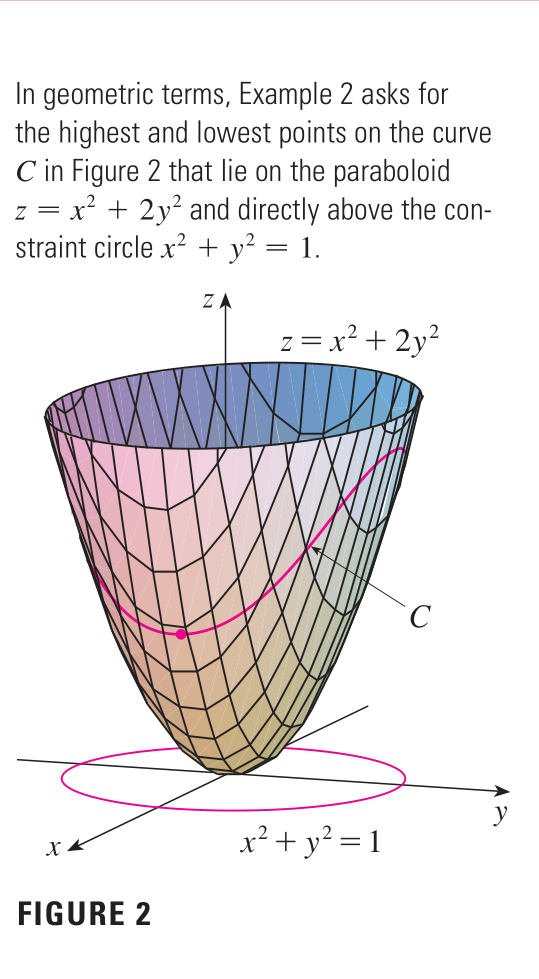
\includegraphics[width = 4.3 cm]{./images/lagrange2.png}\\
  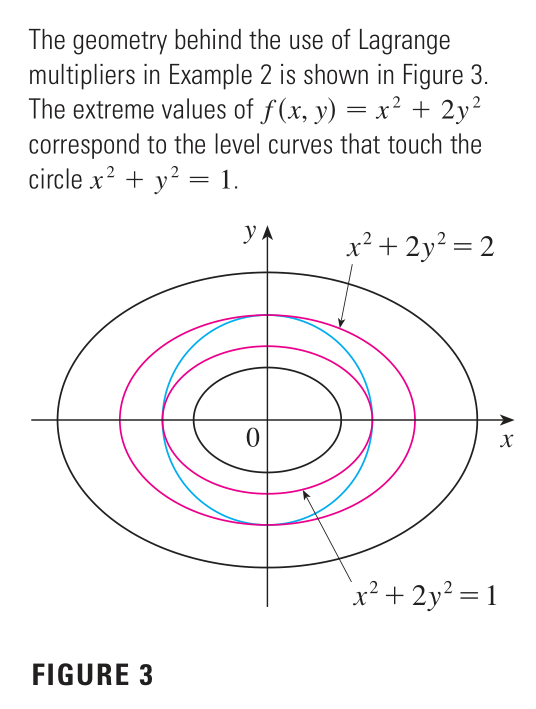
\includegraphics[width = 4.3 cm]{./images/lagrange3.png}
  
  
\end{minipage}
\begin{minipage}[]{0.67\linewidth}
  {\fontfamily{lmtt}\selectfont \textbf{\textcolor{blue5}{\faIcon{map-marker-alt} EXAMPLE.}}} Find the extreme values of $f(x,y) = x^2 + 2 y^2 $ on the circle $x^2 + y^2 = 1 $.  

  Solve the equation 
  \begin{align*}
  f_x = \lambda g_x, \quad & f_y = \lambda g_y, \quad g(x,y) = 1\\
   &  2x = 2x \lambda \\
   &  4y = 2y \lambda \\
   &  x^2 + y^2 = 1 
  \end{align*}
\textcolor{blue5}{\small $\blacksquare$} $x = 0$, then $y = \pm 1$.\\
\textcolor{blue5}{\small $\blacksquare$} $\lambda = 1$, then $y = 0$, and $x = \pm 1$.\\
Evaluating $f$ at these 4 points, we find that $f_ \text{max} = f(0, \pm 1) = 2$ and $f_ \text{min} = f(\pm 1, 0) = 1 $.
\end{minipage}

{\fontfamily{lmtt}\selectfont \textbf{\textcolor{blue5}{\faIcon{map-marker-alt} EXAMPLE.}}} Find the points on the sphere $x^2 + y^2 + z^2 = 4 $ that are closest and farthest from $(3,1,-1)$.

\begin{minipage}[]{0.34\linewidth}
  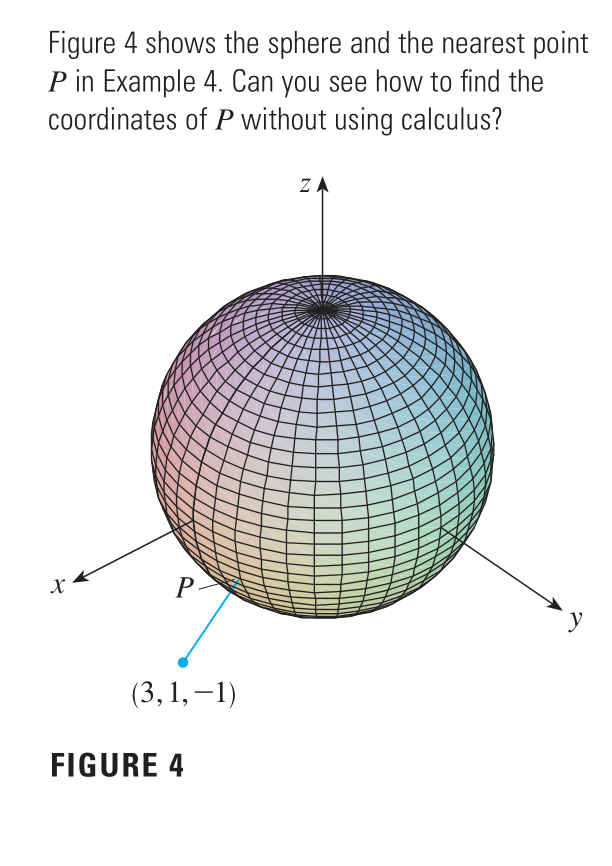
\includegraphics[width = 5 cm]{./images/lagrange4.png}
  
\end{minipage}
\begin{minipage}[]{0.63\linewidth}
{\fontfamily{lmtt}\selectfont \textbf{\textcolor{blue5}{SOLUTION.}}} We want to minimize and maximize 
\[d^2 = (x-3)^2 + (y-1)^2 + (z + 1)^2 \]
The constraint is that the point $(x,y,z)$ lies on the sphere, that is 
\[g(x,y,z) = x^2 + y^2 + z^2 = 4  \]
According to the method of Lagrange multipliers, we solve $\nabla f = \lambda \nabla g, g = 4 $, which gives 
\begin{equation*}
  \begin{split}
    2(x- 3) = 2x \lambda \\ 
    2(y-1) = 2y \lambda \\
    2(z + 1) = 2z \lambda \\ 
    x^2 + y^2 + z^2 = 4     
  \end{split}
\end{equation*}
  
\end{minipage}

Hence, we got $x = \cfrac{3 }{1 - \lambda }, y = \cfrac{1 }{1 - \lambda }, z = - \cfrac{1 }{ 1 - \lambda }   $. Then we have 
\[ \cfrac{3^2 }{(1- \lambda )^2} + \cfrac{1^2 }{(1 - \lambda )^2 } + \cfrac{(-1)^2 }{(1 - \lambda )^2} = 4\]
which gives $\lambda = 1 \pm \cfrac{\sqrt{11 }}{2 }$, which give the corresponding $(x,y,z)$ 
\[\left( \cfrac{6 }{\sqrt{11}}, \cfrac{2 }{ \sqrt{11 }}, - \cfrac{2 }{\sqrt{11 }} \right) \quad \text{and} \quad \left( - \cfrac{6 }{\sqrt{11 }}, - \cfrac{2 }{\sqrt{11 }}, \cfrac{2 }{\sqrt{11 }} \right)\]
which is the closest and farthest point, respectively.

\subsection*{{\fontfamily{lmss}\selectfont \textcolor{blue5}{\faIcon{anchor} \underline{Two Constraints}}}}
We want to find the maximum and minimum values of $f(x,y,z)$ subject to 2 constraints of the form $g(x,y,z) = k $ and $g(x,y,z) = c $. Geometrically, we are looking for the extreme values of $f$ when $(x,y,z)$ lies on the curve of intersection $C$ of $g$ and $h$. 
\begin{mdframed}
  \[\nabla f(x_0, y_0, z_0) = \lambda \nabla g(x_0, y_0, z_0) + \mu \nabla h (x_0, y_0, z_0 )\]
\end{mdframed}
Solving 5 equations 
\begin{equation*}
  \begin{split}
    f_x  = \lambda g_x + \mu h_x \\
    f_y  = \lambda g_y + \mu h_y \\
    f_z  = \lambda g_z + \mu h_z \\
    g(x,y,z) = k \\
    h(x,y,z) = c
  \end{split}
\end{equation*}
{\fontfamily{lmtt}\selectfont \textbf{\textcolor{blue5}{\faIcon{map-marker-alt} EXAMPLE.}}} Find the maximum value of $f(x,y,z) = x + 2y + 3z$ on the curve of intersection  of the plane $x - y + z = 1 $ and the cylinder $x^2 + y^2 = 1 $.

\begin{minipage}[]{0.3\linewidth}
  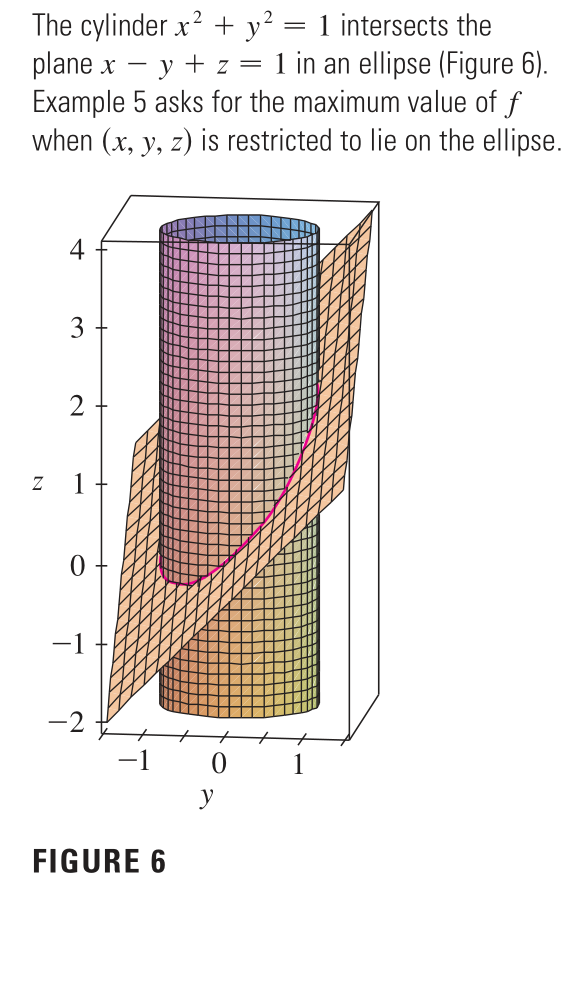
\includegraphics[width = 4.3 cm]{./images/2constraints.png}
  
\end{minipage}
\begin{minipage}[]{0.67\linewidth}
{\fontfamily{lmtt}\selectfont \textbf{\textcolor{blue5}{SOLUTION.}}} 
We maximize $f(x,y,z) = x + 2y + 3z $. We solve the equations 
\begin{equation*}
  \begin{split}
    1 & = \lambda + 2x \mu \\
    2 & = - \lambda + 2y \mu \\ 
    3 &  = \lambda \\
    x & - y + z = 1 \\
    x^2 &  + y^2 = 1 
  \end{split}
\end{equation*}
We get $x = -1/\mu , y = 5 / (2 \mu  )$. 
\[\cfrac{1 }{\mu ^2 } + \cfrac{25 }{4 \mu ^2 } = 1 \]
and so $\mu = \pm \frac{\sqrt{29} }{2 }$  . Then $x = \mp 2/ \sqrt{29 }, y = \pm 5 / \sqrt{29 }, z = 1 \pm 7/ \sqrt{29 }  $. The corresponding values of $f $ are $3 \pm \sqrt{29 }$. The maximum value of $f$ on the given curve is $3 + \sqrt{29 }$.
  
\end{minipage}

Suppose we let $x$ vary while keeping $y$ fixed ($y = b$) in $f(x,y)$, we got a function $g(x) = f(x,b)$. If $g$ has a derivative at $a$, we call it the \textbf{partial derivative of \textit{f} with respect to \textit{x} at \textit{(a,b)}}. We have 
\[g'(a) = \lim_{h \to  0 }\frac{g(a + h) - g(a)}{h }\]
and so it become $\quad$
\begin{minipage}[]{0.6\linewidth}
\begin{mdframed}
\[f_x (x,y) = \lim_{h \to 0} \frac{f(x + h, b) - f(x,y)}{h }\]
\[f_y (x,y) = \lim_{h \to 0} \frac{f(x , y + h) - f(x,y)}{h }\]
  \end{mdframed}
\end{minipage}

To compute partial derivatives, we have the following rule.
\begin{mdframed}
  {\fontfamily{lmtt}\selectfont \textbf{\textcolor{blue5}{\small $\blacksquare$ Rule for Finding Partial Derivatives of $z = f(x,y)$}}} \\
{\fontfamily{lmtt}\selectfont \textbf{\small 1.}} To find $f_x$, regard $y$ as a constant and differentiate $f(x,y)$ with respect to $x$.\\
{\fontfamily{lmtt}\selectfont \textbf{\small 2.}} To find $f_y$, regard $x$ as a constant and differentiate $f(x,y)$ with respect to $y$.
\end{mdframed}
{\fontfamily{lmtt}\selectfont \textbf{\textcolor{blue5}{{\small \faIcon{map-marker-alt}} EXAMPLE.}}} If $f(x,y) = x^3 + x^2 y^3 - 2y^2$, find $f_x(2,1)$ and $f_y(2,1)$.
Holding $y$ constant and differentiating with respect to $x$, we get 
\begin{equation*}
  \begin{split}
 &   f_x(x,y) = 3 x^2 + 2x y^3 \\
 &  f_x(2,1) = 3 \cdot 2^2 + 2 \cdot 2 \cdot 1^3 = 16
  \end{split}
\end{equation*}
Do the same with $y$
\begin{equation*}
  \begin{split}
    & f_y (x,y) = 3 x^2 y^2 - 4y \\
    & f_y (2,1) = 3 \cdot 2^2 \cdot 1^2 - 4 \cdot 1 = 8       
  \end{split}
\end{equation*}

\subsection*{{\fontfamily{lmss}\selectfont \underline{Interpretations of Partial Derivatives}}}

\begin{minipage}[]{0.34\linewidth}
  \begin{center}
    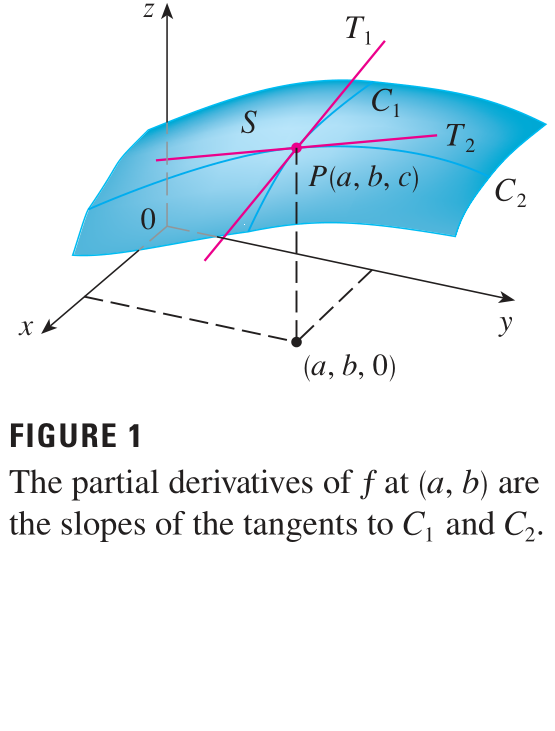
\includegraphics[width = 4.3 cm]{./images/interpretation.png} 
  \end{center}
\end{minipage}
\begin{minipage}[]{0.6\linewidth}
\textcolor{blue5}{\small $\blacksquare$}  The equation $f(x,y)$ represent a surface $S$. By fixing $y = b$, we got the curve $C_1$ (the trace of $S$ in the pane $y = b $).

\textcolor{blue5}{\small $\blacksquare$}  Notice that $C_1 $ is the graph of $g(x) = f(x, b )$, so the slope of its tangent $T_1$ is $g'(a) = f_x(a,b)$.
\end{minipage}

\begin{minipage}[]{0.34\linewidth}
  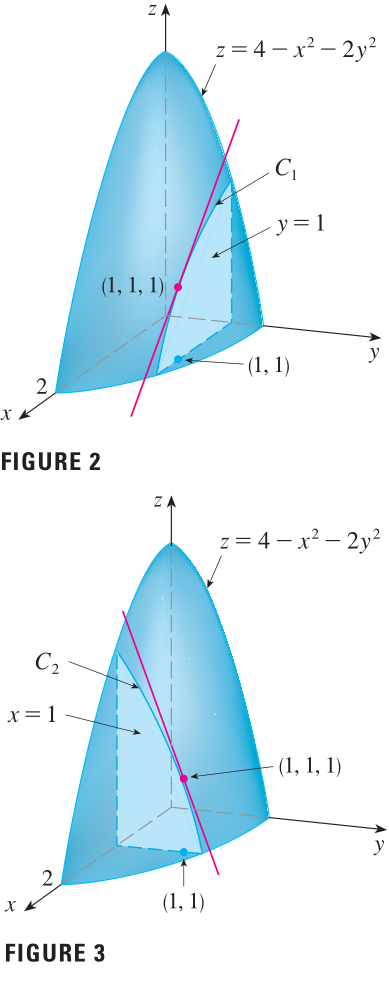
\includegraphics[width = 4  cm]{./images/pareg2.png}
  
\end{minipage}
\begin{minipage}[b]{0.63\linewidth}

 {\fontfamily{lmtt}\selectfont \textbf{\textcolor{blue5}{{\small \faIcon{map-marker-alt}} EXAMPLE.}}} If $f(x,y) = x^3 + x^2 y^3 - 2 y^2 $, find $f_x (1,1)$ and $f_y (1,1)$ and interpret these numbers as slopes.

 We have 
 \begin{equation*}
   \begin{split}
      f_x (x,y) = -2x & \quad \text{ } \quad f_y (x.y) = -4y \\
      f_x(1,1) = -2 & \quad  \text{ } \quad f_y(1,1) = -4  
   \end{split}
 \end{equation*}
 
 The vertical plane $y = 1 $ intersects $f(x,y)$ in the parabola $z = 2 - x^2 $, $y = 1$ ($C_1$). The slope of the tangent line to this parabola at the point $(1,1,1)$ is $f_x (1,1) = -2 $.
\end{minipage}\\
{\fontfamily{lmtt}\selectfont \textbf{\textcolor{blue5}{{\small \faIcon{map-marker-alt}} EXAMPLE.}}} If $f(x,y) = \sin{\left(\cfrac{x }{1 + y }\right)}$, calculate $\cfrac{\delta f }{\partial x }$ and $\cfrac{\delta f}{\partial y}$.

\textcolor{blue5}{\small $ \blacksquare$} Using the Chain Rule for functions of one variable, we have 
\begin{equation*}
  \begin{split}
    & \frac{\partial f }{\partial x } = \cos{\left( \frac{x }{ 1 + y }  \right)} \cdot \frac{\partial}{\partial x } \left( \frac{x }{1 + y }  \right) = \cos{ \left( \frac{x }{1 + y }\right)} \cdot \frac{1 }{1 + y } \\ 
    & \frac{\delta f }{\partial y } = \cos{\left( \frac{x }{ 1 + y }  \right)} \cdot \frac{\partial }{\partial y } \left( \frac{x }{1 + y }  \right) = -  \cos{ \left( \frac{x }{1 + y }\right)} \cdot \frac{x }{(1 + y)^2 } 
  \end{split}
\end{equation*}
{\fontfamily{lmtt}\selectfont \textbf{\textcolor{blue5}{{\small \faIcon{map-marker-alt}} EXAMPLE.}}} Find $\partial z / \partial x $ and $ \partial z / \partial y $ of $z $ is defined as follow 
\[x ^ 3 + y ^ 3 + z ^ 3 + 6 xyz = 1 \]


\begin{minipage}[b]{0.28\linewidth}
  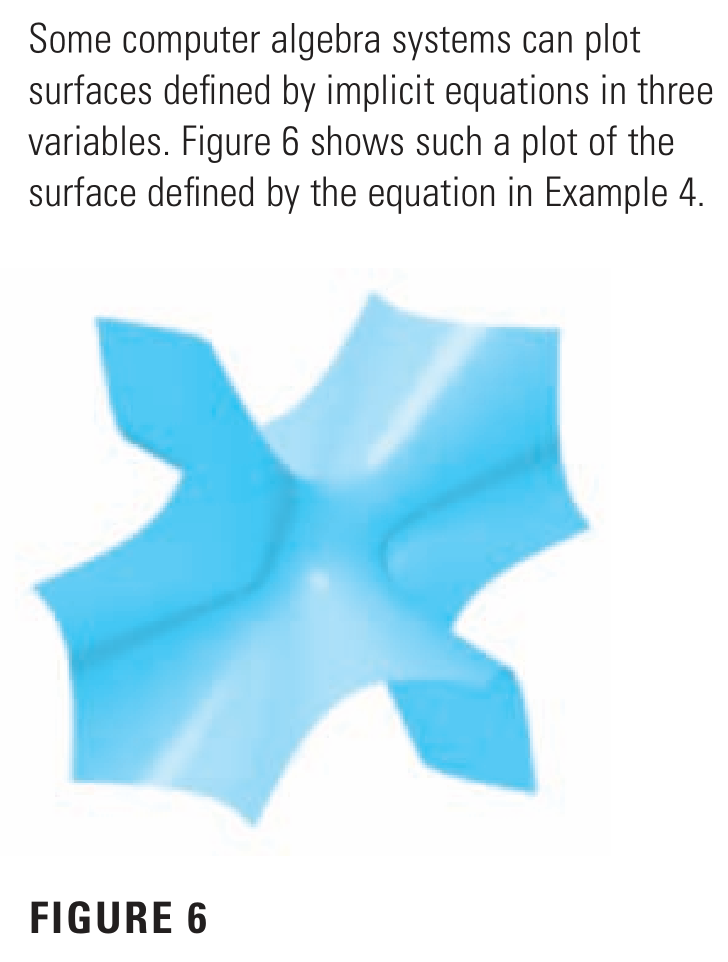
\includegraphics[width = 4.3 cm]{./images/partialeg4.png}
  \end{minipage}
\begin{minipage}[b]{0.67\linewidth}
\textcolor{blue9}{\small $\blacksquare$} First differentiate implicitly with respect to $x $, treat $y $ as a constant.
\[3 x^2 + 3 z^2 \frac{\partial z }{ \partial x } + 6yz + 6xy \frac{\partial z }{ \partial x }= 0\]
Solving this for $\partial z / \partial x $, we obtain 
\[ \frac{\partial z }{\partial x } = - \frac{y^2 + 2xz }{z^2 + 2xy }\]
Similarly, implicit differentiation with respect to $y $ gives 
\[\frac{\partial z }{\partial y } = - \frac{y^2 + 2xz }{z^2 + 2xy }\]
\end{minipage}

\subsection*{{\fontfamily{lmss}\selectfont \underline{Functions of More Than Two Variables }}}  
Regarding $y$ and $z$ as constants and differentiating with respect to $x$.
\[f_x (x, y, z) = \lim_{h \to 0 } \frac{f(x + h, y, z) - f(x,y,z)}{h }\]
{\fontfamily{lmtt}\selectfont \textbf{\textcolor{blue5}{{\small \faIcon{map-marker-alt}} EXAMPLE.}}}  Find $f_x, f _ y $, and $f _ z $ if $f(x,y,z) = e^{xy} \ln{z}$.

Holding $y$ and $z $ constant and differentiating with respect to $x $, we have 
\[f_x = y e^{xy} \ln{z}\]

Similarly, \[f_y = x e^{xy} \ln {z} \quad  \text{and} \quad f_z = \cfrac{e^{xy}}{z }\]

\subsection*{{\fontfamily{lmss}\selectfont \underline{Higher Derivatives}}}

If $f$ is a function of 2 variables, then $f_x$ and $f _ y $ are also functions of 2 variables.  So we can consider the \textbf{second partial derivatives} of $f$, that is $(f_x)_x$, $(f_x)_y $, $(f_y)_x $, and $(f_y)_y $.
\begin{equation*}
  \begin{split}
    & (f _ x ) _ x = f _ {xx} = f _ {11} = \frac{\partial }{\partial x } \left( \frac{\partial f }{ \partial x }\right) = \frac{\partial ^2 f }{\partial  x^2 } = \frac{\partial ^2 z }{\partial x^2 } \\
    & (f _ x ) _ y = f _ {xy} = f _ {12} = \frac{\partial }{\partial y } \left( \frac{\partial f }{ \partial x }\right) = \frac{\partial ^2 f }{\partial  y \text{ } \partial x } = \frac{\partial ^2 z }{\partial y \text{ }\partial x } \\
    & (f _ y ) _ x = f _ {yx} = f _ {21} = \frac{\partial }{\partial x } \left( \frac{\partial f }{ \partial y }\right) = \frac{\partial ^2 f }{\partial  x \text{ } \partial y } = \frac{\partial ^2 z }{\partial x \text{ }\partial y } \\
& (f _ y ) _ y = f _ {yy} = f _ {22} = \frac{\partial }{\partial y } \left( \frac{\partial f }{ \partial y }\right) = \frac{\partial ^2 f }{\partial  y^2 } = \frac{\partial ^2 z }{\partial y^2 }
  \end{split}
\end{equation*}
Thus $f_{xy}$ (or $\partial ^2 f / \partial y \text{ } \partial x $) means that we first differentiate with respect to $x $ and then with respect to $y $.\\
{\fontfamily{lmtt}\selectfont \textbf{\textcolor{blue5}{{\small \faIcon{map-marker-alt}} EXAMPLE.}}} Find the second partial derivatives of 
\[f(x,y) = x ^ 3 + x^2 y^3 - 2 y^2 \]
{\fontfamily{lmss}\selectfont \textcolor{blue5}{\small SOLUTION}} We find that 
\[f_x(x,y) = 3 x^2 + 2x y^3 \quad \text{ } \quad f_y(x,y) = 3 x^2 y^2 - 4y \]
Therefore 
\begin{equation*}
  \begin{split}
    f _ {xx} = \frac{\partial }{\partial x } (3 x^2 + 2xy^3)  = 6x + 2 y^3 & \quad \text{ }  \quad f _ {xy} = \frac{\partial }{ \partial y } (3 x^2 + 2 x y^3) = 6x y^2 \\
    f _ {yx} = \frac{\partial }{\partial x } (3 x^2 y^2 - 4y) = 6x y^2 & \quad \text{ } \quad f_{yy} = \frac{\partial }{\partial y } (3 x^2 y^2 - 4y ) = 6 x^2 y - 4 
  \end{split}
\end{equation*}
\begin{mdframed}
  \textbf{\textcolor{pink}{\fontfamily{lmss}\selectfont Clairaut's Theorem}} $\quad$ Suppose $f $ is defined on a disk $D $ that contains the point $(a, b )$. If the functions $f _ {xy}$ and $f _ {yx }$ are both continuous in $D $, then 
  \[f _ {xy} (a, b) = f _ {yx} (a, b )\]
\end{mdframed}
Partial derivatives of order 3 or higher can also be defined
\[f _ {xyy} = (f _ {xy}) _ y = \frac{\partial }{ \partial y } \left( \frac{\partial ^2 f }{\partial x \text{ } \partial y }\right) = \frac{\partial ^3 f }{\partial y^2 \text{ } \partial x}\]
and using Clairaut's Theorem it can be shown that $f _ {xyy} = f _ {y xy} = f _ {yy x }$. \\
{\fontfamily{lmtt}\selectfont \textbf{\textcolor{blue5}{{\small \faIcon{map-marker-alt}} EXAMPLE.}}} Calculate $f _ {xxyz}$ if $f(x,y,z) = \sin{3x + yz}$. \\
\textbf{\textcolor{blue5}{\fontfamily{lmss}\selectfont \small SOLUTION.}} $\quad $ 
\begin{equation*}
  \begin{split}
     f _ {x} & = 3 \cos{(3x + yz) } \\
     f _ {xx} & = -9 \sin{(3x + yz)} \\
     f _ {xxy} & = -9z \cos{(3x + yz)} \\
     f _ {xxyz} & = -9 \cos{(3x + yz)} + 9yz \sin{(3x + yz)}
  \end{split}
\end{equation*}

\subsection*{{\fontfamily{lmss}\selectfont \underline{Partial Differential Equations}}}
\textbf{Laplace's equation.}
$$\cfrac{\partial ^2 u }{\partial x^2 } + \cfrac{\partial ^2 u }{\partial y^2 } = 0 $$

\section{Tangent Planes and Linear Approximations}
As we zoom in toward a point on a surface of a differentiable function, the surface looks more and more like a plane (its tangent plane) and we can approximate it by a linear function of 2 variables.

\begin{minipage}[b]{0.34\linewidth}
  \begin{center}
    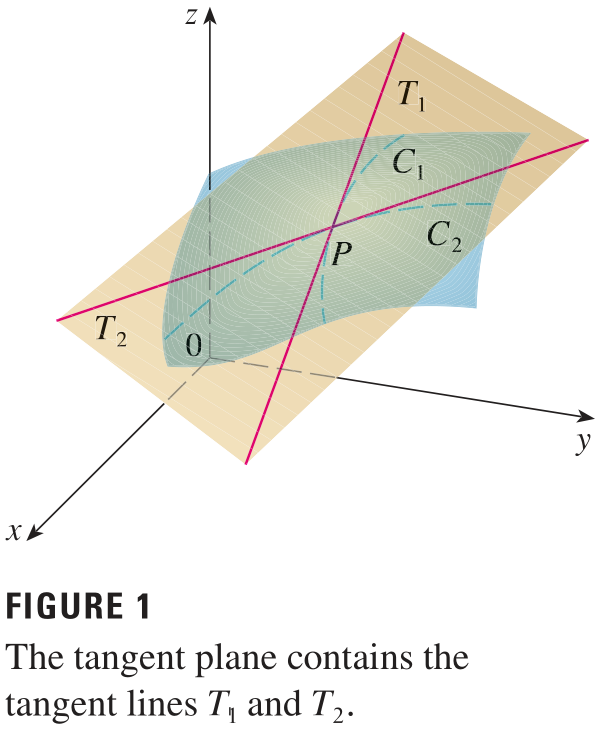
\includegraphics[width = 4.3 cm]{./images/tangentplane.png} 
  \end{center}
  
\end{minipage}
\begin{minipage}[b]{0.63\linewidth}
  \subsection*{{\fontfamily{lmss}\selectfont \underline{Tangent Planes}}}
  Suppose surface $S$ of $z = f(x,y)$ has continuous first partial derivatives, let $P(x _ 0,  y _ 0, z _ 0 ) \in S$. \\
  \textcolor{blue5}{$\blacksquare$} $C _ 1 $ and $C _ 2 $ be the curves obtained by intersecting the vertical planes $y = y _ 0 $ and $ x = x0 $ with $S $.\\
 \textcolor{blue5}{$\blacksquare$} Let $T _ 1 $  and $T _ 2 $ be the tangent lines to the curves  $C _ 1 $ and $ C _ 2$ at $P$. 
 Then the \textbf{tangent plane} to the surface $S $ at the point $P $ contains $T _ 1 $ and $T _ 2 $. In fact, it consists of \textit{all possible} tangent lines at $P $.\\
\textcolor{blue5}{$\blacksquare$} We know the plane has an equation of the form 
\[A(x - x _ 0) + B(y - y _ 0) + C(z - z _ 0 ) = 0 \]
By dividing this by $C $ and letting $a = -A/C $ and $b = -B/C $, 
\[z - z _ 0 =  a(x - x _ 0 ) + b (y - y _ 0 )\]
\end{minipage}

The tangent plane's intersection with the plane $y = y _ 0 $ must be the tangent line $T _ 1 $.
\[z - z _ 0 = a(x - x _ 0 ) \quad \text{ where } y = y _ 0\]

This is a line with slope $a = f _ x (x _ 0, y _ 0  )$. Similarly, $z - z _ 0 = b ( y - y _ 0 )$, and $b = f _ y (x _ 0, y _ 0 )$.

\begin{Def}[Equation of Tangent Plane]
  Suppose $f $ has continuous partial derivatives. An equation of the tangent plane to the surface $z = f(x,y) $ at the point $P(x _ 0, y _ 0, z  _ 0 )$ is 
  \[z - z _ 0 = f_x(x _ 0, y _ 0) (x - x _ 0) + f_y (x _ 0, y _ 0) (y - y _ 0 )\]
\end{Def}
{\fontfamily{lmtt}\selectfont \textbf{\textcolor{blue5}{{\small \faIcon{map-marker-alt}} EXAMPLE.}}} Find the tangent plane to the elliptic paraboloid $z = 2 x^2  + y^2 $ at the point (1, 1, 3).
\begin{align*}
  &f_x(x,y) = 4x & & f_y(x,y) = 2y \\ 
  &f_x(1,1) = 4 & & f_y(1,1) = 2 
\end{align*}    
Then the equation of the tangent plane at (1, 1, 3) is 
\begin{equation*}
  \begin{split}
    z - 3 & = 4(x-1) + 2(y - 1) \\
    z & = 4x + 2y - 3 
  \end{split}
\end{equation*}
\begin{center}
  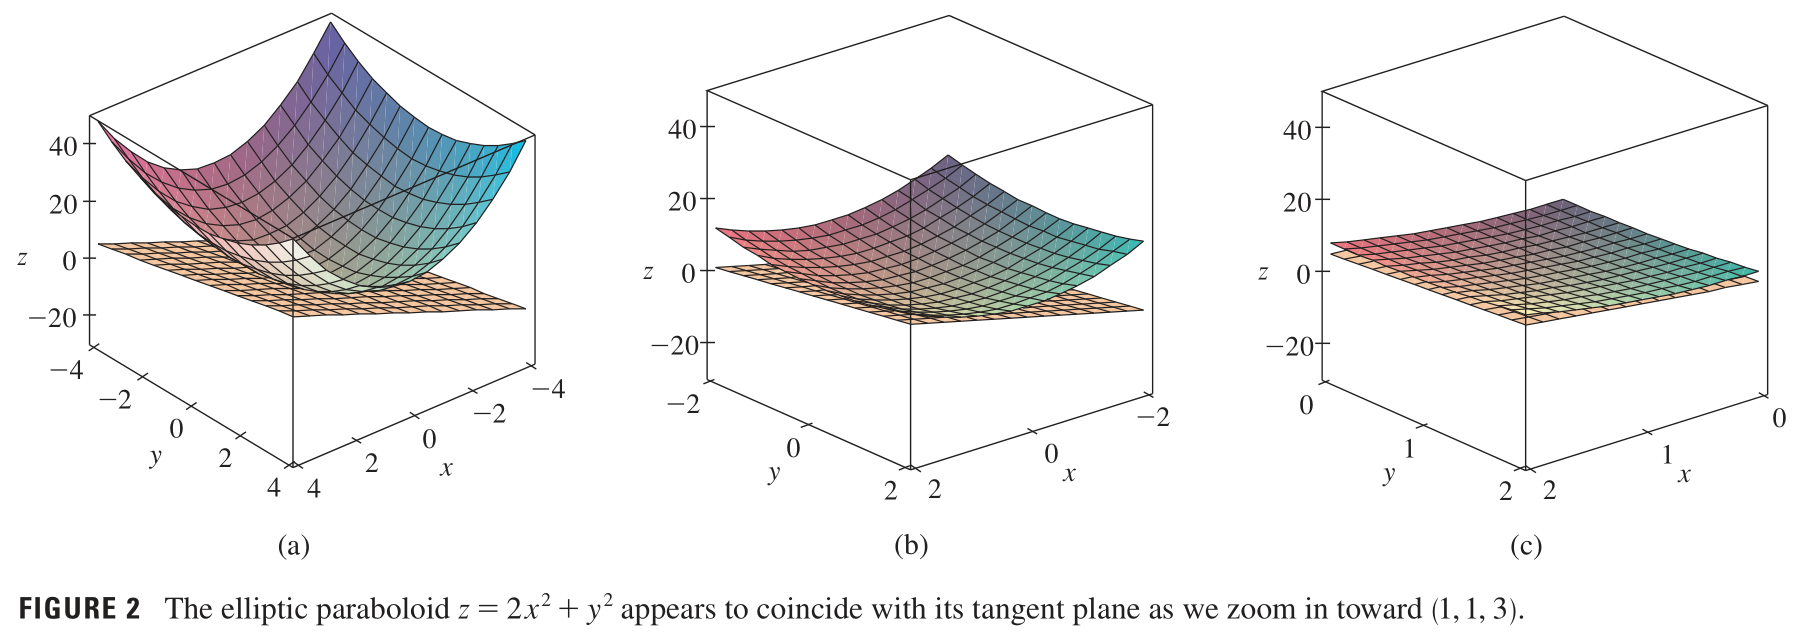
\includegraphics[width = 16 cm]{./images/tangent1.png} 
\end{center}

\begin{minipage}[]{0.34\linewidth}
\hfill  
\end{minipage}
\begin{minipage}[]{0.63\linewidth}
  By zooming toward the point $(1, 1)$ on a contour map, we see that the more we zoom in, the more the level curves look like equally spaced parallel lines.
\end{minipage}

\begin{center}
  \includegraphics[width = 16 cm]{./images/tangent2.png } 
\end{center}

\begin{minipage}[]{0.54\linewidth}
\subsection*{{\fontfamily{lmss}\selectfont \underline{Linear Approximations}}}
The equation of the tangent plane of $f(x,y) = 2 x^2 + y^2 $ at the point (1, 1, 3) is $z = 4x + 2y - 3 $. Therefore, the linear function of 2 variables 
\[L(x,y) = 4x + 2y - 3 \]
is the \textit{linearization of f} at (1, 1) and the approximation 
\[f(x,y) \approx 4x + 2y - 3 \]
is the \textit{linear approximation} or \textit{tangent plane approximation} of $f$ at (1, 1).
\end{minipage} \hfill
\begin{minipage}[]{0.42\linewidth}
  \begin{mdframed}
Eg: At the point $(1.1,0.95)$, the linear approximation gives 
\[f(1.1,0.95) \approx 4(1.1) + 2(0.95) - 3 = 3.3\]
True value: $f(1.1, 0.95) = 2(1.1)^2 + (0.95)^2 = 3.3225$.
  \end{mdframed}
\end{minipage}

\begin{Def}[]
\textbf{\textcolor{blue5}{\fontfamily{lmss}\selectfont The linearization of $f$ at $(a,b)$.}} $L(x,y) = f(a,b) + f _ x (a,b) (x-a) + f _ y (a,b)(y-b)$\\
\textbf{\textcolor{blue5}{\fontfamily{lmss}\selectfont The linear approximation of $f$ at $(a,b)$.}} $f(x,y) \approx f(a,b) + f _ x (a,b) (x-a) + f _ y (a,b)(y-b)$
\end{Def}

\begin{minipage}[]{0.34\linewidth}
  \begin{center}
    \includegraphics[width = 4.3 cm]{./images/linear.png}
    
  \end{center}
  
\end{minipage}
\begin{minipage}[]{0.63\linewidth}
What if $f _ x $ and $ f _ y $ are not continuous? 
\[f(x,y) = \begin{cases}
  \cfrac{xy }{x^2 + y^2 }& \text{ if } (x,y) \ne (0,0) \\
  0 & \text{ if } (x,y) = (0,0)
\end{cases}\]
Even though $f_x (0,0) = f_y (0,0) = 0$, but they are not continuous.
The linear approximation would be $f(x,y) \approx 0 $, but $f(x,y) = \frac{1 }{2 }$ at all points on the line $y = x $. So we define it as follow.
\end{minipage}

\begin{Def}[Differentiable]
  If $z = f(x,y)$, then $f $ is \textbf{differentiable} at $(a,b)$ if $\Delta z $ can be expressed as 
  \[\Delta z = f_x (a,b) \Delta x + f_y(a,b) \Delta y + \varepsilon _1 \Delta x + \varepsilon _2 \Delta y \]
  where $\varepsilon _ 1 $ and $ \varepsilon _ 2 \to 0$ as $(\Delta x, \Delta y) \to (0,0)$ .
\end{Def}
\pagebreak
Pretty ..dumb.
\begin{mdframed}
  \textbf{\textcolor{blue5}{\fontfamily{lmss}\selectfont Theorem.}} If $f_x$ and $f_y $ exist near $(a,b)$ and are continuous at $(a,b)$, then $f $ is differentiable at $(a,b)$.
\end{mdframed}
\begin{minipage}[]{0.28\linewidth}
  \includegraphics[width = 4.3 cm]{./images/leg2.png}
  
\end{minipage}\hfill
\begin{minipage}[]{0.69\linewidth}
  {\fontfamily{lmtt}\selectfont \textbf{\textcolor{blue5}{{\small \faIcon{map-marker-alt}} EXAMPLE.}}} Show that $f(x,y) = xe^{xy}$ is differentiable at  (1,0) and find its linearization there. Approximate f(1.1, -0.1).

  The partial derivatives are 
  \begin{align*}
    & f_x(x,y) = e^{xy} + x y e^{xy} & & f_x(x,y) = x^2 e^{xy} \\
    & f_x(1,0)  = 1 & & f_y(1,0) = 1
  \end{align*}  
  Both $f_x$ and $f_y $ are continuous, so by the above Theorem, we got $f$ differentiable. The linearization is 
  \begin{align*}
    L(x,y) & = f(1,0) + f_x (1,0)(x-1) + f _ y (1,0)(y - 0) \\
           & = x + y 
  \end{align*}
  So $f(1.1, -0,1) \approx 1.1 - 0.1 = 1 $, actual value: $0.98542 $.
\end{minipage}

\begin{minipage}[]{0.3\linewidth}
  \includegraphics[width = 4.3 cm]{./images/tangentline.png}
\end{minipage}
\begin{minipage}[b]{0.67\linewidth}
\subsection*{{\fontfamily{lmss}\selectfont \underline{\textcolor{blue5}{Differentials}}}}
\textcolor{blue5}{$\blacksquare$} For $y = f(x)$, we define $dx$ an independent variable. And $dy = f'(x)\,dx$, represents the change in height when $x$ changes $dx$. 

\textcolor{blue5}{$\blacksquare$} For a differentiable $z  = f(x,y )$, we define the \textbf{differentials} $dx $ and $dy $ to be independent variables.


\end{minipage}

\begin{Def}[Total differential]
  
Then the \textbf{differential} $dz$ (the \textbf{total differential}), is defined as follow.
  \[dz = f_x(x,y)\,dx + f_y(x,y)\,dy = \cfrac{\partial z }{\partial x }\, dx + \cfrac{\partial z }{ \partial y }\, dy \]
\end{Def}
If we take $dx = \Delta x = x - a $ and $dy = \Delta y = y - b $, then $f(x,y) \approx f(a,b) + dz $.

\begin{center}
  \includegraphics[width = 13 cm]{./images/tangentplaneapp.png} 
\end{center}

\begin{minipage}[]{0.3\linewidth}
  \includegraphics[width = 4.3 cm]{./images/fig8.png}
\end{minipage}
\begin{minipage}[]{0.64\linewidth}
  {\fontfamily{lmtt}\selectfont \textbf{\textcolor{blue5}{{\small \faIcon{map-marker-alt}} EXAMPLE.}}} \\
  (a) If $z = f(x,y) = x^2 + 3xy - y^2 $, find the differential $dz $.\\
  (b) If $x $ changes from 2 to 2.05 and $y $ changes from 3 to 2.96, comppare the values of $\Delta z $ and $dz$.

  \noindent
  {\fontfamily{lmtt}\selectfont \textbf{\textcolor{blue5}{SOLUTION}}} \\
  (a) Applying the formula, \[dz = \,dy = \cfrac{\partial z }{\partial x }\, dx + \cfrac{\partial z }{ \partial y }\, dy = (2x + 3y) \,dx + (3x - 2y)\,dy\]
  (b) Putting $x = 2, \,dx = \Delta x = 0.05, y = 3, dy = \Delta y = -0.04$, we get
  \[dz = [2(2) + 3 (3)]0.05 + [3(2) - 2(3)](-0.04) = 0.65\]
  The increment of $z $ is 
  \begin{align*}
    \Delta z & = f(2.05, 2.96) - f(2,3) \\
             & = [(2.05)^2 + 3(2.05)(2.96) - (2.96)^2] - [2^2 + 3(2)(3) - 3^2] \\
             &= 0.6449
  \end{align*}
{\small \faIcon{greater-than}}
Notice that $\Delta z \approx dz$ but $dz $ is easier to compute.

\end{minipage}

\subsection*{{\fontfamily{lmss}\selectfont \underline{Functions of Three or More Variables}}}
\textbf{Linear approximation.} $f(x,y,z) \approx f(a,b,c) + \Sigma f_x (a,b,c)(x-a)$ \\
\textbf{Total differential.} $dw = \cfrac{\partial w }{\partial x }\, dx + \cfrac{\partial w }{ \partial y }\, dy + \cfrac{\partial w }{\partial z } \,dz$

\section{The Chain Rule}
\begin{Def}[The Chain Rule (Case 1)]
  Suppose that $z = f(x,y)$ is differentiable, where $x = g(t)$ and $y = h(t)$ are both differentiable. Then $z $ is a differentiable function of $t $ and 
  \[\cfrac{dz}{dt } = \cfrac{\partial f }{ \partial x } \, \cfrac{dx }{dt } + 
  \cfrac{\partial f }{\partial y }\, \cfrac{dy }{ dt }\]
\end{Def}

\begin{minipage}[]{0.3\linewidth}
  \includegraphics[width = 4.0 cm]{./images/sin2tcost.png}
  
\end{minipage}
\begin{minipage}[]{0.65\linewidth}
{\fontfamily{lmtt}\selectfont \textbf{\textcolor{blue5}{\faIcon{map-marker-alt} EXAMPLE.}}} 
If $z = x^2 y + 3x y^4 $, where $x = \sin{2t}$ and $y = \cos{t}$, find $dz/dt $ when $t = 0 $.

The Chain Rule gives 
\begin{align*}
  \cfrac{dz }{dt } & = \cfrac{\partial f }{ \partial x } \, \cfrac{dx }{dt } + \cfrac{\partial f }{\partial y }\, \cfrac{dy }{ dt } \\
                   & = (2xy + 3y^4)(2\cos{2t}) + (x^2 + 12xy^3)(-\sin{t})
\end{align*}
When $t = 0 $, $x = \sin{0} = 0$ and $y = \cos{0} = 1 $. Therefore 
\[\cfrac{dz }{dt } \Bigg|_{t = 0} = (0 + 3)(2 \cos{0}) + (0 + 0)(-0) = 6 \]
  
\end{minipage}

\begin{Def}[The Chain Rule (Case 2)]
  Suppose that $z = f(x,y)$ is differentiable, where $x = g(s,t)$ and $y = h(s,t)$ are differentiable. We can hold the the other variable fixed.
  \[\cfrac{dz}{ds } = \cfrac{\partial f }{ \partial x } \, \cfrac{dx }{ds } + \cfrac{\partial f }{\partial y }\, \cfrac{dy }{ ds } \quad \text{ } \quad \cfrac{dz}{dt } = \cfrac{\partial f }{ \partial x } \, \cfrac{dx }{dt } + 
  \cfrac{\partial f }{\partial y }\, \cfrac{dy }{ dt }\]
\end{Def}
{\fontfamily{lmtt}\selectfont \textbf{\textcolor{blue5}{\faIcon{map-marker-alt} EXAMPLE.}}} If $z = e^x \sin{y}$, where $x = st^2$, and $y = s^2 t $, find $\partial z/ \partial s $ and $ \partial z / \partial t $.

Applying Case 2 of the Chain Rule, we get 
\begin{align*}
  \cfrac{\partial z }{\partial s } & = \cfrac{\partial f }{ \partial x } \, \cfrac{\partial x }{\partial s } + \cfrac{\partial f }{\partial y }\, \cfrac{\partial y }{ \partial s } = (e^x \sin{y})(t^2) + (e^x \cos{y})(2st) \\
                                   & = t^2 e^{st^2} \sin{(s^2t)} + 2ste^{st^2}\cos{(s^2t)} \\
  \cfrac{\partial z }{\partial t } & = \cfrac{\partial f }{ \partial x } \, \cfrac{\partial x }{\partial t } + \cfrac{\partial f }{\partial y }\, \cfrac{\partial y }{ \partial t } = (e^x \sin{y})(2st) + (e^x \cos{y})(s^2) \\
                                   & = 2ste^{st^2} + s^2 e^{st^2}\cos{s^2t}
\end{align*}

\begin{minipage}[]{0.28\linewidth}
 \includegraphics[width = 4 cm]{./images/dxyzt.png}
  
\end{minipage}
\begin{minipage}[]{0.69\linewidth}
\textcolor{purple}{\faIcon{greater-than} \textbf{{\fontfamily{lmtt}\selectfont Note.}}}
 $s, t $ are \textbf{independent} variables, $x, y $ are \textbf{intermediate} variables, and $z $ is the \textbf{dependent} variable.

 For the gemeral version of $n$ variables, it's similar.

  
\end{minipage}\\
{\fontfamily{lmtt}\selectfont \textbf{\textcolor{blue5}{\faIcon{map-marker-alt} EXAMPLE.}}} If $g(s,t) = f(s^2 - t^2, t^2 - s^2 )$ and $f $ is differentiable, show that $g $ satisfies the equation  \[t \,\cfrac{\partial g }{ \partial s } + s \, \cfrac{\partial g }{ \partial t } = 0\]
{\fontfamily{lmtt}\selectfont \textbf{\textcolor{blue5}{\faIcon{map-marker-alt} EXAMPLE.}}} If $z = f(x,y)$ has continuous second-order partial derivatives and $x = r^2 + s^2 $ and $ y = 2 rs $, find \\
\textbf{a.} $\partial z / \partial r$ \\
\textbf{b.} $\partial ^2 z / \partial r^2 $ \\
{\fontfamily{lmtt}\selectfont \textbf{\textcolor{blue5}{SOLUTION.}}} \\
\textbf{a.} The Chain Rule gives 
\[ \cfrac{\partial z }{\partial r }  = \cfrac{\partial f }{ \partial x } \, \cfrac{\partial x }{\partial r } + \cfrac{\partial f }{\partial y }\, \cfrac{\partial y }{ \partial r } = \cfrac{\partial z }{ \partial x } (2r) + \cfrac{\partial  z }{ \partial y } (2s )\]

\textbf{b.} Applying the Product Rule, we get 
\begin{align*}
  \cfrac{\partial ^2 z }{\partial r^2 } & = \cfrac{\partial }{\partial r } \left( 2r \cfrac{\partial z }{\partial x } + 2s \cfrac{\partial z }{\partial y } \right) \\
  & = 2 \cfrac{\partial z }{\partial x } + 2r \cfrac{\partial }{\partial r } \left( \cfrac{\partial z }{\partial x } \right) + 2s \cfrac{\partial }{\partial r } \left( \cfrac{\partial z }{\partial y } \right)
\end{align*}

\begin{minipage}[]{0.26\linewidth}
  \includegraphics[width = 4 cm]{./images/chainrulefig5.png}
  
\end{minipage}
\begin{minipage}[]{0.69\linewidth}

Using the Chain Rule again (Figure 5), we have 
\begin{align*}
  \cfrac{\partial  }{\partial r  } \left( \cfrac{\partial z }{ \partial x } \right) = \cfrac{\partial }{ \partial x } \left( \cfrac{\partial z }{ \partial x } \right) \cfrac{\partial x }{ \partial r } + \cfrac{\partial }{ \partial y } \left( \cfrac{\partial z }{ \partial x } \right) \cfrac{\partial y }{\partial r }= \cfrac{\partial ^2 z }{\partial x^2 } (2r) + \cfrac{\partial ^2 z }{\partial y \partial x } (2s) \\
  \cfrac{\partial }{ \partial r } \left( \cfrac{\partial z }{ \partial y } \right) = \cfrac{\partial ^2 z }{\partial x \partial y } (2r) + \cfrac{\partial ^2 z }{ \partial y^2 }(2s) 
\end{align*} 
\end{minipage}\\
Putting these into the previous equation, 
\[\cfrac{\partial ^2 z }{\partial r^2 } = 2 \cfrac{\partial z }{\partial x } + 4 r^2 \cfrac{dd^2 z }{\partial x^2 } + 8rs \cfrac{\partial ^2 z }{\partial x \partial y } + 4s^2 \cfrac{\partial ^2 z }{\partial y^2 }\]

\subsection*{{\fontfamily{lmss}\selectfont \underline{Implicit Differentiation}}}
Suppose $F(x,y) = 0 $, $y = f(x)$ is differentiable. If $F $ is differentiable, apply Case 1 of the Chain Rule to differentiate both sides with respect to $x $.
\[\cfrac{\partial F }{\partial x } \cfrac{dx }{ dx } + \cfrac{\partial F }{ \partial y } \cfrac{dy }{dx } = 0\]
\begin{center}
  \begin{minipage}[]{0.3\linewidth}
    \begin{mdframed}
      \[\cfrac{dy }{dx } = - \cfrac{\cfrac{\partial F }{\partial x }}{\cfrac{\partial F }{ \partial y }} = - \cfrac{F_x }{F_y}\]
    \end{mdframed}
  \end{minipage}
\end{center}
{\fontfamily{lmtt}\selectfont \textbf{\textcolor{blue5}{\faIcon{map-marker-alt} EXAMPLE.}}} Find $y' $ if $x^3 + y^3 = 6xy $.

{\fontfamily{lmtt}\selectfont \textbf{\textcolor{blue5}{SOLUTION.}}} $F(x,y) = x^3 + y^3 - 6xy = 0 $ which gives 
\[\cfrac{dy }{dx } = -\cfrac{F_x }{F_y } = - \cfrac{3x^2 - 6y }{3y^2 - 6x } = - \cfrac{x^2 - 2y }{y^2 - 2x }\]

\begin{Def}[Implicit Function Theorem]
  \[\cfrac{\partial z }{\partial x } = - \cfrac{\cfrac{\partial F }{ \partial x }}{\cfrac{\partial F }{\partial z }} \quad \text{ } \quad \cfrac{\partial z }{\partial y } = - \cfrac{\cfrac{\partial F }{\partial y }}{\cfrac{\partial F }{\partial z }}\]
\end{Def}
{\fontfamily{lmtt}\selectfont \textbf{\textcolor{blue5}{\faIcon{map-marker-alt} EXAMPLE.}}} Find $\cfrac{\partial z }{ \partial x }$ and $ \cfrac{\partial z }{\partial y }$ if $x^3 + y ^3 + z^3 + 6xyz = 1 $.

{\fontfamily{lmtt}\selectfont \textbf{\textcolor{blue5}{SOLUTION.}}} 
Let $f(x,y,z) = x^3 + y^3 + z^3 + 6xyz - 1 $, then we have 
\begin{align*}
  \cfrac{\partial z }{ \partial x } = - \cfrac{F_x }{F_z } = - \cfrac{x^2 + 2yz }{z^2 + 2xy } \\
  \cfrac{\partial z }{ \partial y } = - \cfrac{F_y }{F_z } = - \cfrac{y^2 + 2xz }{z^2 + 2xy }
\end{align*}

\section{Directional Derivatives and the Gradient Vector}

\begin{minipage}[]{0.5\linewidth}
  \includegraphics[width = 8 cm]{./images/grad.png}
  
\end{minipage}
\begin{minipage}[]{0.47\linewidth}
\subsection*{{\fontfamily{lmss}\selectfont \textcolor{blue5}{\faIcon{anchor} \underline{Directional Derivatives}}}}
We want the rate of change of $z$ at $(x _ 0, y _ 0 )$ in the direction of an unit vector \textbf{u} = $\langle a, b  \rangle$. 

\textcolor{blue5}{\faIcon{caret-right}} Consider the surface $S$ of $z = f(x,y)$, the vertical plane that passes through $P(x_0, y_0, z_0)$  in the direction of \textbf{u} intersects $S$ a curve $C$. 

\textcolor{blue5}{\faIcon{caret-right}} The slope of tangent line $T$ to $C$ at $P$ is what we need.
\end{minipage}

If $Q(x,y,z)$ is another point on $C$ and $P', Q'$ are the projections of $P, Q$ onto the $xy$-plane, then the vector $\vv{P'Q'}$ is parallel to \textbf{u}, 
\[\vv{P'Q'} = h \textbf{u} = \langle ha, hb  \rangle  \]
Therefore $x - x_0 = ha$, $y - y_0 = hb $.
\[ \cfrac{\Delta z }{h } = \cfrac{z - z_0 }{h } = \cfrac{f(x_0 + ha, y_0 + hb ) - f(x_0, y_0)}{h}\]
If we take limit as $h \to 0 $, we obtain the rate of change of $z $ (with respect to distance) in the direction of \textbf{u}.
\begin{Def}[Directional Derivatives]
  The \textbf{directional derivative} of $f $ at $(x_0, y_0 )$ in the direction of a unit vector \textbf{u} = $\langle a, b  \rangle$ is 
  \begin{align*}
    D_u f(x_0, y_0 ) & = \lim_{h \to 0 }\cfrac{f(x_0 + ha, y_0 + hb ) - f(x_0, y_0)}{h} \\
                     & = f_x(x,y) a + f_y (x,y) b \\
                     & = f_x(x,y) \cos{\theta} + f_y(x,y) \sin{\theta}  \quad \text{(\textbf{u} makes an angle $\theta$ with the $x^{+}$-axis)} 
  \end{align*}    
\end{Def}

\begin{minipage}[]{0.3\linewidth}
  \includegraphics[width = 4.7 cm]{./images/grad2.png}
  
\end{minipage}
\begin{minipage}[]{0.67\linewidth}
{\fontfamily{lmtt}\selectfont \textbf{\textcolor{blue5}{\faIcon{map-marker-alt} EXAMPLE.}}} Find the directional derivative $D_uf(x,y)$ if \[f(x,y) = x^3 - 3xy + 4 y^2 \]
and \textbf{u} is given by $\theta = \pi/6$. What is $D_ \textbf{u} f(1,2)$?
 
{\fontfamily{lmtt}\selectfont \textbf{\textcolor{blue5}{SOLUTION.}}}  
$  f_x(x,y) = 3 x^2 - 3y \quad \text{ } \quad  f_y(x,y) = 8y -3 $

Therefore, 
\begin{equation*}
  \begin{split}
D_u f(x,y)  & = \cfrac{\sqrt{3 }}{2}(3 x^2 - 3y) + \cfrac{1 }{2 } (8y - 3)  \\
& = \cfrac{3 \sqrt{3 }}{2 } x^2 + \cfrac{4 - 3 \sqrt{3 }}{2 } y - \cfrac{3 }{ 2 }
  \end{split}
\end{equation*}
Hence $D_u f(1,2) = \cfrac{13 - 3 \sqrt{3 }}{2 }$
\end{minipage}
\pagebreak
\subsection*{{\fontfamily{lmss}\selectfont \textcolor{blue5}{\faIcon{anchor} \underline{The Gradient Vector}}}}
Notice that $D_ \textbf{u} = \langle f_x(x,y) , f_y(x,y) \rangle \cdot \textbf{u}$.
\begin{Def}[Gradient]
  The \textbf{gradient} of $f(x,y)$ is the vector function $\nabla f$ defined by 
  \[\nabla f(x,y) = \langle f_x (x,y) , f_y(x,y) \rangle = \cfrac{\partial f }{ \partial x } \textbf{i} + \cfrac{\partial f }{\partial y } \textbf{j}\]
  The directional derivative of $f(x,y)$ is $\quad D_ \textbf{u} f(x,y) = \nabla f(x,y) \cdot \textbf{u}$
\end{Def}
{\fontfamily{lmtt}\selectfont \textbf{\textcolor{blue5}{\faIcon{map-marker-alt} EXAMPLE.}}} If $f(x,y) = \sin{x} + e^{xy}$, then 
\begin{align*}
  & \nabla f(x,y) = \langle f_x, f_y  \rangle = \langle \cos{x} + y e^{xy}, xe^{xy} \rangle \\
  & \nabla f(0,1) = \langle 2, 0  \rangle
\end{align*}

\begin{minipage}[]{0.3\linewidth}
  \includegraphics[width = 4.3 cm]{./images/grad4.png}
  
\end{minipage}
\begin{minipage}[]{0.67\linewidth}
  {\fontfamily{lmtt}\selectfont \textbf{\textcolor{blue5}{\faIcon{map-marker-alt} EXAMPLE.}}} Find the directional derivative of $f(x,y) = x^2 y^3 - 4y$ at $(2, -1 )$ in the direction of $\textbf{v} = 2 \textbf{i} + 5 \textbf{j}$.

  {\fontfamily{lmtt}\selectfont \textbf{\textcolor{blue5}{SOLUTION.}}} We first compute the gradient vector at $(2,-1)$: 
  \begin{align*}
    \nabla f(x,y) & = 2xy^3 \textbf{i} + (3 x^2 y^2 - 4 ) \textbf{i} \\
    \nabla f(2, -1) & = -4 \textbf{i} + 8 \textbf{j}
  \end{align*}
  The unit vector in the direction of \textbf{v} is $\textbf{u} = \cfrac{\textbf{v}}{|\textbf{v}|} = \cfrac{2 }{\sqrt{29 }} \textbf{ i} + \cfrac{5 }{\sqrt{29 }} \textbf{ j}$

  Therefore we have 
  \begin{align*}
    D_ \textbf{u} f(2,-1) & = \nabla f(2,-1) \cdot \textbf{u} = (-4 \textbf{i} + 8 \textbf{j}) \cdot \left( \cfrac{2 }{\sqrt{29 }} \textbf{ i} + \cfrac{5 }{\sqrt{29 }} \textbf{ j}  \right)\\
    & = \cfrac{-4 \cdot 2 + 8 \cdot 5  }{\sqrt{29}} = \cfrac{32 }{\sqrt{29 }}
  \end{align*}
\end{minipage}

\subsection*{{\fontfamily{lmss}\selectfont \textcolor{blue5}{\faIcon{anchor} \underline{Functions of Three Variables}}}}
\begin{Def}[Directional Derivatives]
  The \textbf{directional derivative} of $f$ at $(x_0, y_0, z_0)$ in the direction of a unit vector \textbf{u} $= \langle a, b, c  \rangle$ is 
  \[D_ \textbf{u} f(x_0, y_0, z_0) = \lim_{h \to 0 } \cfrac{f(x_0 + ha, y_0 + hb, z_0 + hc ) - f(x_0, y_0, z_0)}{h}\]
  The \textbf{gradient vector} is 
  \[\nabla f = \langle f_x, f_y, f_z  \rangle = \cfrac{\partial f }{ \partial x } \textbf{ i} + \cfrac{\partial f }{\partial y } \textbf{ j} + \cfrac{\partial f }{\partial z } \textbf{ k}  \]
  And the directional derivative is $\quad D_ \textbf{u} f(x,y,z) = \nabla f(x,y,z) \cdot \textbf{u}$
\end{Def} 
{\fontfamily{lmtt}\selectfont \textbf{\textcolor{blue5}{\faIcon{map-marker-alt} EXAMPLE.}}} If $f(x,y,z) = x \sin{yz}$, (a) find $\nabla f$ and (b) find $D_ \textbf{u} f(1,3,0)$ in the direction of $\textbf{v} = \textbf{i} + 2 \textbf{j}  - \textbf{k}$.

{\fontfamily{lmtt}\selectfont \textbf{\textcolor{blue5}{SOLUTION.}}} 
\[\nabla f = \sin{yz} \cdot \textbf{i} + xz\cos{yz} \cdot \textbf{j} + xy\cos{xz} \cdot \textbf{k}\]
The unit vector in the direction of \textbf{v} is 
\[\textbf{u} = \cfrac{1 }{\sqrt{6 }} \textbf{i} + \cfrac{2 }{\sqrt{6 }} \textbf{j} - \cfrac{1 }{\sqrt{6 }} \textbf{k}\]
Therefore 
\begin{align*}
  D _ \textbf{u} & = \nabla f(1,3,0) \cdot \textbf{u} \\
  & = 3 \textbf{k} \cdot \cfrac{1 }{\sqrt{6 }} \textbf{i} + \cfrac{2 }{\sqrt{6 }} \textbf{j} - \cfrac{1 }{\sqrt{6 }} \textbf{k} \\
  & = - \sqrt{\cfrac{3 }{2 }}
\end{align*}

\subsection{Maximizing the Directional Derivative}
\begin{Def}[Maximum Value of the Directional Derivative]
 The maximum value of $D_ \textbf{u} f(\textbf{x})$ is $|\nabla f(\textbf{x})|$, when \textbf{u} has the same direction as the gradient vector $\nabla f(\textbf{x})$.
\end{Def}

\begin{minipage}[]{0.3\linewidth}
  \includegraphics[width = 4.3 cm]{./images/maxeg6.png}
  
\end{minipage}
\begin{minipage}[]{0.67\linewidth}
  {\fontfamily{lmtt}\selectfont \textbf{\textcolor{blue5}{\faIcon{map-marker-alt} EXAMPLE.}}} 

  (a) If $f(x,y) = xe^y $, find the rate of change of $f$ at $P(2,0)$ in the direction from $P$ to $Q(\frac{1}{2}, 2 )$.

  (b) In what direction, $f$ has max $D _ \textbf{u} f$ and what's it?

  {\fontfamily{lmtt}\selectfont \textbf{\textcolor{blue5}{SOLUTION.}}} 

  (a) \begin{align*}
    \nabla f(x,y) & = \langle f_x, f_y  \rangle = \langle e^y, xe^y  \rangle \\
    \nabla f(2,0) & = \langle 1,2  \rangle
  \end{align*}
  The unit vector in the direction $\overrightarrow{PQ}$ is \textbf{u} $= \left< -\frac{3 }{5 }, \frac{4 }{5 }  \right>$, so we have 
  \begin{align*}
    D _ \textbf{u} f(2,0) & = \nabla f(2,0) \cdot \textbf{u} = \langle 1,2 \rangle \cdot  \left< -\frac{3 }{5 }, \frac{4 }{5 }  \right>  \\
    & = 1 \left( - \frac{3 }{5 } \right) + 2 \left( \frac{4 }{ 5 } \right) = 1
  \end{align*}

  (b) $f$ increases fastest in the direction of $\nabla f(2,0) = \langle 1, 2  \rangle$.
  \[|\nabla f(2,0)| = |\langle 1,2 \rangle  | = \sqrt{5 }\]
\end{minipage}

\subsection*{{\fontfamily{lmss}\selectfont \textcolor{blue5}{\faIcon{anchor} \underline{Tangent Planes to Level Surfaces}}}}

Suppose $S$ of $F(x,y,z) = k $, and $P(x_0, y_0, z_0) \in S$. We can write $\nabla F \cdot \textbf{r}'(t) = 0$ 
\[\nabla F (x_0, y_0, z_0) \cdot \textbf{r}'(t_0) = 0 \]
We see that the \textit{gradient vector} $\nabla F(x_0, y_0, z_0)$ is \textbf{perpendicular} to the tangent vector to any curve $C$ on $S$ that pass through $P$.

\begin{Def}[Tangent plane]
  If $\nabla F(x_0, y_0, z_0) \ne \textbf{0} $, there is a \textbf{tangent plane to the level surface $F(x,y,z) = k$ at $P(x_0, y_0, z_0)$} 
  \[F_x (x_0, y_0, z_0)(x - x_0) + F_y (x_0, y_0, z_0) ( y - y_0)  + F_z (x_0, y_0, z_0)(z - z_0)  = 0 \]
  The \textbf{normal line} to $S$ at $P$ is the line passing through $P$ and perpendicular to the tangent plane. The direction of it is given by $\nabla F(x_0, y_0, z_0)$ and its symmetric equation*s are 
  \[\cfrac{x - x_0 }{F_x (x_0, y_0, z_0)} = \cfrac{y - y_0 }{F_y (x_0, y_0, z_0)} = \cfrac{z - z_0 }{F_z (x_0, y_0, z_0)}\]
\end{Def}
{\fontfamily{lmtt}\selectfont \textbf{\textcolor{blue5}{{\small \faIcon{chevron-circle-right}} Special case.}}} When $z = f(x,y)$, then $F(x,y,z) = f(x,y) - z = 0$, we have 
\[f_x(x_0, y_0)(x - x_0) + f_y(x_0, y_0)(y - y_0) - (z - z_0) = 0\]
{\fontfamily{lmtt}\selectfont \textbf{\textcolor{blue5}{\faIcon{map-marker-alt} EXAMPLE.}}} Find the tangent plane and normal line at $(-2,1,-3)$ to the ellipsoid
\[\cfrac{x^2 }{4} + y^2 + \cfrac{z^2 }{9 } = 3 \]
{\fontfamily{lmtt}\selectfont \textbf{\textcolor{blue5}{SOLUTION.}}} The ellipsoid is the level surface ($k = 3 $) of the function 
\[F(x,y,z) = \cfrac{x^2 }{4 } + y^2 + \cfrac{z^2 }{9 }\]
Therefore we have 
\begin{align*}
  F_x(x,y,z) = \cfrac{x }{ 2 } & \quad & F_y(x,y,z) = 2y & \quad & F_z(x,y,z) = \cfrac{2z }{9 } \\
  F_x(-2, 1, -3 ) = -1 & \quad & F_y(-2, 1, -3)  = 2 & \quad & F_z(-2,1,-3) = - \cfrac{2 }{3 }
\end{align*}

\begin{minipage}[]{0.3\linewidth}
  \includegraphics[width = 4.3 cm]{./images/fig10.png}
  
\end{minipage}
\begin{minipage}[]{0.67\linewidth}
The equation of the tangent plane at (-2, 1, -3) is 
\[-1(x + 2) + 2(y-1) - \cfrac{2}{3} (z + 3  ) = 0\]
The symmetric equations of the normal line are 
\[\cfrac{x + 2 }{ -1 } =  \cfrac{y - 1 }{2 } = \cfrac{z + 3 }{- \frac{2 }{3 }}\]
  
\end{minipage}

% \subsection*{{\fontfamily{lmss}\selectfont \textcolor{blue5}{\faIcon{anchor} \underline{Significance of the Gradient Vector}}}}
% Consider $f(x,y)$ and $P(x_0,y_0)$. Again $\nabla f(x_0, y_0)$ gives the direction of fastest increase of $f$. 

  \begin{minipage}[]{0.67\linewidth}
\subsection*{{\fontfamily{lmss}\selectfont \textcolor{blue5}{\faIcon{anchor} \underline{Maximum and Minimum Values}}}}
\begin{Def}[Local extrema]
\textbf{Local maximum} $f(a,b)$ if $f(x,y) \le f(a,b)$ when $(x,y)$ is near $(a,b)$.And the first-order partial derivatives of $f$ exists there, then $f_x(a,b) = 0$ and $f_y(a,b) = 0 $. 
\end{Def}
  
\end{minipage}
\begin{minipage}[]{0.3\linewidth}
  \includegraphics[width = 4.3 cm]{./images/localextrema.png}
  
\end{minipage}

If we put $f_x(a,b) = 0  $ and $f_y(a,b) = 0 $ in the equation of a tangent plane, we get $z = z_0$. So the tangent plane at a local extrema must be \textit{horizontal}.
A point $(a,b)$ is a \textbf{critical point} (or \textit{stationary point})  of $f$ if $f_x(a,b) = f_y(a,b) = 0$, or if one of these does not exist.

\begin{minipage}[]{0.3\linewidth}
  \includegraphics[width = 4.3 cm]{./images/min1}
  
\end{minipage}
\begin{minipage}[]{0.67\linewidth}

{\fontfamily{lmtt}\selectfont \textbf{\textcolor{blue5}{\faIcon{map-marker-alt} EXAMPLE.}}} Let $f(x,y) = x^2 + y^2 -2x - 6y + 14 $. Then 
\[f_x(x,y) = 2x - 2 \quad \text{ } \quad f_y(x,y) = 2y - 6 \]
These derivatives are equal to 0 when $x = 1, y = 3$. So the only critical point is $(1,3)$. 
\[f(x,y) = 4 + (x-1)^2 + (y-3)^2\]
We have $f(x,y) \ge 4 $. Therefore $f(1,3) = 4$ is a local minimum, and in fact it is the \textbf{absolute minimum} of $f$.
  
\end{minipage}

\begin{minipage}[]{0.3\linewidth}
  \includegraphics[width = 4.3 cm]{./images/saddle.png}
  
\end{minipage}
\begin{minipage}[]{0.67\linewidth}
  {\fontfamily{lmtt}\selectfont \textbf{\textcolor{blue5}{\faIcon{map-marker-alt} EXAMPLE.}}} Find the extreme values of $f(x,y) = x^2 + y^2 $.

 $f(x,y)$ is either maxima or minima depends on directions. So $(0,0)$ is a \textit{saddle point} of $f$. Then how to determine?
\end{minipage}

\begin{Def}[Second Derivatives Test]
  Suppose $f_x(a,b) = f_y(a,b) = 0 $. Let 
  \begin{align*}
  D & = D(a,b) = f_{xx}(a,b)f_{yy}(a,b) - [f_{xy}(a,b)]^2 \\
    & = \begin{vmatrix}
      f_{xx} & f_{xy} \\ 
      f_{yx} & f_{yy}
    \end{vmatrix} = f_{xx}f_{yy} - (f_{xy})^2
  \end{align*}
  (a) \textbf{Local minimum:} $D > 0, f_{xx}(a,b) > 0$.\\
  (b) \textbf{Local maximum:} $D > 0, f_{xx}(a,b) < 0$.\\
  (c) \textbf{Neither:} $D < 0$.
\end{Def}
{\fontfamily{lmtt}\selectfont \textbf{\textcolor{blue5}{\faIcon{greater-than} Note.}}} If $D = 0$, we have no idea.

\pagebreak

\begin{minipage}[]{0.3\linewidth}
  \includegraphics[width = 4.3 cm]{./images/min4.png}
  
\end{minipage}
\begin{minipage}[]{0.67\linewidth}
{\fontfamily{lmtt}\selectfont \textbf{\textcolor{blue5}{\faIcon{map-marker-alt} EXAMPLE.}}} Find the local maximum and minimum ad saddle points of $f(x,y) = x^4 + y^4 - 4xy + 1$.

First we have 
\begin{align*}
  f_x = 4x^3 - 4y & \quad & f_y = 4y^3 - 4x \\
  x^3 - y = 0 & \quad & y^3 - x = 0 
\end{align*}
which implies $0 = x^9 - x = x(x^2 - 1)(x^2 + 1)(x^4  + 1 )$, so there're 3 roots: 0, 1, -1. The 3 critical points are $(0,0), (1,1), (-1, -1)$.

Next we calculate the second partial derivatives and $D(x,y)$
\begin{align*}
  f_{xx} = 12x^2 & \quad & f_{xy} = -4 & \quad & f_yy = 12y^2 
\end{align*}
\[D(x,y) = f_{xx}f_{yy} - (f_{xy})^2 = 144 x^2 y^2 - 16 \]
Since $D(0,0) = -16 < 0$, it follows that (0,0) is a saddle point. And $D(1,1) = 128 >0, f_{xx}(1,1) = 12 > 0$, so it's a local minimum. Similarly, $(-1,-1)$ is a local minimum.
  
\end{minipage}\\
{\fontfamily{lmtt}\selectfont \textbf{\textcolor{blue5}{\faIcon{map-marker-alt} EXAMPLE.}}} Find the shortest distance from $(1,0,-2)$ to the plane $x + 2y + z = 4 $.

The distance from $(x,y,z )$ to $(1,0,-2 )$ is 
\[d^2 = f(x,y) = (x - 1)^2 + y^2 + (6-x-2y)^2   \]
By solving the equation 
\begin{align*}
  f_x = 4x + 4y -  14 = 0 \\
  f_y = 4x + 10y - 24 = 0 
\end{align*}
we find that the only critical point is $\left( \frac{11 }{6 }, \frac{5 }{3 } \right)$. Since $f_{xx} = 4, f_{xy} = 4, f_{yy} = 10 , D(x,y) = f_{xx}f_{yy} - (f_{xy})^2 = 24 > 0 $, so $f$ has a local minimum at $\left( \frac{11 }{6 }, \frac{5 }{3 } \right)$. There must be a point on the given plane that is closest to (1,0,-2). We also find that $d = \frac{5 }{6 } \sqrt{6 }$.


\subsection*{{\fontfamily{lmss}\selectfont \textcolor{blue5}{\faIcon{anchor} \underline{Absolute Maximum and Minimum Values}}}}
\begin{Def}[Extreme Value Theorem]
  If $f$ is continuous on a closed, bounded set $D \in \mathbb{R}^2$  then $f$ attains an absolute maximum value $f(x_1, y_1)$ and an absolute minimum value $f(x_2, y_2)$. 
  To find it, \\
  \textbf{\textcolor{blue5}{\fontfamily{lmss}\selectfont 1.}} Find the values of $f$ at the critical points of $f$ in $D$.\\
\textbf{\textcolor{blue5}{\fontfamily{lmss}\selectfont 2.}}  Find the extreme values of $f$ on the boundary of $D$.\\
\textbf{\textcolor{blue5}{\fontfamily{lmss}\selectfont 3.}}  Determine the largest and smallest ones.
\end{Def}

{\fontfamily{lmtt}\selectfont \textbf{\textcolor{blue5}{\faIcon{map-marker-alt} EXAMPLE.}}} Find the absolute maximum and minimum of $f(x,y) = x^2 - 2xy + 2y $ on the rectangle $D = \{(x,y) | \text{ }0 \le x \le 3, 0 \le y \le 2\}$.\\
Since $f$ is a polynominal, it's continuous on $D$. First find the critical points
\[f_x = 2x - 2y = 0 \quad \text{ } \quad f_y = -2x + 2 = 0 \]
So the only critical point is (1,1), and $f(1,1) = 1 $.

Now we look at the values of $f$ on the boundary of $D$, which consists of the four line segments $L_1, L_2, L_3, L_4$.

\begin{center}
  \includegraphics[width = 4.3 cm]{./images/fig13.png}
  
\end{center}

\begin{minipage}[]{0.3\linewidth}
  \includegraphics[width = 4.3 cm]{./images/rec12.png}
  
\end{minipage}
\begin{minipage}[]{0.67\linewidth}
 
\textcolor{blue5}{\small $\blacksquare$} On $L_1$, we have $y = 0 $ and 
\[f(x,0) = x^2 \quad \text{ } \quad 0 \le x \le 3 \]
Its minimum value is $f(0,0) = 0$ and maximum value is $f(3,0) = 9$.\\
\textcolor{blue5}{\small $\blacksquare$} On $L_2$, we have $x = 3$ and  
\[f(3, y) = 9  - 4y \quad \text{ } \quad 0 \le y \le 2   \]
The maximum value is $f(3,0) = 9 $ and the minimum value is $f(3,2) = 1$.\\
\textcolor{blue5}{\small $\blacksquare$} On $L_3$ we have $y = 2$ and 
\[f(x,2) = x^2 - 4x + 4 = (x- 2) ^2 \quad \text{ } \quad 0 \le x \le 3\]
The minimum value is $f(2,2) = 0$ and the maximum value is $f(0,2) = 4$.\\
\textcolor{blue5}{\small $\blacksquare$} On $L_4$ we have $x = 0$ and 
\[f(0,y) = 2y \quad \text{ } \quad 0 \le y \le 2 \]
with maximum value $f(0,2) = 4$ and minimum valye $f(0,0) = 0$.

Thus, on the boundary, the minimum value is 0 and the maximum is 9.

\end{minipage}

\begin{minipage}[]{0.3\linewidth}
  \includegraphics[width = 4.3 cm]{./images/lagrange.png}
  
\end{minipage}
\begin{minipage}[]{0.67\linewidth}
\subsection*{{\fontfamily{lmss}\selectfont \textcolor{blue5}{\faIcon{anchor} \underline{Lagrange Multipliers}}}}
We will discover Lagrange's methods for maximizing or minimizing a general function $f(x,y,z)$ to a constraint (or side contidition) of the form $g(x,y,z) = k$.
\end{minipage}

\begin{Def}[Method of Lagrange Multipliers]
  To find the maximum and minimum values of $f(x,y,z)$ to the constraint $g(x,y,z) = k$ (assume they exist and $\nabla g \ne \textbf{0}$ on the surface $g(x,y,z) = k$):\\
  (a) Find all $x,y,z$ and $\lambda $ (\textbf{Lagrange multiplier}) such that 
  \begin{align*}
    \nabla f(x,y,z) & = \lambda \nabla g(x,y,z) \\
    g(x,y,z) & = k 
  \end{align*}
  (b) Evaluate $f$ at all these points and find the largest and smallest ones.
\end{Def}  
Write (a) in terms of components 
\[f_x = \lambda g_x \quad \text{ } \quad f_y = \lambda g_y \quad \text{ } \quad f_z = \lambda g_z \quad \text{ } \quad g(x,y,z) = k\]
It's not necessary to find explicit values for $\lambda $.\\
{\fontfamily{lmtt}\selectfont \textbf{\textcolor{blue5}{\faIcon{map-marker-alt} EXAMPLE.}}} A rectangular box without a lid is to be made from 12 m$^2$ of cardboard. Find the maximum volume.

{\fontfamily{lmtt}\selectfont \textbf{\textcolor{blue5}{SOLUTION.}}}  We wish to maximize $V = xyz$, where $x,y,z$ are the length, width and height of the box, subject to the constraint 
\[g(x,y,z) = 2xz + 2yz + xy = 12\]
We look for $x,y,z, \lambda $ that $\nabla V = \lambda \nabla g$ and $g(x,y,z) = 12$. 
\begin{align*}
  V_x = \lambda g_x \\
  V_y = \lambda g_y \\ 
  V_z = \lambda g_z \\
  2xz + 2yz + xy = 12 
\end{align*}
which become 
\begin{align*}
  yz = \lambda (2z + y) \\
  xz = \lambda (2z + x) \\
  xy = \lambda (2x + 2y) \\
  2xz + 2yz + xy = 12 
\end{align*}
Observe that $\lambda \ne 0$, and we have $2xz + xy = 2yz + xy$ which gives $xz = yz$. But $z \ne 0 $, or $V = 0 $. So $x = y$. We also have $x = y = 2z$.
\[4 z^2 + 4 z^2 + 4 z^2 = 12 \]
Therefore we have $x = y =2$, and $z = 1$.

\begin{minipage}[]{0.3\linewidth}
  \includegraphics[width = 4.3 cm]{./images/lagrange2.png}\\
  \includegraphics[width = 4.3 cm]{./images/lagrange3.png}
  
  
\end{minipage}
\begin{minipage}[]{0.67\linewidth}
  {\fontfamily{lmtt}\selectfont \textbf{\textcolor{blue5}{\faIcon{map-marker-alt} EXAMPLE.}}} Find the extreme values of $f(x,y) = x^2 + 2 y^2 $ on the circle $x^2 + y^2 = 1 $.  

  Solve the equation 
  \begin{align*}
  f_x = \lambda g_x, \quad & f_y = \lambda g_y, \quad g(x,y) = 1\\
   &  2x = 2x \lambda \\
   &  4y = 2y \lambda \\
   &  x^2 + y^2 = 1 
  \end{align*}
\textcolor{blue5}{\small $\blacksquare$} $x = 0$, then $y = \pm 1$.\\
\textcolor{blue5}{\small $\blacksquare$} $\lambda = 1$, then $y = 0$, and $x = \pm 1$.\\
Evaluating $f$ at these 4 points, we find that $f_ \text{max} = f(0, \pm 1) = 2$ and $f_ \text{min} = f(\pm 1, 0) = 1 $.
\end{minipage}

{\fontfamily{lmtt}\selectfont \textbf{\textcolor{blue5}{\faIcon{map-marker-alt} EXAMPLE.}}} Find the points on the sphere $x^2 + y^2 + z^2 = 4 $ that are closest and farthest from $(3,1,-1)$.

\begin{minipage}[]{0.34\linewidth}
  \includegraphics[width = 5 cm]{./images/lagrange4.png}
  
\end{minipage}
\begin{minipage}[]{0.63\linewidth}
{\fontfamily{lmtt}\selectfont \textbf{\textcolor{blue5}{SOLUTION.}}} We want to minimize and maximize 
\[d^2 = (x-3)^2 + (y-1)^2 + (z + 1)^2 \]
The constraint is that the point $(x,y,z)$ lies on the sphere, that is 
\[g(x,y,z) = x^2 + y^2 + z^2 = 4  \]
According to the method of Lagrange multipliers, we solve $\nabla f = \lambda \nabla g, g = 4 $, which gives 
\begin{equation*}
  \begin{split}
    2(x- 3) = 2x \lambda \\ 
    2(y-1) = 2y \lambda \\
    2(z + 1) = 2z \lambda \\ 
    x^2 + y^2 + z^2 = 4     
  \end{split}
\end{equation*}
  
\end{minipage}

Hence, we got $x = \cfrac{3 }{1 - \lambda }, y = \cfrac{1 }{1 - \lambda }, z = - \cfrac{1 }{ 1 - \lambda }   $. Then we have 
\[ \cfrac{3^2 }{(1- \lambda )^2} + \cfrac{1^2 }{(1 - \lambda )^2 } + \cfrac{(-1)^2 }{(1 - \lambda )^2} = 4\]
which gives $\lambda = 1 \pm \cfrac{\sqrt{11 }}{2 }$, which give the corresponding $(x,y,z)$ 
\[\left( \cfrac{6 }{\sqrt{11}}, \cfrac{2 }{ \sqrt{11 }}, - \cfrac{2 }{\sqrt{11 }} \right) \quad \text{and} \quad \left( - \cfrac{6 }{\sqrt{11 }}, - \cfrac{2 }{\sqrt{11 }}, \cfrac{2 }{\sqrt{11 }} \right)\]
which is the closest and farthest point, respectively.

\subsection*{{\fontfamily{lmss}\selectfont \textcolor{blue5}{\faIcon{anchor} \underline{Two Constraints}}}}
We want to find the maximum and minimum values of $f(x,y,z)$ subject to 2 constraints of the form $g(x,y,z) = k $ and $g(x,y,z) = c $. Geometrically, we are looking for the extreme values of $f$ when $(x,y,z)$ lies on the curve of intersection $C$ of $g$ and $h$. 
\begin{mdframed}
  \[\nabla f(x_0, y_0, z_0) = \lambda \nabla g(x_0, y_0, z_0) + \mu \nabla h (x_0, y_0, z_0 )\]
\end{mdframed}
Solving 5 equations 
\begin{equation*}
  \begin{split}
    f_x  = \lambda g_x + \mu h_x \\
    f_y  = \lambda g_y + \mu h_y \\
    f_z  = \lambda g_z + \mu h_z \\
    g(x,y,z) = k \\
    h(x,y,z) = c
  \end{split}
\end{equation*}
{\fontfamily{lmtt}\selectfont \textbf{\textcolor{blue5}{\faIcon{map-marker-alt} EXAMPLE.}}} Find the maximum value of $f(x,y,z) = x + 2y + 3z$ on the curve of intersection  of the plane $x - y + z = 1 $ and the cylinder $x^2 + y^2 = 1 $.

\begin{minipage}[]{0.3\linewidth}
  \includegraphics[width = 4.3 cm]{./images/2constraints.png}
  
\end{minipage}
\begin{minipage}[]{0.67\linewidth}
{\fontfamily{lmtt}\selectfont \textbf{\textcolor{blue5}{SOLUTION.}}} 
We maximize $f(x,y,z) = x + 2y + 3z $. We solve the equations 
\begin{equation*}
  \begin{split}
    1 & = \lambda + 2x \mu \\
    2 & = - \lambda + 2y \mu \\ 
    3 &  = \lambda \\
    x & - y + z = 1 \\
    x^2 &  + y^2 = 1 
  \end{split}
\end{equation*}
We get $x = -1/\mu , y = 5 / (2 \mu  )$. 
\[\cfrac{1 }{\mu ^2 } + \cfrac{25 }{4 \mu ^2 } = 1 \]
and so $\mu = \pm \frac{\sqrt{29} }{2 }$  . Then $x = \mp 2/ \sqrt{29 }, y = \pm 5 / \sqrt{29 }, z = 1 \pm 7/ \sqrt{29 }  $. The corresponding values of $f $ are $3 \pm \sqrt{29 }$. The maximum value of $f$ on the given curve is $3 + \sqrt{29 }$.
  
\end{minipage}


\end{document}
